\documentclass[sigconf]{acmart}
% \settopmatter{authorsperrow=4}
%% \BibTeX command to typeset BibTeX logo in the docs
\AtBeginDocument{%
  \providecommand\BibTeX{{%
    \normalfont B\kern-0.5em{\scshape i\kern-0.25em b}\kern-0.8em\TeX}}}

\usepackage{graphicx}

% \usepackage{amsfonts}

\usepackage{booktabs}
\usepackage{multirow}
\usepackage{enumitem}
\usepackage{physics,amsmath}
\let\Bbbk\relax 
\usepackage{amssymb}
% \usepackage{unicode-math}
% \usepackage{amsmath}
\usepackage{colortbl}
% \usepackage{bm}
\newcommand{\wx}[1]{{\color{black}{#1}}}
\newcommand{\za}[1]{{\color{black}{#1}}}
\newcommand{\lyc}[1]{{\color{black}{#1}}}
\newcommand{\imp}[1]{{\color{red}{#1}}}
\newcommand{\white}[1]{{\color{white}{#1}}}
\definecolor{gray}{rgb}{ 0.851,  0.851,  0.851}

\newcommand{\ie}{\emph{i.e., }}
\newcommand{\eg}{\emph{e.g., }}
\newcommand{\etal}{\emph{et al. }}
\newcommand{\st}{\emph{s.t. }}
\newcommand{\etc}{\emph{etc.}}
\newcommand{\wrt}{\emph{w.r.t. }}
\newcommand{\cf}{\emph{cf. }}
\newcommand{\aka}{\emph{a.k.a. }}

\newcommand*\rot{\rotatebox{90}}

\copyrightyear{2022}
\acmYear{2022}
\setcopyright{rightsretained}
\acmConference[MM '22]{Proceedings of the 30th ACM International Conference on Multimedia}{October 10--14, 2022}{Lisboa, Portugal}
\acmBooktitle{Proceedings of the 30th ACM International Conference on Multimedia (MM '22), Oct. 10--14, 2022, Lisboa, Portugal}
\acmDOI{10.1145/3503161.3548035}
\acmISBN{978-1-4503-9203-7/22/10}
\acmPrice{15.00}

% Overwrite copyright field outside from cls file.
\usepackage{etoolbox}
\makeatletter
\patchcmd{\maketitle}{\@copyrightpermission}{
   \begin{minipage}{0.3\columnwidth}
     \href{https://creativecommons.org/licenses/by/4.0/}{\includegraphics[width=0.90\textwidth]{fig/cc_by4acm.png}}
   \end{minipage}\hfill
   \begin{minipage}{0.7\columnwidth}
     \href{https://creativecommons.org/licenses/by/4.0/}{This work is licensed under a Creative Commons Attribution International 4.0 License.}
   \end{minipage}

   \vspace{5pt}
}{}{}

\makeatother

% \author{Yicong Li}
% \email{liyicong@u.nus.edu.sg}
% \affiliation{%
%   \institution{National University of Singapore}
%     \country{}}

% \author{Xiang Wang}
% \authornote{Corresponding author. This research is supported by the Sea-NExT Joint Lab, and the CCCD Key Lab of Ministry of Culture and Tourism, USTC.}
% \email{xiangwang1223@gmail.com}
% \affiliation{%
%   \institution{University of Science and Technology of China}    
%   \country{}}

% \author{Junbin Xiao}
% \email{junbin@comp.nus.edu.sg}
% \affiliation{%
%   \institution{National University of Singapore}
%       \country{}}

% \author{Tat-Seng Chua}
% \email{dcscts@nus.edu.sg}
% \affiliation{%
%   \institution{National University of Singapore}
%       \country{}}


\author{Yicong Li$^{1}$, Xiang Wang$^{2*}$, Junbin Xiao$^{1}$, and Tat-Seng Chua$^1$}
\def\authors{Yicong Li, Xiang Wang, Junbin Xiao, and Tat-Seng Chua}
\affiliation{
\institution{$^1$National University of Singapore, $^2$University of Science and Technology of China}
\country{}
}
\email{liyicong@u.nus.edu, xiangwang1223@gmail.com, junbin@comp.nus.edu.sg, dcscts@nus.edu.sg}
\thanks{$*$ Corresponding author. This research is supported by the Sea-NExT Joint Lab, and the CCCD Key Lab of Ministry of Culture and Tourism, USTC.}
     
\renewcommand{\shortauthors}{Li et al.}


\begin{document}
% \settopmatter{printacmref=false}

\title{Equivariant and Invariant Grounding for Video Question Answering}

\begin{abstract}
Video Question Answering (VideoQA) is the task of answering the natural language questions about a video.
Producing an answer requires understanding the interplay across visual scenes in video and linguistic semantics in question.
However, most leading VideoQA models work as black boxes, which make the visual-linguistic alignment behind the answering process obscure.
Such black-box nature calls for visual explainability that reveals ``What part of the video should the model look at to answer the question?''.
Only a few works present the visual explanations in a post-hoc fashion, which emulates the target model's answering process via an additional method.
% , such as visualizing the attention or gradient-like scores of visual scenes.
Nonetheless, the emulation struggles to faithfully exhibit the visual-linguistic alignment during answering.

Instead of post-hoc explainability, we focus on intrinsic interpretability to make the answering process transparent.
At its core is grounding the question-critical cues as the causal scene to yield answers, while rolling out the question-irrelevant information as the environment scene.
Taking a causal look at VideoQA,
we devise a self-interpretable framework, \underline{E}quivariant and \underline{I}nvariant \underline{G}rounding for Interpretable \underline{V}ideoQA (EIGV).
Specifically, the equivariant grounding encourages the answering to be sensitive to the semantic changes in the causal scene and question; in contrast, the invariant grounding enforces the answering to be insensitive to the changes in the environment scene.
By imposing them on the answering process, EIGV is able to distinguish the causal scene from the environment information, and explicitly present the visual-linguistic alignment.
Extensive experiments on three benchmark datasets justify the superiority of EIGV in terms of accuracy and visual interpretability over the leading baselines.
Our code is available at \url{https://github.com/yl3800/EIGV}.

\end{abstract}

%%
%% The code below is generated by the tool at http://dl.acm.org/ccs.cfm.
%% Please copy and paste the code instead of the example below.
%%

\begin{CCSXML}
<ccs2012>
   <concept>
       <concept_id>10002951.10003317.10003347.10003348</concept_id>
       <concept_desc>Information systems~Question answering</concept_desc>
       <concept_significance>500</concept_significance>
       </concept>
   <concept>
       <concept_id>10002951.10003317.10003371.10003386</concept_id>
       <concept_desc>Information systems~Multimedia and multimodal retrieval</concept_desc>
       <concept_significance>500</concept_significance>
       </concept>
 </ccs2012>
\end{CCSXML}

\ccsdesc[500]{Information systems~Question answering}
\ccsdesc[500]{Information systems~Multimedia and multimodal retrieval}

%%
%% Keywords. The author(s) should pick words that accurately describe
%% the work being presented. Separate the keywords with commas.
\keywords{\lyc{Video Question Answering, Invariant Learning, Equivariant Learning, Interpretability}}

\maketitle
\begin{sloppypar}

\section{Introduction}
\label{sec:introduction}

\begin{figure}[t]
\centering
\includegraphics[scale=0.47]{fig/f1.pdf}
\vspace{-15pt}
\caption{
Illustration of equivariant and invariant grounding.
The causal-equivariant principle (left) asks that the semantic change $T_{\epsilon}$ applied to the causal scene $C$ and question $Q$ should be faithfully reflected in the answer change.
In contrast, the environment-invariant principle (right) outputs the same answer, regardless of changes $T_{\iota}$ on the environment scene $E$.
Here, $f_{\hat{A}}$ maps input to answer space.
}
\vspace{-15pt}
\label{fig:overview}
\end{figure}

% 1.videoQA overview-----------------------------------------
Video Question Answering (VideoQA) \cite{zhong2022video} is a keystone in interactive AI, such as vision-language navigation and communication systems.
It aims to answer the natural language question based on the video content.
Striving for the architecture novelty, many studies have been conducted on modeling VideoQA's multi-modal nature, such as fostering the vision-language alignment \cite{jiang2020reasoning,park2021bridge} and revisiting the visual input structure \cite{le2021hierarchical,dang2021hierarchical}.
However, existing VideoQA models usually operate as black boxes, which fail to exhibit the working mechanism behind the predictions and hardly exhibit ``What knowledge should the model use to answer the question about the video?''.
As a result, the black-box nature causes concern for the model's reliability, especially in applications to safety and security.



% 2.problem of interpretable-------------------------------
The concern on the black-box nature calls for  \lyc{better transparency} of VideoQA models.
Here we focus on visual-explainability \cite{CSS,DBLP:conf/ijcai/RossHD17}, aiming to reveal ``Which part of the video should the model look at to answer the question?''.
It requires us to find a subset of visual scenes --- rationale --- \lyc{that support the answering as evidence in way of human interpretation} \cite{DBLP:conf/ijcai/RossHD17}.
Taking Figure \ref{fig:overview} as an example, when answering the question ``What is the girl doing?'', the rationale should focus on the ``girl-riding on-horse'' scene in the first two clips.
Towards this end, existing studies \cite{gao2018motionappearance,DBLP:conf/iccv/Liu0WL21,DBLP:conf/mm/WangG0W21} dwell mainly on the paradigm of \textbf{post-hoc explainability} \cite{LIME,DBLP:conf/iccv/SelvarajuCDVPB17}, which distributes the predictive answer of the target model to the input visual features via an additional explainer method.
They visualize the attention weights or gradient-like signals toward the visual features, and then identify a salient pattern as the rationale.
However, post-hoc explainability has several major limitations:
(1) It fails to make the target model intrinsically interpretable \cite{DBLP:conf/cvpr/YangZQ021,wang2021causal,DBLP:journals/natmi/Rudin19},  only approximating the decision-making process of the model.
As a result, the identified rationale cannot faithfully reveal how the model leverages the multi-modal information.
(2) Such visual inspections are fragile against input perturbations, since some artifacts can be easily captured as explanations instead of genuine knowledge from the data \cite{DBLP:conf/ijcai/LaugelLMRD19,slack2020fooling,heo2019fooling,ghorbani2019interpretation}.




% 3.partition the video to get interpretation ------------
The limitations of post-hoc explainability inspire us to explore the paradigm of \textbf{intrinsic interpretability} \cite{ghorbani2019interpretation,DBLP:journals/natmi/Rudin19}, which embeds a rationalization module into the model to make the decision-making process transparent.
Surprisingly, the intrinsic interpretability of VideoQA models is until-now lacking.
To fill the void, we draw on \textbf{causal theory} \cite{pearl2016causal,pearl2009causal} to formulate the interpretability task as disclosing ``Which part of the video is critical/causal to answering the question?''.
Concretely, we aim to identify the causal component of input video on-the-fly, which holds the question-response information and filters out the question-irrelevant cues.
Following this essence, one straightforward realization is to ground the input video into two segments:
(1) \textbf{causal scene}, which retains the question-critical visual content and sufficiently approaches the answer, thus naturally serving as the rationale;
and (2) \textbf{environment scene}, which holds the question-irrelevant visual content and can be seen as the rationale's complement.



% 4.euiqvariant and invariant -------------------------------
% 要突出的是grounding,title中是Equivariant and invariant grounding,所以要让这些关键词尽早的出现。
% 这个例子融入到下面的Causal-Equivariance和Environmental-Invariance中去。
%
However, discovering causal scene without the supervision of ground-truth rationale is challenging.
With a causal look at the reasoning process (\cf Section \ref{sec:causal-view}), we argue that the crux of intrinsic interpretability is to amplify the connection between the causal scene and the answer, while blocking the non-causal effect of the environment scene.
Following this line, we propose two principles to guide the grounding of the rationale:
\begin{itemize}[leftmargin=*]
    \item \textbf{Causal-Equivariance.}
    By ``equivariance'', we mean that answering should be sensitive to the semantic changes on the causal scene and question (termed E-intervention), \eg any change on the causal scene and question should be faithfully reflected on the predicted answer. For example, in Figure \ref{fig:overview}, the ``girl-riding on-horse'' and ``man-surfing in-ocean'' scenes are the oracle rationales of ``What is the girl doing?'' and ``What is the man doing?'', respectively. The intervention \cite{li2021interventional} applied on the input (\ie mixing the ``girl-riding on-horse'' and ``man-surfing in-ocean'' scene, and combining two questions as ``What is the girl doing? What is the man doing?'') should set off an equivariant change in the answer (\ie changing from ``Ride'' to ``Ride+Surf'').
    
    
    
    \item \textbf{Environment-Invariance.}
    By ``invariance'', we mean that answering should be insensitive to the changes in the environment scene (termed I-intervention), conditioning on the causal scene and question.
    Considering Figure \ref{fig:overview} again, the intervention applied to the environment (\ie mixing the ``meadow'' and ``ocean'' scenes) implies no impact towards answering ``What is the girl doing?'', reflecting a homogeneity in the answer space.
\end{itemize}


%5.overall idea ------------------------------------------------------------------
% Aspiring to capture grounding rationale, we formalize a model-agnostic learning framework, Equivariant and Invariant Grounding for Interpretable VideoQA (EIV), 
% %
% by asking the question ``what and how transformation should the model be equivariant or invariant to?'' 
% %
% Different from the previous effort that design supervised proxy task for geometric transformation \cite{DBLP:conf/iccv/ChengSM21}, 
% % we adopted philosophy of causal intervention and design a saliency-aware temporal mix method for the video input, and impose 
% we answer the ``what'' question by adopting the philosophy of causality \cite{pearl2009causal} and configure transformation as causal intervention operation that imposes scene-aware mixup \cite{DBLP:conf/iclr/ZhangCDL18} on the multi-modal input.
% %
% As for the question of how, we present a unified view of equivariant and invariant principles via the lens of temporal self-supervised learning, where the contrastive counterparts are bred through a disruption on the causal scene, environment scene as well as vision-language alignment.

% where the contrastive counterparts are bred through a disruption on the causal and environment scene, respectively.

% implemetation ----------------------------------------------
% 这一段的写作逻辑应该是如何实现equivariant、invariant principles的;可以不用follow IGV的写法;

% 可以这么组织:
% 一句话介绍三个modules;
% 然后如何用这三个modules来实现两个principle的:首先用grouidng indicator去roughly partition videos into two parts:causal and environmental scenes;然后基于这两部分引入causal-equivariance:利用interventer对于causal scenes做interventions,期望answer部分产生相对应的变化;利用interventer对于environmental scenes做interventions,期待这部分不会对于answering产生影响。

To impose these two principles for intrinsic interpretability, we propose a new framework, \underline{E}quivariant and \underline{I}nvariant \underline{G}rounding for Interpretable \underline{V}ideoQA (\textbf{EIGV}).
EIGV equips the VideoQA backbone model with three additional modules:
a grounding indicator, an intervener, and a disruptor.
First, the grounding indicator learns to attend the causal scene based on the input question, while leaving the rest as the environment.
% However, this grounding only roughly estimates the oracle partition of causal and environment scenes.
Then, the intervener parameterizes the proposed principles to guide the grounding.
Specifically, towards the causal-equivariance principle, it conducts the E-intervention on the causal scene and question --- that is, mix them with the counterparts from another video-question pair --- and encourages the predictive answer to be anticipated accordingly.
Towards the environment-invariance principle, when leaving the causal scene and question untouched, it applies the I-intervention on the environment --- that is, mix it with the environmental stratification of a memory bank --- and enforces the predictive answer to be invariant.
Moreover, we build an unified sight of two principles via the lens of contrastive learning.
Concretely, on top of each intervened video-question pair, the disruptor constructs the positive views by disrupting the environment scene randomly, while creating the negative views by substituting the causal scene with random scenes.
Training with these two principles allows the backbone model to distinguish the causal scene from the environmental cues, and hinge on the critical visual-linguistic alignment. 


Briefly put, our contributions are: 
\begin{itemize}[leftmargin=*]
    \item We propose EIGV, a model-agnostic VideoQA framework that distills the causal visual-linguistic alignment to generate answers in a self-interpretable manner.
    
    \item We investigate the soundness of grounding rationale by posing the equivariant-invariant principle on visual grounding.
    
    \item We justify the superiority of EIGV on three popular benchmark datasets (\ie MSVD-QA \cite{DBLP:conf/mm/XuZX0Z0Z17}, MSRVTT-QA \cite{DBLP:conf/mm/XuZX0Z0Z17},  NExT-QA \cite{DBLP:conf/cvpr/XiaoSYC21}) with extensive experiments, where our design outmatches the state-of-the-art models. Moreover, our EIGV is a model-agnostic framework that can be applied to different VideoQA models. 
\end{itemize}














\section{Preliminaries}
\label{sec:preliminaries}

Here we provide a holistic view of VideoQA by summarizing a common paradigm throughout existing works. Specifically, we denote a variable and its deterministic value by upper-cased (\eg $A$) and lower-cased (\eg $a$) letters, respectively. 

\vspace{5pt}
\noindent\textbf{Modeling}.
Given the video $V$, the VideoQA model $f_{\hat{A}}{(\cdot)}$ answers the question $Q$ by formulating the visual-linguistic alignment: 
\begin{gather}\label{eq:conventional-modeling}\
    \hat{A} = f_{\hat{A}}(V,Q),
\end{gather}
where $\hat{A}$ is the predictive answer. Typically, $f_{\hat{A}}{(\cdot)}$ is a combination of two modules: 
\begin{itemize}[leftmargin=*]
    \item Video-question encoder, which warps up the visual content and linguistic semantics via two encoders: (1) the video encoder capsules the video content by methods like hierarchical design \cite{DBLP:conf/mm/PengYBW21, dang2021hierarchical, le2021hierarchical}, enhanced memory architecture \cite{gao2018motionappearance, fan2019heterogeneous} and structural graph representation  \cite{jiang2020reasoning,huang2020locationaware,DBLP:conf/acl/GuoZJ0L20, Wang_2018_ECCV}; (2) the question encoder embeds the contextual information into linguistic representation through multi-scale semantic integration \cite{jiang2020reasoning, DBLP:conf/acl/SeoKPZ20, 2021} or grammatical dependencies parsing \cite{park2021bridge}.
    
    \item Answer decoder, which abridges the encoded visual-linguistic information via cross-modal interaction methods like graph alignment \cite{ park2021bridge} and progressive attention \cite{DBLP:conf/acl/SeoKPZ20, DBLP:conf/mm/PengYBW21}, then generates the prediction accordingly.
    % \item Answer decoder, which abridges the visual-linguistic information to generate the prediction. Based on the encoded representation, the cross-modal interaction is learned via graph alignment \cite{ park2021bridge} or progressive attention \cite{DBLP:conf/acl/SeoKPZ20, DBLP:conf/mm/PengYBW21}.
\end{itemize}

\vspace{5pt}
\noindent\textbf{Learning}.
\wx{To optimize the video-question encoder and answer decoder, current VideoQA models usually adopt the scheme of empirical risk minimization (ERM) \cite{gao2018motionappearance,le2021hierarchical,jiang2020reasoning,DBLP:conf/mm/PengYBW21}, which measures and minimizes the risk between the ground-truth answer $A$ and predictive answer $\hat{A}$:}
\begin{gather}\label{equ:erm-loss}
    \min\mathcal{L}_{\text{ERM}}(\hat{A}, A).
\end{gather}
In essence, ERM recklessly takes the video content as a whole and enforces the risk deduction over compassion of question and every video frame, which \wx{hardly discovers a reliable interpretation to exhibit the visual-linguistic alignment}.

% In essence, ERM encourages these VideoQA modules to capture the statistical correlations between answer and video content as a whol

% where $\mathcal{L}_{\text{ERM}}$ is the risk function that measure the entropy between the predictive answer $\hat{A}$ and ground-truth answer $A$, which is usually set as cross-entropy loss  \cite{gao2018motionappearance,le2021hierarchical} or hinge loss \cite{fan2019heterogeneous,jiang2020reasoning,DBLP:conf/cvpr/XiaoSYC21}.
% % ERM is consistent with the criterion of mutual information maximization, which maximizes the mutual information between .
% In essence, ERM encourages these VideoQA modules to capture the statistical correlations between the video-question pairs and answers.






\section{VideoQA Reformulation}
\label{sec:reformulation}

\wx{Here we argue that disclosing ``Which part of the video is critical to answering the question?'' is the key to presenting the visual-linguistic alignment explicitly.
To this end, we take a causal \cite{pearl2009causal} look at the reasoning process of VideoQA, then formalize it as a Structure Causal Model (SCM) \cite{pearl2016causal} by investigating the causal relationships among five variables: input video $V$, question $Q$, causal scene $C$, environment scene $E$, ground-truth answer $A$.
% Moreover, we analyze the conventional ERM scheme's limitations on
}

% Discovering the grounding rationale for faithful prediction requires careful inspection of the data generating process. In light of the causal theory \cite{pearl2016causal}, we revisit the formation of VideoQA models, then formalize them as a Structure Causal Model (SCM) \cite{pearl2009causal}  by investigating causality among five variables: input video $V$, question $Q$, causal scene $C$, environment scene $E$, ground-truth answer $A$.

\subsection{Causal Graph of VideoQA}\label{sec:causal-view}
\wx{Figure \ref{fig:scm} illustrates the causal graph, where each link depicts the cause-effect relationship between two variables:
\begin{itemize}[leftmargin=*]
    \item $Q\to C, E \gets V$. Given the question of interest $Q$, the video $V$ can be partitioned into two parts: (1) the causal scene $C$, which retains the question-critical information and naturally serves as the rationale for answering, (2) the environment scene $E$, which gathers the cues irrelevant to the question-answering. For example, to answering ``What is the girl doing?'' in Figure \ref{fig:overview}, $C$ should be the first two clips describing the ``girl-riding on-horse'' scene, while $E$ should be the last clip about the ``meadow'' scene. Moreover, the varying semantics of different questions will emphasize different $C$.
    \item $Q\rightarrow A \leftarrow C$. The visual knowledge in the causal scene $C$ and the linguistic semantics in the question $Q$ collaborate together to determine the answer $A$. Furthermore, this path, which presents the visual-linguistic alignment, internally interprets the reasoning.
    \item $E\dashleftarrow\dashrightarrow C$. The dashed arrow sketches additional probabilistic dependencies \cite{reason:Pearl09a} between $C$ and $E$, which typically arise from selection bias \cite{DBLP:conf/cvpr/TorralbaE11}. For example, the ``meadow'' scene is frequently collected as a common environment for the ``horse-riding'' scene. 
\end{itemize}}


\subsection{Beyond ERM}
\lyc{With inspections on prior VideoQA studies, we investigate their inability to distinguish the causal and non-causal effects of scenes.
Specifically, in conventional VideoQA models, video and question are directly paired together to model their interaction and approach the golden answer, consequently.
Inevitably, taking video as a whole leaves the contributions of scenes untouched, thus failing to differentiate $C$ from $E$ and forgoing their function divergence towards the answer.
Worse still, ERM enforces these models to blindly capture the statistical correlations between the video-question pairs and answers.
As such, the visual-linguistic alignment hinges easily on the spurious correlations between $E$ and $A$, owing to the backdoor paths \cite{pearl2016causal}, which hinders the generalization of models \cite{niu2020counterfactual,wu2022dir}.
Therefore, identifying the causal scene $C$ is the critical to addressing these limitations.}



\begin{figure}[t]
\centering
\includegraphics[scale=0.3]{fig/scm.pdf}
\vspace{-5pt}
\caption{Causal Graph of VideoQA}
\vspace{-10pt}
\label{fig:scm}
\end{figure}

\section{Methodology}
\label{sec:method}

\begin{figure*}[t]
\centering
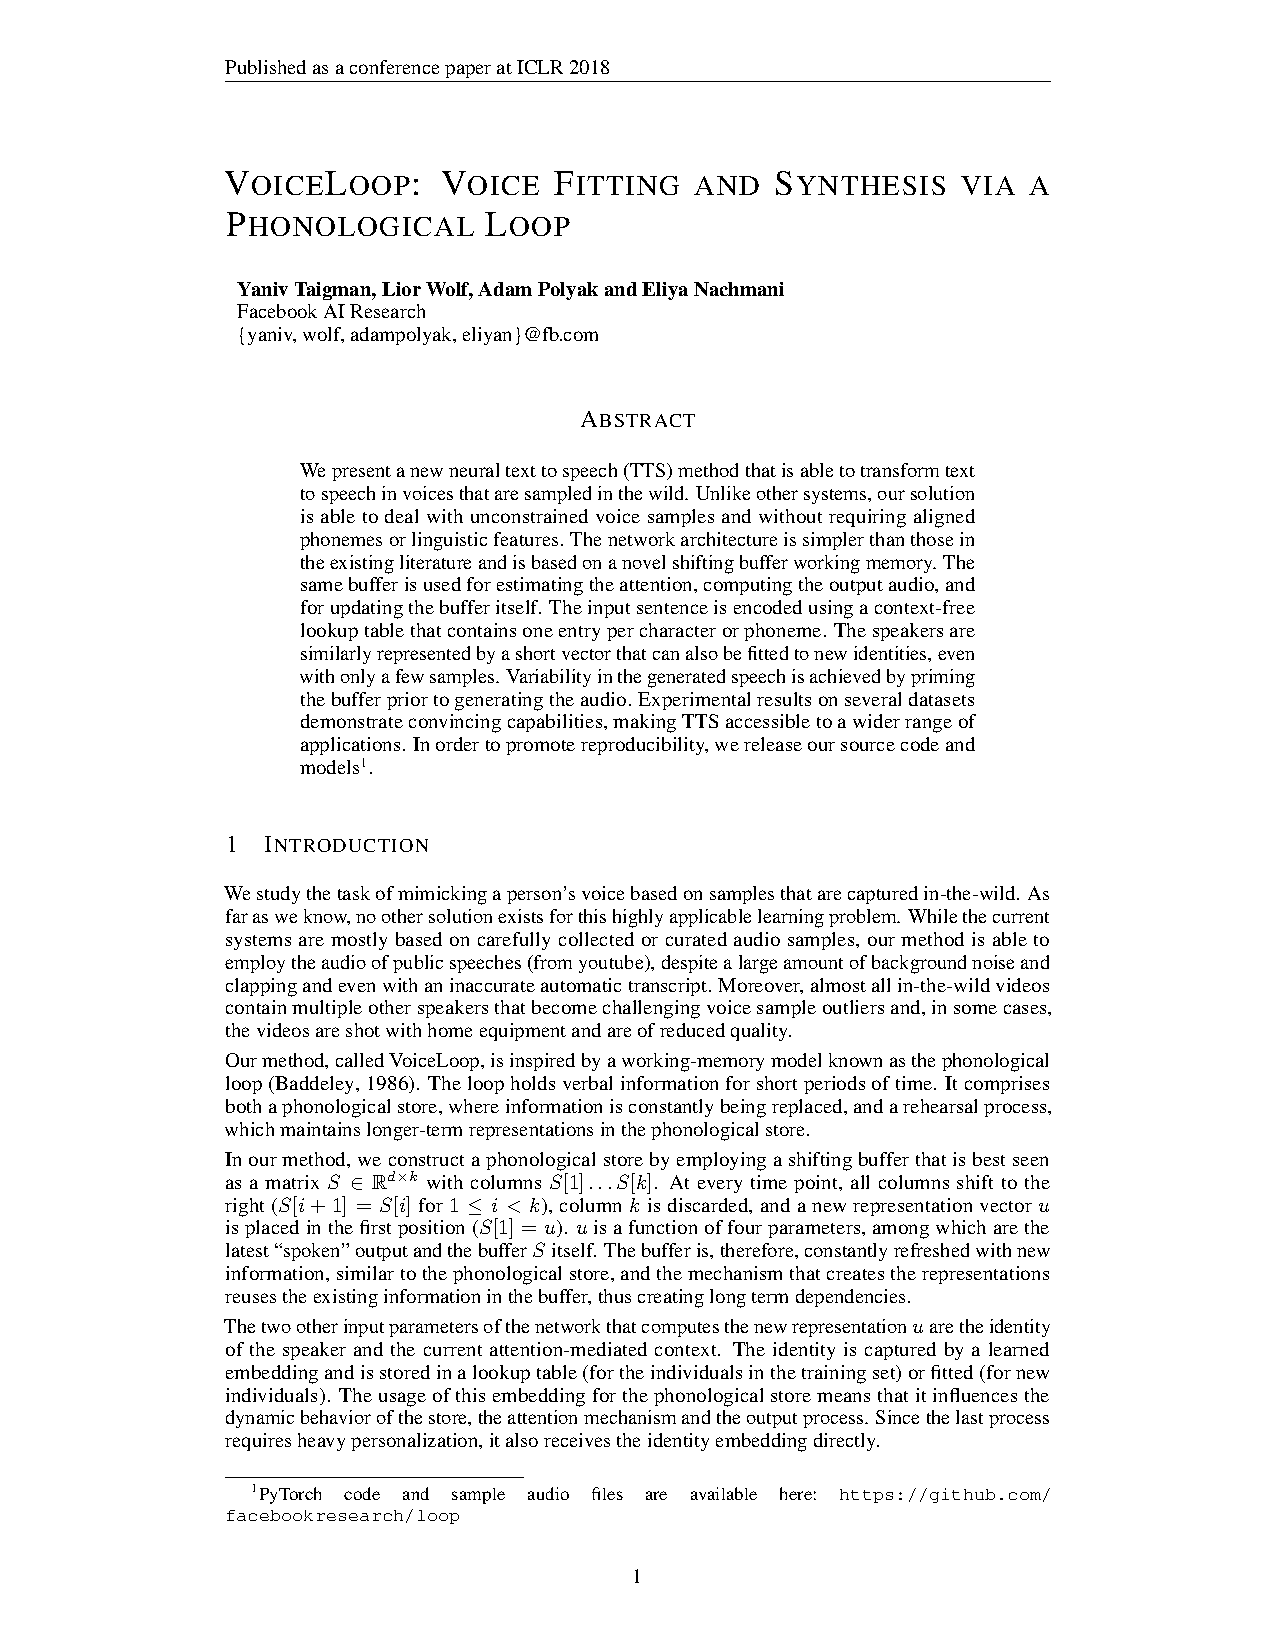
\includegraphics[width=0.95\textwidth]{fig/main.pdf}
\vspace{-14pt}
\caption{Overview of EIGV. It comprises three additional modules on top of the conventional VideoQA backbone: 1) Grounding indicator, 2) Intervener, and 3) Disrupter. First, the grounding indicator learns the estimation of causal scene $\hat{c}$ and environment $\hat{e}$. Next, two interventions are imposed on the causal and non-causal factors to compose the intervened pair $(v^*,q^*)$. Finally, based on the re-grounded result, the disruptor creates contrastive samples, which are further feed into the VideoQA backbone.}
\vspace{-5pt}
\label{fig:main}
\end{figure*}

\wx{
To ground the causal scene $C$ in the video $V$, we take a closer look at the VideoQA SCM (\ie Figure \ref{fig:scm}a), and emphasize the essential differences between $C$ and $E$.
Specifically, given the causal scene $C$ and question $Q$, the answer $A$ is determined, regardless of the variations in the environment scene $E$:}
\begin{gather}\label{equ:eq0}
      A\bot E \mid C,Q,
\end{gather}
where $\bot$ denotes the probabilistic independence. 
%

\vspace{5pt}
\noindent\textbf{Rationalization.} 
During training, the oracle grounding rationale $C$ is out of reach, while only the input $(V, Q)$ pair and training target $A$ are observed. 
Such an absence motivates VideoQA to embrace video grounding in its modeling. 
Specifically, in light of question $Q$, the estimated causal scene $\hat{C}$ is grounded from the massive $V$ to approach the oracle $C$ and then generate prediction $\hat{A}$ via $Q \rightarrow A \leftarrow C$. 
To systematize this relation, the causal-equivariance principle introduces an equivariant transformation $T_\epsilon$ to each of the parent variables (\ie $C$ and $Q$), and expects a proportionate change in the response variable (\ie $A$). On top of SCM, we formally present such notions as:
\begin{gather}
    T_\epsilon(\hat{A})=f_{\hat{A}}(T_\epsilon(\hat{C}),T_\epsilon(Q)). \label{equ:equivariance}
\end{gather}
Meanwhile, environment-invariant principle formulated Equation \eqref{equ:eq0} in the sense that imposing an invariant-transformation $T_\iota$ on the estimated environment $\hat{E}$ should not trigger variation of answer $A$: 
\begin{gather}
      \hat{A}=f_{\hat{A}}(T_\iota(\hat{E}),Q)),\label{equ:invariance}
\end{gather} 
To this end, we parameterize our learning framework, EIGV, as a combination of equivariant and invariant principles, which comprises three additional modules on top of the ERM-guided backbone: grounding indicator, intervener, and disruptor. In a nutshell, we display our EIGV framework in Figure \ref{fig:main}.


\vspace{5pt}
\noindent \textbf{Data representation.}
Following previous efforts \cite{jiang2020reasoning, DBLP:conf/acl/GuoZJ0L20}, we encode video instance $v$ as a sequence of $K$ fixed visual clips, while question instance $q$ is encoded into a similar form with a fixed length of language tokens $L$.
Then, visual and linguistic features are applied with a linear layer and an LSTM \cite{10.1162/neco.1997.9.8.1735}, respectively, to align their dimension. As a result, we acquire the output of linear layer $ \vb{v} \in \mathbb{R}^{k \times d}$ as the final video representation and the last hidden state of LSTM $\vb{q} \in \mathbb{R}^{d}$ as the holistic question representation.

% Following previous efforts [], video instance $v$ is encoded as a sequence of $K$ fixed visual clips $ \vb{v} \in \mathbb{R}^{k \times d_v}$, where $d_v$ is the visual feature dimension. Likewise, the question instance $q$ is encoded into similar form $ \vb{q} \in \mathbb{R}^{L \times d_q}$ but with a fixed length of language tokens L. Furthermore, $\vb{v}$ and $\vb{q}$ are respectively, applied with a linear layer and a LSTM [] to align their dimension, while we acquire the final hidden state of LSTM as a the holistic question representation $\vb{q} \in \mathbb{R}^{d}$.

\subsection{Grounding Indicator}
Scene partition is fundamental to the rationale discovery, whose core is to estimate the value of $C$ and $E$ via a hard split on video $V$. Given an input sample $(v,q)$, the grounding indicator aims to access the causal scene and environment scene via their estimated value $\hat{c}$ and $\hat{e}$ according to question $Q$. 
%
Concretely, we first construct two cross-modal attention modules to indicate the probability of each visual clip of being causal scene ($\vb{p}_{\hat{c}} \in\mathbb{R}^{K}$) 
and environment scene ($\vb{p}_{\hat{e}}\in\mathbb{R}^{K}$):
\begin{align}
    \vb{p}_{\hat{c}} &= \text{Softmax}(\text{FC}_{1}(\vb{v})\cdot\text{FC}_{2}(\vb{q})^\intercal),\\
    \vb{p}_{\hat{t}} &= \text{Softmax}(\text{FC}_{3}(\vb{v})\cdot\text{FC}_{4}(\vb{q})^\intercal),
\end{align}
where $\text{FC}_{1},\text{FC}_{2},\text{FC}_{3},\text{FC}_{4}$ are fully connected layers that align cross-modal representations.
%
However, gathering messages via a soft mask still makes the visual information on different clips overlap. 
As discussed in Section 3.2, guided by ERM, the conventional attention mechanism is unable to block the influence of $\hat{e}$, thus undermining the veracity of $\hat{c}$.
% As revealed by the ERM-guided method, the conventional attention is unable to block the influence of $\hat{t}$ thus undermining the veracity of $\hat{e}$. 
%
As a correction, the grounding indicator makes a discrete selection over the clip-wise attention result to generate a disjoint group of the causal scene. We leverage Gumbel-Softmax \cite{DBLP:conf/iclr/JangGP17} to manage a differentiable selection on attentive probabilities and compute the indicator vector $\vb{I}\in\mathbb{R}^{K\times 2}$ on the two attention scores  over each clip (\ie $\vb{p}_{\hat{c,i}}$, $\vb{p}_{\hat{e,i}}$, $i \in K$).  Formally, $\vb{I}$ is derived as:
\begin{gather}
    \vb{I} = \text{Gumbel-Softmax}([\vb{p}_{\hat{c}};\vb{p}_{\hat{e}}]), 
\end{gather}
where $[;]$ denote concatenation. The first and second column of $\vb{I}$ (\ie $I_{0}$ and $I_{1}$) index the attribution of $\hat{c}$ and $\hat{e}$ over k clips, respectively. 
%
To this end, we estimate $\hat{c}$ and $\hat{e}$ as follows:
\begin{gather}
    \hat{c} = I_{0}\cdot v ,\quad \hat{e} = I_{1}\cdot v, \quad \st v=\hat{c}+\hat{e} .
    % \hat{c} = \{I_{c,k}\cdot v_{k}|I_{c,k}=1\},\quad \hat{t} = \{I_{t,k}\cdot v_{k}|I_{t,k}=1\},
\end{gather}

% where binary masks $I_{0k}$ and $I_{1k}$ indicate the causal-environment attribution of the $k$-th clip.

\subsection{Intervener}
In absence of clip-level supervision, learning grounding indicators requires dedicated exploitation of the equivariance-invariance principle.
%
On this demand, we propose the intervener, which prompts the estimated rationale to the oracle by intervening $\hat{c}$ and $\hat{e}$. 
%
Figure \ref{fig:intervene} describes the functionality of $do(\cdot)$ --- the intervention operator that successively manipulated SCM over $E$ and $C$. Concretely, two intervention operations are configured to realize the equivariant and invariant transformation defined in Equations \eqref{equ:equivariance} and \eqref{equ:invariance}. 
%
% 这块儿写的不清楚。要牢记突出主线:two principle,所有的都是围绕这个实现的,只有我们反复强调这个,才能让reviewer印象深刻,然后才能从idea、implementation层面上都理解我们在干啥,并且觉得我们做的是对的。
% 这里可以分开写:

To fulfill the causal-equivariant principle, we design the E-intervention on the causal scene $\hat{c}$, which applies a linear interpolation between two data points on their causal factors --- $C$, $Q$ and $A$.  
By casting the same mixing ratio $\lambda_0\sim\text{Beta}(\alpha,\alpha)$ on all causal factors, the equivariant intervener learns to capture 
% the mainstay depicted in Figure \ref{fig:scm}c, so as to abridge 
the causal connection of $C, Q \to A$.
In particular, we attain the intervened causal scene $c^*\in \mathbb{R}^{K\times d}$, question $q^*\in \mathbb{R}^{d}$ and answer $a^*\in \mathbb{R}$ as follow:
\begin{gather}
    c^*=\lambda_0 \cdot \hat{c}+(1-\lambda_0) \cdot \hat{c}',\\
    q^*=\lambda_0 \cdot q+(1-\lambda_0) \cdot q',\\
    a^*=\lambda_0 \cdot a+(1-\lambda_0) \cdot a',
\end{gather}
where $\hat{c}'$, $q'$ and $a'$ are causal factors from a second sample.

To achieve the environment-invariant principle, we devise the I-intervention that adopts a similar mixing strategy to the environment scene $\hat{e}$. 
%
Notably, by drawing the mixing ratios $\lambda_1$ from a second distribution that is distinct from the equivariant one (\ie $\lambda_1\sim\text{U}(0,1)$), the invariant intervention learns to rule out the influence of environment scene on the answer, which essentially refines the ERM-guided scheme at our will. 
Formally, we arrive the intervened environment scene $e^*$ by:
\begin{gather}
    e^*=\lambda_1 \cdot \hat{e}+(1-\lambda_1) \cdot \hat{e}',
\end{gather}
where $\hat{e}'$ is the estimated environment scene of a second sample.

In practice, the equvariant and invariant intervention operations are performed in parallel on different parts of $v$, and the intervened video $v^* \in \mathbb{R}^{K\times d}$ is composed of $do(C=c^*)$ and $do(E=e^*)$:
% in a cascade manner:
\begin{gather}
    v^*=c^*+e^*.
\end{gather}

% where $\hat{c}'$ and $\hat{e}'$ are estimate causal and environment scene of dummy  sample ($v',q',a'$).  It's worth noticing that, the mixing ratios $\lambda_0$ and $\lambda_1$ for equivariant and invarinat intervention are drawn from two different distribution, $\lambda_0\sim\text{Beta}(\alpha,\alpha)$ and $\lambda_1\sim\text{U}(0,1)$.
% %
% To complete the reasoning logic, we also apply the equivariant intervention on other causal factors---$Q$ and $A$ to generate intervened question $q^*$ and answer target $a^*$:
% \begin{gather}
%     q^*=\lambda_0 \cdot \hat{q}+(1-\lambda_0) \cdot q',\\
%     a^*=\lambda_1 \cdot \hat{a}+(1-\lambda_1) \cdot a',
% \end{gather}
% Noticably, we cast the same equivariant mixing ratio $\lambda_0$ for $do(Q)$ and $do(A)$ to abridge the the causal connection of $C,Q \to A$. 

% 
\subsection{Disruptor}
% In state-of-the-art self-supervised learning (SSL) pre-training produces semantically good representations by encouraging them to be invariant under meaningful transformations prescribed from human knowledge. 

To fully exploit the privilege of the proposed principles, we employ contrastive learning as an auxiliary objective to establish a good representation that maintains the desired properties of $\hat{c}$ and $\hat{e}$. 
% discribe in  to the counterfactual substitution on $C$($E$). 
Specifically, we first compose a memory bank $\pi$ as a collection of visual clips from other training videos. Then, we apply the grounding indicator a second time on top of the intervened variables, where the re-grounded causal and environment scene are manipulated to set up the contrastive twins as follows:
\begin{itemize}[leftmargin=*]
% 介绍清楚,为啥相对于anchor而言就是positive的
\item In light of the environment-invariance principle, positive video is developed in the sense that changing the environment scene will not provoke disagreement in answer semantics.  Thus, the disruptor synthesizes a positive video $v^+$ by disrupting the $v^*$ on its environment part --- that is, replacing the environment scene with a random stratification sampled from the memory bank.\footnote{Note that the environment substitutes will not involve the question-relevant scenes, to avoid creating additional paths from $E$ to $A$.}  
% 介绍清楚,为啥相对于anchor而言是negaitve的
\item Built upon the causal-equivariance principle, the negative counterpart $v^-$ is created by a similar disruption but on the causal scene of $v^*$, where substitution on the question-critical causal part should raise inconsistency in answer space.
% \footnote{substitution of causal scene substitutes will not involve the question-relevant scenes, to avoid creating additional paths from $E$ to $A$.} 
%
Apart from the visual negatives, the disruptor also creates linguistic alternatives to enhance the distinctiveness of the vision-language alignment. Specifically, it disrupts the combination of the intervened input ($v^*, q^*$) and pairs the video with random sample question $q_r$ to create a second view of negative samples ($v^*, q_r$).
\end{itemize}
To this end, we attain the answer representation of anchor $\vb{a}$ and its contrastive counterparts $\vb{a}^+, \vb{a}^-$ by feeding the paired positive and negative samples to backbone VideoQA model $f_{\hat{A}}$: 
\begin{gather}
    \vb{a}=f_{\hat{A}}(v^*,q^*),\\
    \vb{a}^+=f_{\hat{A}}(v^+,q^*),\\
    \vb{a}^-=f_{\hat{A}}([(v^-,q^*);\,(v^*,q_r)]),
\end{gather}
where $[;]$ denotes concatenation.

Notably, EIGV is designed to be model-agnostic, which aims to promote any VideoQA backbone built on frame-level visual inputs.
%
% Since the architecture modification is beyond our intention, we verify the effectiveness of our design by marrying EIGV to SoTA VideoQA models. 




\subsection{Optimization}
By far, we set up the intervened vision-language instance ($v^*,q^*$) for a pair of input ($v,q$), and further constitute its contrastive counterparts based on the estimated grounding result. 
To steer the learning process away from the conventional ERM pitfall, we establish two learning objectives on top of their output $a, a^+, a^-$:

\begin{itemize}[leftmargin=*]
    \vspace{5pt}
    \item \noindent \textbf{Contrastive loss.} To reflect the invariant property of the environment scene while maintaining the distinctiveness of the causal scene, we borrow the definition of InfoNCE \cite{DBLP:journals/corr/abs-1807-03748}, and construct the contrastive objective as follows:
    \begin{gather}
        \mathcal{L}_{CL}=-log(\frac{\text{exp}{(a^\top a^+)}}{\text{exp}{(a^\top a^+)}\,+\sum_{n}^{N}\text{exp}{(a^\top a_n^-)}}),
    \end{gather}
    where $N$ is the number of negative samples, \lyc{$a_n^-$ denotes negative anwer generated by one of  negative samples.} 
    
    \vspace{5pt}
    \item \noindent \textbf{ERM loss.} 
    Estimating the rationale requires a robust causal connection from $V,Q$ to $A$. Thus, we imposed an entropy-based risk function \lyc{$\text{XE}(\cdot)$} on $(v^*,q^*)$ to approach the intervened answer $a^*$:
    \begin{gather}
        \mathcal{L}_{ERM}=\text{XE}(f_{\hat{A}}(v^*,q^*), a^*),
    \end{gather}
\end{itemize}

As a result, the overall training objective of EIGV is the aggregation of the forgoing risks:
\begin{gather}
   \mathcal{L}_{\text{EIGV}} = \mathbb{E}_{(v,q,a)\in\mathcal{O}}\mathcal{L}_{ERM} + \beta\mathcal{L}_{CL},
\end{gather}
where $\mathcal{O}$ is the set of training instances $(v,q)$ alongside their ground-truth answer $a$; $\beta$ is the hyper-parameter that balances the strength of contrastive learning. The joint optimization disentangles the mischief of environment scene, thus fulfilling the desired interpretation by locating the causal pattern. During inference, EIGV generates the predication $\hat{a}$ without the intervener and disruptor involved, and gives the interpretation $\hat{c}$ as the partition result of the grounding indicator.

% Specifically, by minizing the  the similarity between en-
% coded representations of the same video at two
% different speeds as well as minimize the sim-
% ilarity between different videos played at dif-
% ferent speeds, leveraging the fact that changing
% video speed does not change an action on both
% domains.


% an oracle interpretation $C$ should reflect the semantic variance of different $Q$ and trigger the corresponding change in $A$,

% video input tend to contain multiple visual scene, but only the question-relevant part contributes to the prediction while the rest is inconsequential to the reasoning logic.


\begin{figure}[t]
\centering
\includegraphics[scale=0.43]{fig/intervene.pdf}
\caption{We illustrate the invariant and equivariant interventions in the second and third rows, respectively. The effects on $Q$ and $A$ are omitted for illustration purposes.}
\vspace{-5pt}
\label{fig:intervene}
\end{figure}
\section{Experiment}
\label{sec:experiment}

In this section, we show the experimental results to answer the following research questions.
\begin{itemize}[leftmargin=*]
\item \textbf{RQ1} How effective is EIGV in discovering the causal pattern and improving the model generalization across different settings?
\item \textbf{RQ2} How does the sub-module and feature setting contribute to the performance?
\item \textbf{RQ3} What pattern does EIGV capture in rationale discovery?
\end{itemize}

\subsection{Settings}

\vspace{5pt}
\noindent \textbf{Datasets.} We conduct experiments on three benchmark datasets that challenge the model's reasoning capacity from different aspects: 
\textbf{MSVD-QA}  \cite{DBLP:conf/mm/XuZX0Z0Z17} and \textbf{MSRVTT-QA} \cite{DBLP:conf/mm/XuZX0Z0Z17} mainly emphasize the recognition ability by asking the descriptive questions, where 50K and 243K question-answer pairs are automatically generated from the human-labeled video captions, respectively.
\textbf{NExT-QA} \cite{DBLP:conf/cvpr/XiaoSYC21} pinpoints the causal and temporal relations among objects in the video. It contains 47.7K questions with answers in the form of multi-choice, which are manually annotated from 5.4K videos.

\vspace{5pt}
\noindent\textbf{Baseline.} We validate the effectiveness of EIGV across backbone VideoQA models of three kinds: 
1) \textbf{Memory-based} methods that foster a storage of input sequence via auxiliary memory design, such as AMU \cite{DBLP:conf/mm/XuZX0Z0Z17}, HME \cite{fan2019heterogeneous} and Co-Mem \cite{gao2018motionappearance}.
2) \textbf{Graph-based} methods that leverage the expressiveness of graph network to model the interaction between visual and language elements, which involves methods like L-GCN \cite{huang2020locationaware}, B2A  \cite{park2021bridge} and HGA \cite{jiang2020reasoning}. 
3) \textbf{Hierarchy-based} methods include HCRN \cite{le2021hierarchical}, PGAT \cite{DBLP:conf/mm/PengYBW21}, HOSTR \cite{dang2021hierarchical}, MSPAN \cite{DBLP:conf/acl/GuoZJ0L20} and HQGA \cite{xiao2021video}. In common, they exploit the multi-granularity nature of visual elements and realize the hierarchical reasoning via bottom-up architecture. 
In Specific, we test the generalization of EIGV by marrying our learning principles to three backbones of different categories: memory-based Co-Mem \cite{gao2018motionappearance}, graph-based HGA \cite{jiang2020reasoning} and hierarchy-based MSPAN \cite{DBLP:conf/acl/GuoZJ0L20}. 

\vspace{5pt}
\noindent \textbf{Implementation Detail.} 
For input representation, we encode the video instance as a sequence of $K$=16 clips, where each clip is represented as a combination of appearance and motion features extracted from the pre-trained ResNet-152 and 3D ResNeXt-101. For the linguistic feature, we follow \cite{DBLP:conf/cvpr/XiaoSYC21} and obtain the contextualized word representation using the fine-tuned BERT model. In the hyper-parameters setting, we set $d=512$ for cross-modal alignment, then train the model for 80 epochs with an initial learning rate of 5e-5.  During optimization, EIGV is trained with Adam optimizer and we decay the learning rate when validation stops improving for 5 epochs. The balance ratio $\beta$ is set to 0.75.
%for open-set QA and 0.025 for multi-choice QA. 

\subsection{Main Result (RQ1)}
\def\year{2019}\relax
%File: formatting-instruction.tex
\documentclass[letterpaper]{article} %DO NOT CHANGE THIS
% \usepackage{aaai19}  %Required
\usepackage{arXiv}  % for arXiv  <<<<<<<<<<<<<<<<<<<<<<<<<<<<<<<<<<<<<<<<<<<<<<<<<<<
\usepackage{times}  %Required
\usepackage{helvet}  %Required
\usepackage{courier}  %Required
\usepackage{url}  %Required
\usepackage{graphicx}  %Required
\frenchspacing  %Required
\setlength{\pdfpagewidth}{8.5in}  %Required
\setlength{\pdfpageheight}{11in}  %Required

% DY added
% \usepackage[final]{hyperref}
\usepackage{multirow}
\usepackage{amsmath}
\usepackage{subfig}
% \usepackage{subcaption}

% \usepackage{caption}
\usepackage{multirow}
\usepackage{bbm}

\usepackage{xcolor}
\usepackage{colortbl}
\usepackage{array}
\usepackage{pifont}
\usepackage{booktabs}


%PDF Info Is Required:
  \pdfinfo{
/Title (Utilizing Class Information for Deep Network Representation Shaping)
/Author (Daeyoung Choi, Wonjong Rhee)}
\setcounter{secnumdepth}{0}  
% \setcounter{secnumdepth}{2} % for arXiv <<<<<<<<<<<<<<<<<<<<<<<<<<<<<<<<<<<<<<<<<<<<<<<<<<<

\begin{document}
% The file aaai.sty is the style file for AAAI Press 
% proceedings, working notes, and technical reports.
%
\title{Utilizing Class Information for Deep Network Representation Shaping}

\author{Daeyoung Choi\thanks{Authors contributed equally.} and Wonjong Rhee\footnotemark[1] \\
Department of Transdisciplinary Studies\\
Seoul National University\\
Seoul, 08826, South Korea \\
\texttt{\{choid, wrhee\}@snu.ac.kr} 
}
\maketitle
\begin{abstract}
Statistical characteristics of deep network representations, such as sparsity and correlation, are known to be relevant to the performance and interpretability of deep learning. When a statistical characteristic is desired, often an adequate regularizer can be designed and applied during the training phase. Typically, such a regularizer aims to manipulate a statistical characteristic over all classes together. For classification tasks, however, it might be advantageous to enforce the desired characteristic per class such that different classes can be better distinguished. Motivated by the idea, we design two class-wise regularizers that explicitly utilize class information: class-wise Covariance Regularizer (cw-CR) and class-wise Variance Regularizer (cw-VR). cw-CR targets to reduce the covariance of representations calculated from the same class samples for encouraging feature independence. cw-VR is similar, but variance instead of covariance is targeted to improve feature compactness. For the sake of completeness, their counterparts without using class information, Covariance Regularizer (CR) and Variance Regularizer (VR), are considered together. The four regularizers are conceptually simple and computationally very efficient, and the visualization shows that the regularizers indeed perform distinct representation shaping. In terms of classification performance, significant improvements over the baseline and L1/L2 weight regularization methods were found for 21 out of 22 tasks over popular benchmark datasets. In particular, cw-VR achieved the best performance for 13 tasks including ResNet-32/110. 
\end{abstract}


%=============================================
% #Introduction
%=============================================

\section{Introduction}
%

\begin{figure}[t]
% \vskip 0.1in
\centering
\centerline{\includegraphics[width=8.25cm]{mnist_none_hist_scatter.pdf}}
\caption{
% \small{
A single unit's activation histogram (upper three plots) and two randomly chosen units' activation scatter plots (lower three plots) for MNIST. For a 6-layer Multilayer Perceptron (MLP), the fifth layer's representation vectors calculated using 10,000 test samples were used to generate the plots. For the baseline model, a substantial overlap among different classes can be observed at the time of initialization as shown in (a). Even after 50 epochs of training, still, a substantial overlap can be observed as shown in (b). When class information is used to regularize the representation shapes, the overlap is significantly reduced as shown in (c). Note that a slight correlation between each pair of classes can be observed in the scatter plot of (b), but not in that of (c) due to the use of cw-CR. The figures are best viewed in color.
% }
}
\label{fig:mnist_none_hist_scatter}
% \vskip -0.3in
\end{figure}

For deep learning, a variety of regularization techniques have been developed by focusing on the \textit{weight parameters}. A classic example is the use of L2 \cite{hoerl1970ridge} and L1 \cite{tibshirani1996regression} weight regularizers. They have been popular because they are easy to use, computationally light, and often result in performance enhancements. Another example is the parameter sharing technique that enforces the same weight values as in the Convolutional Neural Networks (CNNs).  
Regularization techniques that focus on the \textit{representation} (the activations of the units in a deep network), however, have been less popular even though the performance of deep learning is known to depend on the learned representation heavily. 

For representation shaping (regularization), some of the promising methods for performance and interpretability include \cite{glorot2011deep,cogswell2015reducing,liao2016learning}.
\cite{glorot2011deep} considers increasing representational sparsity, \cite{cogswell2015reducing} focuses on reducing covariance among hidden units, and \cite{liao2016learning} forces parsimonious representations using k-means style clustering. While all of them are effective representation regularizers, none of them explicitly use class information for the regularization. A few recent works \cite{wen2016discriminative,belharbi2017neural,yang2018robust} do utilize class information, and their approaches are based on \textit{hidden layer activation vectors}. The method of \cite{belharbi2017neural} is computationally expensive because pair-wise dissimilarities need to be calculated among the same class samples in each mini-batch. 

In this work, two computationally light representation regularizers, cw-CR (class-wise Covariance Regularizer) and cw-VR (class-wise Variance Regularizer), that utilize class information are introduced and studied. We came up with the design ideas by observing typical histograms and scatter plots of deep networks as shown in Figure \ref{fig:mnist_none_hist_scatter}. In Figure \ref{fig:mnist_none_hist_scatter} (b), different classes substantially overlap even after the training is complete. If we directly use class information in regularization, as opposed to using it only for cross-entropy cost calculation, we can specifically reduce overlaps or pursue a desired representation characteristic. An example of cw-CR reducing class-wise covariance is shown in Figure \ref{fig:mnist_none_hist_scatter} (c), and later we will show that cw-VR can notably reduce class-wise variance resulting in minimal overlaps. The two class-wise regularizers are very simple and computationally efficient, and therefore can be easily used as L1 or L2 weight regularizers that are very popular. 

% our contributions
\subsection{Our Contributions}
The contributions of this work can be summarized as follows.

\subsubsection{Introduction of three new representation regularizers} 
We introduce two representation regularizers that utilize class information. cw-CR and cw-VR reduce per-class covariance and variance, respectively. In this work, their penalty loss functions are defined, and their gradients are analyzed and interpreted. Also, we investigate VR that is cw-VR's all-class counterpart. Intuitively, reducing the variance of each unit's activations does not make sense unless it is applied per class, but we have tried VR for the sake of completeness and found that VR is useful for performance enhancement. cw-CR's all-class counterpart, CR, is analyzed as well, but CR turns out to be the same as DeCov that was already studied in-depth in \cite{cogswell2015reducing}. 

\subsubsection{Performance improvement with the new representation regularizers}
Rather than trying to find a single case of beating the state-of-the-art record, we performed an extensive set of experiments on the most popular datasets (MNIST, CIFAR-10, CIFAR-100) and architectures (MLP, CNN). Additionally, ResNet \cite{he2016deep} was tested as an example of a sophisticated network, and an image reconstruction task using autoencoder was tested as an example of a different type of task. We have tested a variety of scenarios with different optimizers, number of classes, network size, and data size. The results show that our representation regularizers outperform the baseline (no regularizer) and L1/L2 weight regularizers for almost all the scenarios that we have tested. More importantly, class-wise regularizers (cw-CR, cw-VR) usually outperformed their all-class counterparts (CR, VR). Typically cw-VR was the best performing regularizer and achieved the best performance for the autoencoder task, too.

\subsubsection{Effects of representation regularization}
Through visualizations and quantitative analyses, we show that the new representation regularizers indeed shape representations in the ways that we have intended. The quantitative analysis of representation characteristics, however, indicates that each regularizer affects multiple representation characteristics together and therefore the regularizers cannot be used to control a single representation characteristic without at least mildly affecting some other representation characteristics. 


%=============================================
% #Related Works
%=============================================

\section{Related Works}

\subsection{Regularization for Deep Learning}
%
The classic regularizers apply L2 \cite{hoerl1970ridge} and L1 \cite{tibshirani1996regression} 
penalties to the \textit{weights} of models, and they are widely used for Deep Neural Networks (DNNs) as well. 
%
\cite{wen2016learning} extended L1 regularizers by using group lasso to regularize 
the structures of DNN (i.e., filters, channels, filter shapes, and layer depth).
%
\cite{srivastava2014dropout} devised dropout that randomly applies activation masking 
over the units.
%
While dropout is applied in a multiplicative manner, \cite{glorot2011deep} used L1 penalty 
regularization on the activations to encourage sparse representations.
%
XCov proposed by \cite{cheung2014discovering} minimizes the covariance between 
autoencoding units and label encoding units of the same layer such that 
representations can be disentangled.  
%
Batch normalization (BN) proposed by \cite{ioffe2015batch} exploits mini-batch statistics 
to normalize activations. It was developed to accelerate training speed by preventing 
internal covariate shift, but it was also found to be a useful regularizer.
%
In line with batch normalization, weight normalization, developed by \cite{salimans2016weight}, 
uses mini-batch statistics to normalize weight vectors. 
%
Layer normalization proposed by \cite{ba2016layer} is a RNN version of batch normalization,
where they compute the mean and variance used for normalization from all of the summed
inputs to the units in a layer on a single training case.
%
There are many other publications on regularization techniques for deep learning,
but we still do not fully understand how they really affect the performance.  
Recent work by \cite{zhang2016understanding}
shows that the traditional concept of controlling generalization error by regularizing the effective capacity does not apply to the modern DNNs. 


\subsection{Penalty Regularization on Representations}
Some of the existing regularization methods explicitly shape representations by adopting a penalty regularization term.
%
DeCov \cite{cogswell2015reducing} is a penalty regularizer that minimizes the off-diagonals of a layer's representation covariance matrix. DeCov reduces co-adaptation of a layer's units by encouraging the units to be decorrelated. In this work, 
it is called as CR (Covariance Regularizer) for consistent naming.
%
A recent work \cite{liao2016learning} used a clustering based regularization that encourages parsimonious representations. In their work, similar representations in sample, spatial, and channel dimensions are clustered and used for regularization such that similar representations are encouraged to become even more similar. While their work can be applied to unsupervised as well as supervised tasks, our work utilizes a much simpler and computationally efficient method of directly using class labels during training to avoid k-means like clustering. 

\subsection{Class-wise Learning}
True class information has been rarely used directly for regularization methods.
Traditionally, the class information has been used only for evaluating the correctness of
predictions and the relevant cost function terms. Some of the recent works, however, 
have adopted the class-wise concept in more sophisticated ways. In those works, 
class information is used as a switch or for emphasizing the discriminative aspects over different classes. 
%
As an example, \cite{li2008kernel} proposed a kernel learning method using class information to model the manifold structure. They modify locality preserving projection to be class dependent. \cite{jiang2011learning} 
added label consistent regularizers for learning a discriminative dictionary. 
%
\cite{wen2016discriminative} developed a regularizer called center loss that reduces the activation vector distance between representations and their corresponding class centers for face recognition tasks.
%
\cite{yang2018robust} designed a loss function named prototype loss that improves representation's intra-class compactness for enhancing the robustness of CNN.
%
Another recent work by \cite{belharbi2017neural} directly uses class labels to encourage similar representations per class as in our work, but it is computationally heavy as explained earlier.  
Besides the pair-wise computation, two optimizers are used for handling the supervised loss term and the hint term separately. 
%
Class information is used for autoencoder tasks as well. \cite{shi2016learning} implicitly reduced the intra-class variation of reconstructed samples by minimizing pair-wise distances among same class samples.
%
Like the strategies listed above, our cw-VR and cw-CR use class-wise information to control the statistical characteristics of representations. However, our methods are simple because only one optimizer is used, and computationally efficient because pair-wise computation is not required.


%=============================================
% #Class-wise Representation Regularizers
%=============================================

\section{Class-wise Representation Regularizers: cw-CR and cw-VR}

In this section, we first present basic statistics of representations. Then, three representation regularizers, cw-CR, cw-VR, and VR are introduced with their penalty loss functions and gradients. Interpretations of the loss functions and gradients are provided as well. 

\subsection{Basic Statistics of Representations}
\label{subsection:stats}
For the layer $l$, the output activation vector of the layer is defined as 
$\mathbf{z}_l = \max(\mathbf{W}^\top_l \mathbf{z}_{l-1} + \mathbf{b}_l, 0)$ using Rectified Linear Unit (ReLU)
activation function. Because we will be focusing on the layer $l$ for most of the explanations, 
we drop the layer index. 
Then, $z_i$ is the $i^{th}$ element of $\mathbf{z}$ (i.e. activation of $i^{th}$ unit). 
%  ,and $w_{ki}$ is the $(k,i)$ element of $\mathbf{W}$. 

To use statistical properties of representations, we define mean of unit $i$, $\mu_i$, and covariance 
between unit $i$ and unit $j$, $\textit{c}_{i,j}$, using the $N$ samples in each mini-batch. 
\begin{align}
    \mu_i &= \frac{1}{N} \sum_n z_{i,n}  \label{eq:mean}  \\
    \textit{c}_{i,j} &= \frac{1}{N} \sum_n (z_{i,n} - \mu_i)(z_{j,n} - \mu_j) \label{eq:covariance}
\end{align}
Here, $z_{i,n}$ is the activation of unit $i$ for $n^{th}$ sample in the mini-batch.  
From equation (\ref{eq:covariance}), variance of $i$ unit can be written as the following. 
\begin{align}
    \textit{v}_{i} &= \textit{c}_{i,i} \label{eq:variance}
\end{align}
When class-wise statistics need to be considered, we choose a single label $k$ from $K$ labels
and evaluate mean, covariance, and variance using only the data samples with true label $k$
in the mini-batch. 
\begin{align}
    \mu_i^k &= \frac{1}{|S_k|} \sum_{n \in S_k} z_{i,n} \label{eq:mean_cw} \\
    \textit{c}_{i,j}^k &= \frac{1}{|S_k|} \sum_{n \in S_k} (z_{i,n} - \mu_i^k)(z_{j,n} - \mu_j^k) \label{eq:covariance_cw}  \\  
    \textit{v}_{i}^k &= \textit{c}_{i,i}^k   \label{eq:variance_cw}
\end{align}
Here, $S_k$ is the set containing indexes of the samples whose true label is $k$, 
and $|S_k|$ is the cardinality of the set $S_k$.

\begin{table*}[t]
\caption{Penalty loss functions and gradients of the representation regularizers. All the penalty loss functions are normalized with the number of units ($I$) and the number of classes ($K$) such that the value of $\lambda$ can have a consistent meaning. CR and cw-CR are standardized using the number of distinct covariance combinations.}
% \vskip 0.15in
\centering
% \begin{small}
% \setlength{\tabcolsep}{8pt} % Default value: 6pt
% \renewcommand{\arraystretch}{2} % Default value: 1
\begin{tabular}{rlrl}
		\hline
		\multicolumn{2}{c}{Penalty loss function}  & \multicolumn{2}{c}{Gradient}  \\ \hline
		$\displaystyle{\Omega}_{CR}$ & $\displaystyle=\frac{2}{I(I-1)}\sum_{i\neq j} (c_{i,j})^{2} $    & $\displaystyle\frac{\partial{{\Omega}_{CR}}}{\partial{z_{i,n}}}$ & $\displaystyle=\frac{4}{NI(I-1)}\sum_{j\neq{i}}^{}{c_{i,j}(z_{j,n}-\mu_{j}})$  \\ 
		
		$\displaystyle{\Omega}_{cw{\text -}CR}$ & $\displaystyle=\frac{2}{KI(I-1)}\sum_k \sum_{i\neq j} (c_{i,j}^{k})^{2} $   & $\displaystyle\frac{\partial{{\Omega}_{cw{\text-}CR}}}{\partial{z_{i,n}}}$ & $\displaystyle=\frac{4}{KI(I-1)|S_k|}\sum_{j\neq{i}}^{}{c_{i,j}^{k}(z_{j,n}-\mu_{j}^{k}}),  n \in S_k$  \\ 
		
		$\displaystyle{\Omega}_{VR}$ & $\displaystyle=\frac{1}{I}\sum_i v_{i}$                                               & $\displaystyle\frac{\partial{{\Omega}_{VR}}}{\partial{z_{i,n}}}$ & $\displaystyle=\frac{2}{NI}(z_{i,n}-\mu_{i})$  \\
		
		$\displaystyle{\Omega}_{cw{\text -}VR}$ & $\displaystyle=\frac{1}{K I}\sum_k \sum_i v_{i}^k $                        & $\displaystyle\frac{\partial{{\Omega}_{cw{\text -}VR}}}{\partial{{z}_{i,n}}}$ & $\displaystyle =\frac{2}{KI|S_k|}({z}_{i,n}-{\mu}_{i}^{k}), n \in S_k$  \\ \hline
	\end{tabular}
% \end{small}
\label{table:loss_function}
% \vskip -0.2in
\end{table*}

\subsection{cw-CR}
cw-CR uses off-diagonal terms of the mini-batch covariance matrix of activations per class as the penalty term: ${\Omega}_{cw{\text -}CR}=\sum_k \sum_{i\neq j} (c_{i,j}^{k})^{2}$. This term is added to the original cost function $J$, and the total cost function $\widetilde{J}$ can be denoted as  
\begin{align}
    \widetilde{J}=J+\lambda{\Omega}_{cw{\text -}CR}(\mathbf{z}),
\end{align}
where $\lambda$ is the penalty loss weight ($\lambda \in [0, \infty)$). The penalty loss weight balances between the original cost function $J$ and the penalty loss term $\Omega$. When $\lambda$ is equal to zero, $\widetilde{J}$ is the same as $J$, and cw-CR does not influence the network. When $\lambda$ is a positive number, the network is regularized by cw-CR, and the performance is affected. In practice, we have observed that deep networks with too large $\lambda$ cannot be trained at all.

\subsection{cw-VR}
A very intuitive way of enforcing distinguished representations per class is to maximize the inter-class distances in the representation space. 
%However, such a distance maximizer turns out to be difficult to implement as a penalty loss function because the cost function needs to be maximized and not minimized. 
%We implemented the idea and applied the regularizer, but the optimization became unstable (failed to converge). 
%Inter-class distance needs to be maximized. To include the penalty term to the cost function (that needs to be minimized), we tried inversion and multiplication by -1. Both caused the optimization to diverge. 
Because inter-class needs to be maximized, the corresponding penalty term can be inverted or multiplied by -1 before it is minimized with the original cost function. 
We tried such approaches, but the optimization became unstable (failed to converge).
%
An alternative way is to reduce intra-class (same-class) variance. By applying this idea, the penalty loss term of cw-VR can be formulated as ${\Omega}_{cw{\text -}VR}=\sum_k \sum_i v_{i}^k$. 

With the design of cw-VR, we naturally invented VR that is the all-class counterpart of cw-VR. VR minimizes the activation variance of each unit, and it is mostly the same as cw-VR except for not using the class information. We expected VR to hurt the performance of deep networks because it encourages all classes to have similar representation in each unit. VR, however, turned out to be effective and useful for performance enhancement. We provide a possible explanation in the Experiments section. 

\subsection{Penalty Loss Functions and Gradients}

The penalty loss functions of cw-CR and cw-VR are similar to CR and VR, respectively, except that the values are calculated for each class using the mini-batch samples with the same class label. Also, gradients of CR and cw-CR are related to those of VR and cw-VR as shown in Table \ref{table:loss_function}. We investigate more details of the equations in the following.

\subsubsection{Interpretation of the gradients}
Among the gradient equations shown in Table \ref{table:loss_function}, the easiest to understand is VR's gradient. It contains the term ${z}_{i,n}-{\mu}_{i}$, indicating that the representation ${z}_{i,n}$ of each sample $n$ is encouraged to become closer to the mean activation ${\mu}_{i}$. In this way, each unit's variance can be reduced. For cw-VR, the equation contains ${z}_{i,n}-{\mu}_{i}^{k}$ instead of ${z}_{i,n}-{\mu}_{i}$. Therefore the representation ${z}_{i,n}$ of a class $k$ sample is encouraged to become closer to the \textit{class} mean activation ${\mu}_{i}^{k}$. Clearly, the variance reduction is applied per class by cw-VR. 

For CR, the equation is less straightforward. As explained in \cite{cogswell2015reducing}, a possible interpretation is that the covariance term $c_{i,j}$ is encouraged to be reduced where $z_{j,n}-\mu_j$ acts as the weight. But, another possible interpretation is that $z_{j,n}$ is encouraged to become closer to $\mu_j$ just as in the case of VR, where $c_{i,j}$ acts as the weight. Note that VR's mechanism is straightforward where each unit's variance is directly addressed in the gradient equation of activation $i$, but CR's mechanism is slightly complicated where all variances over all activations of $j$ ($j=1,...,I$, where $j \neq i$) are collectively addressed through the summation terms over all $j$ ($j=1,...,I$, where $j \neq i$). Thus, one can interpret CR as a hybrid regularizer that wants either or both of covariance and variance to be reduced. This can be the reason why the visualizations of CR and VR are similar as will be shown in Figure \ref{fig:representation} later. 

For cw-CR, it can be interpreted similarly. As in the relationship between VR and cw-VR, cw-CR is the class-wise counterpart of CR and it can be confirmed in the gradient equation: cw-CR has $c_{i,j}^k({z}_{j,n}-{\mu}_{j}^{k})$ instead of $c_{i,j}({z}_{j,n}-{\mu}_{j})$. As in our explanation of CR, cw-CR can also be interpreted as trying to reduce either or both of covariance and variance. The visualizations of cw-CR and cw-VR turn out to be similar as well. 

The interpretations can be summarized as follows. VR and cw-VR aim to reduce activation variance whereas CR and cw-CR additionally aim to reduce covariance. CR and VR do not distinguish among different classes, but cw-CR and cw-VR explicitly perform representation shaping per class.

\subsubsection{Activation squashing effect}
There is another important effect that is not necessarily obvious from the gradient formulations.
For L1W (L1 weight regularization) and L2W (L2 weight regularization), the gradients contain the weight terms, and therefore the weights are explicitly encouraged to become smaller. Similarly, our representation regularizers include the activation terms $z_{i,n}$ and therefore the activations are explicitly encouraged to become smaller (when activations become close to zero, the mean terms become close to zero as well). Thus, a simple way to reduce the penalty loss is to scale the activations to small values instead of satisfying the balance between the terms in the gradient equations. 
This means that there is a chance for the learning algorithm to squash activations just so that the representation regularization term can be ignored. As we will see later in the next section, indeed activation squashing happens when our regularizers are applied. Nonetheless, we will also show that the desired statistical properties are sufficiently manifested anyway. One might be able to prevent activation squashing with another regularization technique, but such an experiment was not in the scope of this work. 


%=============================================
% Experiments
%=============================================

\section{Experiments}
\label{sec:experiments}
In this section, we investigate performance improvements of the four representation regularizers, where baseline, L1W, L2W, CR, cw-CR, VR, and cw-VR are evaluated for image classification and reconstruction tasks. When a regularizer (including L1W and L2W) was used for an evaluation scenario, the penalty loss weight $\lambda$ was determined as one of \{0.001, 0.01, 0.1, 1, 10, 100\} using 10,000 validation samples. Once the $\lambda$ was determined, performance evaluation was repeated five times. Code is made available at
\url{https://github.com/snu-adsl/class_wise_regularizer}.

\subsection{Image Classification Task}
\begin{table}[t]
\centering
\caption{Error performance (\%) for CIFAR-10 CNN model.}
\label{table:cifar-10}
% \setlength{\tabcolsep}{10pt} % Default value: 6pt
\begin{tabular}{ccc}
\hline
\multirow{2}{*}{Regularizer} & \multicolumn{2}{c}{Optimizer}                      \\ \cline{2-3} 
                             & Adam                                    & Momentum \\ \hline
Baseline                     & $26.64 \pm 0.16$                        & $25.78 \pm 0.37$ \\ \hline
L1W                          & $26.46 \pm 0.39$                        & $25.73 \pm 0.40$ \\
L2W                          & $25.71 \pm 0.98$                        & $26.35 \pm 0.54$ \\ \hline
CR                           & $24.96 \pm 0.63$                        & $26.72 \pm 0.61$ \\ 
cw-CR                        & $22.99 \pm 0.58$                        & $25.93 \pm 0.59$ \\
VR                           & \pmb{$21.44 \pm 0.88$}                  & $25.01 \pm 0.41$ \\
cw-VR                        & $21.58 \pm 0.21$                        & \pmb{$24.42 \pm 0.31$} \\ \hline
% L1R (will be removed)        & $20.62 \pm 0.50$                        & $26.49 \pm 0.96$ \\ \hline
\end{tabular}
% \vskip -0.1in
\end{table}
% \bigskip
\begin{table}[t]
\centering
\caption{Error performance (\%) for CIFAR-100 CNN model.}
\label{table:cifar-100}
\resizebox{\columnwidth}{!}{%
% \setlength{\tabcolsep}{4pt} % Default value: 6pt
\begin{tabular}{cccc}
\hline
\multirow{2}{*}{Regularizer} & \multicolumn{3}{c}{Number of Classes}                                                                                       \\ \cline{2-4}
                                                                   & 16                                      & 64            & 100                         \\ \hline
Baseline    & $45.75 \pm 0.73$                  & $58.02 \pm 0.40$       & $61.26 \pm 0.52$                 \\ \hline
L1W         & $45.08 \pm 1.53$                  & $58.08 \pm 1.18$       & $60.97 \pm 0.64$                 \\
L2W         & $45.28 \pm 1.59$                  & $57.47 \pm 0.66$       & $60.23 \pm 0.31$                 \\ \hline
CR          & $44.55 \pm 1.10$                  & $56.76 \pm 0.86$       & $59.88 \pm 0.50$                 \\ 
cw-CR       & $43.50 \pm 1.21$                  & $54.24 \pm 0.64$       & $57.03 \pm 0.73$                 \\
VR          & $42.33 \pm 1.03$                  & $54.32 \pm 0.40$       & $57.68 \pm 0.94$                  \\
cw-VR       & \pmb{$41.38 \pm 0.53$}            & \pmb{$54.23 \pm 1.06$} & \pmb{$56.75 \pm 0.64$}             \\ \hline
% L1R (will be removed)   & $42.51 \pm 1.43$      & $53.65 \pm 1.00$       & $56.03 \pm 0.81$                  \\ \hline
\end{tabular}
}
% \vskip -0.15in
\end{table}

Three popular datasets (MNIST, CIFAR-10, and CIFAR-100) were used as benchmarks. An MLP model was used for MNIST, and a CNN model was used for CIFAR-10/100. The details of the architecture hyperparameters can be found in Section A of the supplementary materials. All the regularizers were applied to the fifth layer of the 6-layer MLP model and the fully connected layer of the CNN model, and the reason will be explained in the Layer Dependency section. For L1W and L2W, we applied regularization to all the layers as well for comparison, but the performance results were comparable to when applied to the fifth layer. Mini-batch size was increased to 500 for CIFAR-100 such that class-wise operations can be appropriately performed but was kept at the default value of 100 for MNIST and CIFAR-10. We have tested a total of 20 scenarios where the choice of an optimizer, number of classes, network size, or data size was varied.

The results for two CIFAR-10 CNN scenarios are shown in Table \ref{table:cifar-10} and three CIFAR-100 CNN scenarios are shown in Table \ref{table:cifar-100}. The rest of the scenarios including full cases of MNIST MLP can be found in Section B of the supplementary materials. In the Table \ref{table:cifar-10} and Table \ref{table:cifar-100}, it can be seen that cw-VR achieves the best performance in 4 out of 5 cases and class-wise regularizers perform better than their all-class counterparts except for one case. For the scenarios shown in Table \ref{table:cifar-100}, we initially guessed that the performance of class-wise regularizers would be sensitive to the number of classes, but cw-VR performed well for all three cases. As for the 20 scenarios that were tested, the best performing one was cw-VR for 11 cases, VR for 5 cases, cw-CR for 2 cases, and CR for 1 case. L1W and L2W were never the best performing one, and the baseline (no regularization) performed the best for only one case. 

As mentioned earlier, in general, VR did not hurt performance compared to the baseline. There are two possible explanations. First, representation characteristics other than variance are affected together by VR (see Table \ref{table:statistical_property} in the next section), and VR might have indirectly created a positive effect. Second, the cross-entropy term limits how much VR performs variance reduction, and the overall effects might be more complicated than a simple variance reduction.

% \subsubsection{ResNet}

To test a sophisticated and advanced DNN architecture, we tried the four representation regularizers on ResNet-32/110. ResNet is known as one of the best performing deep networks for CIFAR-10, and we applied the four representation regularizers to the output layer without modifying the network's architecture or hyperparameters. The results are shown in Table \ref{table:resnet-110}. All four turned out to have positive effects where cw-VR showed the best performance again. 
%The results of ResNet-32 are included in the supplementary materials.

\begin{table}[t]
\centering
\caption{Error performance (\%) for ResNet-32/110 (CIFAR-10). 
%We ran ResNet-32 two times and show average performance. As in \cite{he2016deep}, we perform ResNet-110 experiment five times and report \lq best (mean$\pm$std).\rq
For ResNet-32, average of two experiments is shown. For ResNet-110,
we experimented five times and \lq best (mean$\pm$std)\rq \ is reported as in \cite{he2016deep}.
}
\resizebox{\columnwidth}{!}{%
% \setlength{\tabcolsep}{3pt} % Default value: 6pt
\begin{tabular}{lcc}
\hline
\multicolumn{1}{c}{Model \& Regularizer}   & He et al. & Ours      \\ 
\hline
ResNet-32                      & 7.51     & 7.39  \\       
ResNet-32 + CR                 &                   & 7.27           \\ 
ResNet-32 + cw-CR              &                   & 7.21           \\
ResNet-32 + VR                 &                   & 7.22           \\
ResNet-32 + cw-VR              &                   & \textbf{7.17}  \\ \hline
ResNet-110                      & 6.43 \small{(6.61$\pm$0.16)}     & 6.12 \small{(6.31$\pm$0.14)}  \\  % \hline
ResNet-110 + CR                 &                   & 6.17 \small{(6.26$\pm$0.05)}           \\ 
ResNet-110 + cw-CR              &                   & 6.10 \small{(6.18$\pm$0.10)}           \\
ResNet-110 + VR                 &                   & 6.10 \small{(6.17$\pm$0.05)}           \\
ResNet-110 + cw-VR              &                   & \textbf{6.00} \small{(6.18$\pm$0.15)}  \\ \hline
\end{tabular}
}
\label{table:resnet-110}
% \vskip -0.15in
\end{table}

% \begin{table*}[htbp]
\begin{figure*}[t]
% \vskip 0.1in
\centering
\centerline{\includegraphics[width=1\textwidth]{representation_characteristics.pdf}}
\caption{Visualization of the learned representations for MNIST. The plots in top and middle rows were generated in the same way as in the Figure \ref{fig:mnist_none_hist_scatter}. The plots in the bottom row show the top three principle components of the representations. 
}
\label{fig:representation}
% \vskip -0.2in
\end{figure*}

\begin{table*}[t]
\centering
\caption{Quantitative evaluations of representation characteristics. 
}
\label{table:statistical_property}
\resizebox{\textwidth}{!}{%
% \setlength{\tabcolsep}{3pt} % Default value: 6pt
% \renewcommand{\arraystretch}{1.3} % Default value: 1
\begin{tabular}{cccccccc}
\hline
Regularizer &	 Test error (\%)        &    	 \textsc{Activation\_amplitude}  &	 \shortstack{\textsc{Covariance} \\ (CR)}   &	 \shortstack{\textsc{Correlation} \\ (CR)} & 	 \shortstack{\textsc{cw\_Correlation} \\ (cw-CR)}   &	 \shortstack{\textsc{Variance} \\ (VR)}  &	 \shortstack{\textsc{N\_cw\_Variance} \\ (cw-VR)} \\ \hline
Baseline    &	 $2.85 \pm 0.11$   &     	 4.93             &    	2.08 &	 0.27               &    	 0.21               &        	 9.05             &  	 1.33                     \\ \hline
L1W        & 	 $2.85 \pm 0.06$   &     	 4.53              &   	1.95 &	 0.28               &    	 0.22               &         	 7.78             &  	 1.33                     \\
L2W        & 	 $3.02 \pm 0.40$   &     	 4.76             &    	2.23 &	 0.29               &    	 0.21                &       	 8.38             &  	 1.36                     \\ \hline
CR          &	 $2.50 \pm 0.05$   &    	 \textit{0.50}    &    	0.01 &	 \textbf{0.19}      &    	 0.15                 &       	 0.04             &  	 1.37                     \\
cw-CR      & 	 $2.49 \pm 0.10$   &     	 \textit{0.63}     &   	0.02 &	 0.31              &    	 \textbf{0.19}        &       	 0.06             &  	 0.95                     \\
VR        &  	 $2.65 \pm 0.11$   &     	 \textit{1.35}     &   	0.15 &	 0.26               &   	 0.17                 &       	 \textbf{0.58}    &  	 1.52                     \\
cw-VR      & 	 \pmb{$2.42 \pm 0.06$}  &	 \textit{0.63}     &   	0.02 &	 0.36               &    	 0.25                 &     	 0.05             &  	 \textbf{0.74}            \\ \hline
							
                  			
\end{tabular}
}
% \vskip -0.15in
\end{table*}

\subsection{Image Reconstruction Task}
In order to test a completely different type of task, we examined an image reconstruction task where a deep autoencoder are used. Class information is used for representation regularization only. A 6-hidden layer autoencoder with a standard L2 objective function was used. Representation regularizers were only applied to the third layer because the representations of the layer are considered as latent variables. The other experiment settings are the same as the image classification tasks in the previous subsection. The reconstruction error of the baseline is $1.44 \times 10^{-2}$ and become reduced to $1.19 \times 10^{-2}$ when cw-VR is applied. Result details can be found in Section B of the supplementary materials.
%Interestingly, reducing variance (VR, cw-VR) works better than lowering covariance (CR, cw-CR). Decorrelating features is known to be important for image reconstruction task because it can be considered as a way to discover underlying independent factors, and the independence of the factors is often recognized to be a key component for the task. However, in our test case, the result indicates that reducing variance alone could be more helpful for improving the performance of image reconstruction task. 
As in the classification tasks, class-wise regularizers performed better than their all-class counterparts.







%=============================================
% #Representation Characteristics
%=============================================

\section{Representation Characteristics}


In this section, we investigate representation characteristics when the regularizers are applied. 

\subsection{Visualization}
In Figure \ref{fig:representation}, the $50^{th}$ epoch plots are shown for the baseline and four representation regularizers. L1W and L2W are excluded because their plots are very similar to those of the baseline.
Principle Component Analysis (PCA) was also performed over the learned representations, and the plots in the bottom row show the top three principal components of the representations (before ReLU).
The first thing that can be noticed is that the representation characteristics are quite different depending on which regularizer is used. Apparently, the regularizers are effective at affecting representation characteristics. 
In the first row, it can be seen that cw-VR minimizes the activation overlaps among different classes as intended. Because the gradient equation of cw-CR is related to that of cw-VR, cw-CR also shows reduced overlaps. CR and VR still show substantial overlaps because class information was not used by them. 
In the second row, a linear correlation can be observed in the scatter plot of the baseline, but such a linear correlation is mostly removed for CR as expected. For VR, still, linear correlations can be observed. For cw-CR and cw-VR, it is difficult to judge because many points do not belong to the main clusters and their effects on correlation are difficult to guess. As we will see in the following quantitative analysis section, in fact, correlation was not reduced for cw-CR and cw-VR.
In the third row, it can be seen that the cw-VR has the least overlaps when the first three principal components are considered. Interestingly, a needle-like shape can be observed for each class in the cw-VR's plot. The plots using learned representations after ReLU are included in Section C of the supplementary materials. Overall, cw-VR shows the most distinct shapes compared to the baseline. 

\subsection{Quantitative Analysis}
For the same MNIST task that was used to plot Figure \ref{fig:mnist_none_hist_scatter} and Figure \ref{fig:representation}, the quantitative values of representation characteristics were evaluated, and the results are shown in Table \ref{table:statistical_property}. Each is calculated using only positive activations and is the average of representation statistics. For example, \textsc{Activation\_amplitude} is the mean of positive activations in a layer.
In the third column (\textsc{Activation\_amplitude}), it can be confirmed that indeed the four representation regularizers cause activation squashing. Nonetheless, the error performance is improved as shown in the second column. For CR, covariance is supposed to be reduced. In the fourth column (\textsc{Covariance}), it can be confirmed that the covariance of CR is much smaller than that of the baseline. The small value, however, is mostly due to the activation squashing. In the fifth column (\textsc{Correlation}), the normalized version of covariance is shown. The correlation of CR is confirmed to be smaller than that of the baseline, but the reduction rate is much smaller compared to the covariance that was affected by the activation squashing. In any case, CR indeed reduces correlation among hidden units. For cw-CR, class-wise correlation (\textsc{cw\_Correlation}) is expected to be small, and it is confirmed in the sixth column. The value 0.19, however, is larger than CR's 0.15 or VR's 0.17. This is an example where not only cw-CR but also other representation regularizers end up reducing \textsc{cw\_Correlation} because the regularizers' gradient equations are related. For VR, variance should be reduced. In the seventh column (\textsc{Variance}), the variance of VR is indeed much smaller than that of the baseline, but again other representation regularizers have even smaller values because their activation squashing is more severe than that of VR. For cw-VR, class-wise variance is supposed to be small. Normalized class-wise variance is shown in the last column (\textsc{N\_cw\_Variance}), and it is confirmed that cw-VR is capable of reducing \textsc{N\_cw\_Variance}. (Normalization was performed by mapping activation range of each hidden unit to [0,10] such that activation squashing effect can be removed.)  


%=============================================
% #Layer Dependency
%=============================================

\section{Layer Dependency}
In the previous sections, we have consistently applied the representation regularizers to the upper layers that are closer to the output layer. This is because we have found that it is better to target the upper layers, and two exemplary results are shown in Figure \ref{fig:layer_dependency}. In Figure \ref{fig:layer_dependency} (a), the performance improvement becomes larger as the representation regularization targets upper layers. In fact, the best performance is observed when the output layer is regularized. In Figure \ref{fig:layer_dependency} (b), similar patterns can be seen over the convolutional layers, but the performance degrades when applied to fully connected or output layers. This phenomenon is probably relevant to how representations are developed in deep networks. Because the lower layers often represent many simpler concepts, regularizing the shapes of representations can be harmful. For the upper layers, a smaller number of more complex concepts are represented and therefore controlling representation characteristics (e.g., reduction of activation overlaps) might have a better chance to improve the performance. 

\begin{figure}[t]
% \vskip -0.10in
    \centering
    \subfloat[MNIST]{{\includegraphics[width=4.1cm]{layer_mnist.png} }}%
    \hspace{-0.4\baselineskip}
    \subfloat[CIFAR-100]{{\includegraphics[width=4.1cm]{layer_cifar100.png} }}%
    \caption{Layer dependency of representation regularizers. The x-axis indicates layers where regularizers are applied. CR and cw-CR are excluded in (b) due to the high computational burden of applying them to the convolutional layers. The result of CIFAR-10 can be found in Section D of the supplementary materials.}%
    \label{fig:layer_dependency}%
% \vskip -0.2in
\end{figure}

\section{Discussion and Conclusion}
A well-known representation regularizer is L1 representation regularizer (L1R) whose penalty loss function can be written as ${\Omega}_{L1R}=\frac{1}{NI}\sum_n \sum_i |z_{i,n}|$. L1R is known to increase representational sparsity. CR and VR have second-order terms in their penalty loss functions, but L1R does not. As a consequence, L1R's class-wise counterpart turns out to have the same penalty function as L1R's (this is trivial to prove). So, one might say that L1R is also a class-wise representation regularizer just like cw-CR and cw-VR. When it is used, however, there is no need for the true class information. For instance, when true label information is not available for an autoencoder problem, one might use L1R and still have a chance to obtain the benefits of class-wise regularization. In our study, we have not included L1R such that we can better focus on the difference between all-class and class-wise regularizers. When cw-VR was directly compared with L1R in terms of performance, we have found that cw-VR performs better than L1R for 12 out of the 21 test scenarios (ResNet-110 and an autoencoder were not tested). Overall, however, it looks like both L1R and cw-VR are very effective representation regularizers for improving performance of deep networks. 

Dropout and batch normalization are very popular regularizers, but they are fundamentally different because they are not \lq penalty cost function' regularizers. Instead, they are implemented by directly affecting the feedforward calculations during training. Dropout has been shown to have similar effects as ensemble and data-augmentation through its noisy training procedure, and such benefits are not obtainable with a penalty regularizer. On the other hand, there is a common belief that \lq dropout reduces co-adaptation (or pair-wise correlation).\rq \,Reducing correlation is something that can be done by penalty regularizers as we have shown in this work. When we applied the same quantitative analysis on the test scenarios while using dropout, however, we have found that dropout does not really reduce the correlation. This indicates that the belief might be an incorrect myth. 
Batch normalization has been known to have a stabilization effect because it can adjust covariate shift even when the network is in the early stage of training. Thus a higher learning rate can be used for faster training. Such an effect is not something that can be achieved with a penalty regularizer. But when dropout and batch normalization were directly compared with the two representation regularizers cw-VR and L1R in terms of performance, we have found that at least one of cw-VR and L1R outperforms both of dropout and batch normalization for 16 out of the 20 test cases (ResNet-32/110 and an autoencoder were not tested).
Despite the performance results for our benchmark scenarios, it is important to recognize that dropout and batch normalization might be able to play completely different roles that cannot be addressed by the penalty regularizers. When such additional roles are not important for a task as in our test scenarios, there is a very high chance of penalty regularizers outperforming dropout and batch normalization.

% write something about our representation characteristics paper
Performance improvement through representation regularizers, especially by utilizing class information, has been addressed in this work and other previous works. The underlying mechanism for the improvement, however, is still unclear. Recently, \cite{choi2018statistical} showed that
some of the statistical properties of representations cannot be the direct cause of performance improvement. The representation regularizers might have tuning effects instead. 
%Although performance improvement by using representation regularizers is confirmed empirically. The underlying mechanism of representation regularization is still unclear, and it seems difficult to prove it theoretically. (...) \cite{choi2018statistical} recently showed that ...

With the enormous efforts of the research community, deep learning is becoming better understood, and regularization techniques are evolving with the in-depth understandings. In this work, we have addressed the fundamentals of using class information for penalty representation regularization. The results indicate that class-wise representation regularizers are very efficient and quite effective, and they should be considered as important and high-potential configurations for learning of deep networks.

\section*{Acknowledgments}
This work was supported by the National Research Foundation of Korea (NRF) grant funded by the Korea government (MSIT) (No. NRF-2017R1E1A1A03070560) and by SK telecom Co., Ltd.
% \clearpage

\bibliography{main}
\bibliographystyle{aaai}

%=============================================
% for arXiv
%=============================================
\clearpage  % <<<<<<<<<<<<<<<<<<<<<<<<<<<<<<<<<<<<<<<<<<<<<<<<<<<
\onecolumn

\begin{center}
	\textbf{\LARGE Supplementary Materials}
\end{center}

\bigskip

\section*{A\quad Architectures and Hyperparameters}

\bigskip

\subsection*{A.1\quad Default Settings}
By default, we chose ReLU, SGD with Adam optimizer, and a learning rate of 0.0001 for networks. Mini-batch size is set to 100 by default but is set to 500 only for CIFAR-100. We evaluated validation performance for \{0.001, 0.01, 0.1, 1, 10, 100\} and chose the one 
with the best performance for each regularizer and condition.
Then, performance was evaluated through five trainings 
using the pre-fixed weight value. In the case of CIFAR-10 and CIFAR-100, 
the last 10,000 instances of 50,000 training data were used as the validation data,
and after the weight values are fixed, the validation data was merged back into training data. All experiments in this work were carried out using TensorFlow 1.5.

\bigskip

\subsection*{A.2\quad MNIST}
For classification tasks, a 6-layer MLP that has 100 hidden units per layer was used. For image reconstruction task, a 6-layer autoencoder was used. The number of hidden units in each layer is 400, 200, 100, 200, 400, and 784 in the order of hidden layers. 

\bigskip

\subsection*{A.3\quad CIFAR-10 and CIFAR-100}
A CNN with four convolutional layers and one fully connected layer was used for both of CIFAR-10 and CIFAR-100. Detailed architecture hyperparameters are shown in Table 6.

\begin{table}[htbp]
\centering
\captionsetup{labelformat=empty}
\caption{Table 6: Default architecture hyperparameters of CIFAR-10/100 CNN model.}
\resizebox{\textwidth}{!}{%
\begin{tabular}{cccccc}
\hline
Layer                 & \# of filters (or units) & Filter size               & Conv. stride & Pooling size              & Pooling stride \\ \hline
Convolutional layer-1 & 32                & 3 $\times$ 3 & 1             & -                         & -              \\
Convolutional layer-2 & 64                & 3 $\times$ 3 & 1             & -                         & -              \\
Max-pooling layer-1   & -                 & -                         & -             & 2 $\times$ 2 & 2              \\
Convolutional layer-3 & 128               & 3 $\times$ 3 & 1             & -                         & -              \\
Max-pooling layer-2   & -                 & -                         & -             & 2 $\times$ 2 & 2              \\
Convolutional layer-4 & 128               & 3 $\times$ 3 & 1             & -                         & -              \\
Max-pooling layer-3   & -                 & -                         & -             & 2 $\times$ 2 & 2 \\ 
Fully connected layer   & 128                 & -                         & -             & - & - \\ \hline             
\end{tabular}
}
\label{table:hyperparameters}
\end{table}



\clearpage

\section*{B\quad Result Details}
\begin{table*}[ht]
\captionsetup{labelformat=empty}
\caption{Table 7: Results for MNIST MLP model. 
The best performing regularizer in each condition (each column) is shown in bold.
For the default condition, the standard values of data size=50k and layer width=100 were used.}
\vskip -0.8in
\begin{center}
\begin{small}
% \begin{sc}
\begin{tabular}{lcccccr}
\hline
\multirow{2}{*}{Regularizer} & \multirow{2}{*}{Default} & \multicolumn{2}{c}{Data size}      & \multicolumn{2}{c}{Layer width}     \\ \cmidrule{3-6} 
                             &                          & 1k               & 5k              & 2                & 8                \\ \hline
Baseline                     & $2.85 \pm 0.11$          & $11.41 \pm 0.19$ & $6.00 \pm 0.07$ & $31.62 \pm 0.07$ & $10.52 \pm 0.57$ \\ \hline
L1W                          & $2.85 \pm 0.06$          & $11.64 \pm 0.27$ & $5.96 \pm 0.11$ & $31.67 \pm 0.15$ & $11.02 \pm 0.58$ \\ 
L2W                          & $3.02 \pm 0.40$          & $11.38 \pm 0.18$ & $5.86 \pm 0.10$ & $31.66 \pm 0.13$ & $10.65 \pm 0.23$ \\ \hline
% Dropout                      & $2.70 \pm 0.08$          & \bgcblack{$10.29 \pm 0.23$} & \bgcblack{$5.59 \pm 0.11$} & $62.09 \pm 1.32$ & $13.94 \pm 1.05$ \\ \hline
% BN                           & $2.81 \pm 0.12$          & $10.81 \pm 0.04$ & \bgcbb{$5.60 \pm 0.10$} & $42.08 \pm 0.93$ & \bgcblack{$7.51 \pm 0.58$}  \\ \hline
% L1R                          & \bgcblack{$2.35 \pm 0.08$}          & $11.60 \pm 0.20$ & $6.20 \pm 0.13$ & $64.39 \pm 0.26$ & $88.65 \pm 0.00$ \\ \hline
CR (DeCov)                           & $2.50 \pm 0.05$          & $11.63 \pm 0.24$ & $6.05 \pm 0.06$ & $34.80 \pm 0.25$ & $10.25 \pm 0.74$ \\ 
cw-CR                        & $2.49 \pm 0.10$          & $10.62 \pm 0.05$ & \pmb{$5.80 \pm 0.15$} & $31.50 \pm 0.11$ & $10.81 \pm 1.11$ \\ 
VR                           & $2.65 \pm 0.11$          & $14.42 \pm 0.14$ & $6.90 \pm 0.22$ & $32.39 \pm 0.13$ & \pmb{$9.22 \pm 0.28$}  \\ 
cw-VR                        & \pmb{$2.42 \pm 0.06$}    & \pmb{$10.44 \pm 0.18$} & $5.90 \pm 0.12$ & \pmb{$30.34 \pm 0.06$} & $10.01 \pm 0.63$ \\ 
\hline
\end{tabular}
\label{appendix_mnist}
% \end{sc}
\end{small}
\end{center}
\vskip 0.1in
% \end{table*}
\bigskip

% \begin{table*}[htbp]
\centering
\captionsetup{labelformat=empty}
\caption{Table 8: Results for CIFAR-10 CNN model. 
The best performing regularizer in each condition (each column) is shown in bold.
% The best performing regularizers in each condition (each column) are highlighted in green, 
% and the best performing one is shown in bold.
For the default condition, the standard values of data size=50k and layer width=128 were used 
and Adam optimizer was applied.}
% \begin{sc}
\vskip -0.8in
\begin{center}
% \begin{small}
\resizebox{\textwidth}{!}{%
\begin{tabular}{cccccccc}
\hline
\multirow{2}{*}{Regularizer} & \multirow{2}{*}{Default} & \multicolumn{2}{c}{Data size}       & \multicolumn{2}{c}{Layer width} & \multicolumn{2}{c}{Optimizer}    \\ \cmidrule{3-8}
                             &                          & 1k               & 5k               & 32                & 512         & {Momentum} & {RMSProp}       \\ \midrule
Baseline                     & $26.64 \pm 0.16$         & $56.07 \pm 0.36$ & $43.95 \pm 0.43$ & $28.54 \pm 0.63$ & $28.52 \pm 1.06$             & $25.78 \pm 0.37$ & $28.52 \pm 1.21$ \\ \hline
L1W                          & $26.46 \pm 0.39$         & $56.64 \pm 0.91$ & $44.32 \pm 0.66$ & $28.65 \pm 1.14$ & $27.96 \pm 0.72$             & $25.73 \pm 0.40$ & $28.30 \pm 0.99$ \\
L2W                          & $25.71 \pm 0.98$            & $56.57 \pm 0.22$ & $44.87 \pm 0.81$ & $28.54 \pm 0.30$  & $27.79 \pm 0.83$    & $26.35 \pm 0.54$ & $28.02 \pm 0.88$ \\ \hline
% Dropout                      & $29.25 \pm 0.75$         & $56.11 \pm 0.83$ & $44.78 \pm 0.41$ & $27.66 \pm 0.51$ & $28.43 \pm 0.88$             & $25.95 \pm 0.57$ & $27.69 \pm 0.38$ \\
% BN                           & $27.69 \pm 0.69$         & $56.49 \pm 0.32$ & $43.75 \pm 0.76$ & $28.83 \pm 0.47$ & $28.20 \pm 0.40$             & $25.50 \pm 0.55$ & $28.38 \pm 0.86$ \\
% L1R                          & \bgcblack{$24.66 \pm 0.61$}         & \bgcbb{$52.39 \pm 0.99$} & \bgcblack{$40.92 \pm 0.33$} & \bgcbb{$25.49 \pm 0.61$} & $27.81 \pm 0.43$     & \bgcbb{$25.13 \pm 0.52$}  & \bgcbb{$26.49 \pm 0.96$}\\
CR (DeCov)                          & $24.96 \pm 0.63$         & $57.40 \pm 2.11$  & $45.16 \pm 0.94$ & $26.45 \pm 0.22$ & $28.65 \pm 1.21$            & $26.72 \pm 0.61$   & $27.94 \pm 0.43$  \\
cw-CR                        & $22.99 \pm 0.58$         & $53.50 \pm 1.05$  & \pmb{$42.15 \pm 0.64$} & $26.40 \pm 0.62$  & $28.54 \pm 1.01$    & $25.93 \pm 0.59$    & $27.77 \pm 0.88$  \\
VR                           & \pmb{$21.44 \pm 0.88$}         & $53.90 \pm 0.97$  & $42.33 \pm 0.57$ & \pmb{$24.96 \pm 0.26$} & $26.61 \pm 0.47$ & $25.01 \pm 0.41$    & \pmb{$26.06 \pm 0.72$}  \\
cw-VR                        & $21.58 \pm 0.21$         & \pmb{$51.93 \pm 1.09$} & $43.00 \pm 0.95$    & $25.81 \pm 0.64$ & \pmb{$26.46 \pm 0.25$}     &  \pmb{$24.42 \pm 0.31$}   & $26.19 \pm 1.35$  \\
\hline
\end{tabular}%
}
\label{cifar10_dependency}
% \end{small}
\end{center}
% \end{sc}
\vskip 0.1in

% \end{table*}
\bigskip

% \begin{table*}[htbp]

\centering
    \captionsetup{labelformat=empty}
\caption{Table 9: Results for CIFAR-100 CNN model. The best performing regularizer in each condition (each column) is shown in bold. For the default condition, the standard values of data size=50k, layer width=128, and number of classes=100 were used.}
% \begin{sc}
\vskip -0.8in
\begin{center}
% \begin{small}
\resizebox{\textwidth}{!}{%
\begin{tabular}{ccccccccc}
\hline
\multirow{2}{*}{Regularizer} & \multirow{2}{*}{Default} & \multicolumn{2}{c}{Data Size}       & \multicolumn{2}{c}{Layer Width}     & \multicolumn{3}{c}{Classes}                            \\ \cmidrule{3-9}
                             &                          & 1k               & 5k               & 32               & 512              & 4                & 16               & 64               \\ \midrule
Baseline                     & $61.26 \pm 0.52$         & $90.89 \pm 0.30$ & $82.21 \pm 0.72$ & $62.41 \pm 0.34$ & $61.30 \pm 0.64$  & \pmb{$24.95 \pm 2.36$} & $45.75 \pm 0.73$ & $58.02 \pm 0.40$  \\ \hline
L1W                          & $60.97 \pm 0.64$         & $91.33 \pm 0.37$ & $82.3 \pm 0.6$   & $62.23 \pm 0.58$ & $60.92 \pm 0.47$ & $26.75 \pm 2.04$ & $45.08 \pm 1.53$ & $58.08 \pm 1.18$ \\
L2W                          & $60.23 \pm 0.31$         & $90.53 \pm 0.39$ & $82.05 \pm 0.70$  & $62.78 \pm 0.36$ & $61.55 \pm 0.99$ & $26.90 \pm 1.24$  & $45.28 \pm 1.59$ & $57.47 \pm 0.66$ \\ \hline
% Dropout                      & $63.88 \pm 0.72$         & \bgcblack{$90.22 \pm 0.48$} & \bgcbb{$81.68 \pm 0.81$} & $64.08 \pm 0.99$ & $64.31 \pm 0.37$ & $25.60 \pm 1.08$  & $45.73 \pm 1.57$ & $59.14 \pm 0.46$ \\
% BN                           & $60.93 \pm 0.39$         & $91.18 \pm 0.36$ & \bgcbb{$82.01 \pm 0.58$} & \bgcbb{$62.18 \pm 1.49$} & $62.16 \pm 0.57$ & $26.10 \pm 1.65$  & $44.55 \pm 1.43$ & $57.72 \pm 0.66$ \\
% L1R                          & \bgcblack{$56.03 \pm 0.81$}         & $91.15 \pm 0.35$ & \bgcbb{$81.98 \pm 0.47$} & \bgcbb{$61.11 \pm 0.31$} & \bgcblack{$56.46 \pm 0.62$} & \bgcblack{$22.20 \pm 1.27$}  & \bgcbb{$42.51 \pm 1.43$} & \bgcblack{$53.65 \pm 1.00$}    \\
CR (DeCov)                          & $59.88 \pm 0.50$         & $91.70 \pm 0.14$  & $82.47 \pm 0.41$ & \pmb{$60.47 \pm 0.63$} & $60.70 \pm 0.94$  & $27.25 \pm 1.51$ & $44.55 \pm 1.10$  & $56.76 \pm 0.86$ \\
cw-CR                        & $57.03 \pm 0.73$         & $90.85 \pm 0.29$ & $81.29 \pm 0.62$ & $61.41 \pm 0.67$ & $58.02 \pm 0.25$ & $26.35 \pm 1.04$ & $43.50 \pm 1.21$  & $54.24 \pm 0.64$ \\ 
VR                           & $57.68 \pm 0.94$         & $91.43 \pm 0.32$ & $81.85 \pm 0.38$ & $61.35 \pm 0.45$ & \pmb{$56.87 \pm 0.74$} & $26.10 \pm 1.81$  & $42.33 \pm 1.03$ & $54.32 \pm 0.40$  \\
cw-VR                        & \pmb{$56.75 \pm 0.64$}   & \pmb{$90.45 \pm 0.22$} & \pmb{$81.03 \pm 0.57$} & $60.67 \pm 0.59$ & $56.91 \pm 0.73$ & $26.40 \pm 1.08$  & \pmb{$41.38 \pm 0.53$} & \pmb{$54.23 \pm 1.06$} \\ \hline

\end{tabular}%
}
\label{cifar100_dependency}
% \end{small}
\end{center}
% \end{sc}
\vskip 0.1in
% \end{table*}

% \end{table*}
\bigskip

% \begin{table*}[htbp]

% \begin{table}[t]
\centering
\captionsetup{labelformat=empty}
\caption{Table 10: Mean squared error of deep autoencoder.}
% \vskip -0.2in
\begin{tabular}{cc}
\hline
Regularizer & Mean Squared Error                       \\ \hline
Baseline    & $1.44 \times 10^{-2} \pm 3.36 \times 10^{-4} $                        \\ \hline
CR          & $1.29 \times 10^{-2} \pm 2.44 \times 10^{-4} $                        \\ 
cw-CR       & $1.22 \times 10^{-2} \pm 3.63 \times 10^{-4} $                        \\ 
VR          & $1.29 \times 10^{-2} \pm 5.16 \times 10^{-4} $                        \\
cw-VR       & \pmb{$1.19 \times 10^{-2} \pm 2.48 \times 10^{-4} $}                  \\ \hline
\end{tabular}
\label{table:autoencoder}
\vskip -1.2in
\end{table*}

\clearpage


\section*{C\quad Principal Component Analysis of Learned Representations}
% L1W and L2W are excluded because their figures are not distinct to the baseline. See page 2.

\begin{figure}[htbp]
% \vskip -0.6in
    \centering
    \quad\subfloat[Baseline (Before ReLU)]{{\includegraphics[width=4.1cm]{none_fc5.png} }}%
    \qquad\qquad\qquad\quad
    \subfloat[Baseline (After ReLU)]{{\includegraphics[width=4.1cm]{none_fc5a.png} }} 
    
    \subfloat[L1W (Before ReLU)]{{\includegraphics[width=4.5cm]{l1w_fc5.png} }}%
    \qquad\qquad\qquad
    \subfloat[L1W (After ReLU)]{{\includegraphics[width=4.5cm]{l1w_fc5a.png} }} 
    
    \subfloat[L2W (Before ReLU)]{{\includegraphics[width=4.5cm]{l2w_fc5.png} }}%
    \qquad\qquad\qquad
    \subfloat[L2W (After ReLU)]{{\includegraphics[width=4.5cm]{l2w_fc5a.png} }} 
     
    \captionsetup{labelformat=empty}
\caption{Figure 4: The top three principal components of learned representations (Baseline, L1W, and L2W). Note that representation characteristics of L1W and L2W are very similar to those of the baseline because weight decay methods do not directly shape representations.}%
    \label{fig:pca_1}%
\end{figure}

\begin{figure}[htbp]
% \vskip -0.6in
    \centering
    \subfloat[CR (Before ReLU)]{{\includegraphics[width=4.5cm]{cr_fc5.png} }}%
    \qquad\qquad\qquad
    \subfloat[CR (After ReLU)]{{\includegraphics[width=4.5cm]{cr_fc5a.png} }}
    
    \subfloat[cw-CR (Before ReLU)]{{\includegraphics[width=4.5cm]{cw_cr_fc5.png} }}%
    \qquad\qquad\qquad
    \subfloat[cw-CR (After ReLU)]{{\includegraphics[width=4.5cm]{cw_cr_fc5a.png} }}
    
    \subfloat[VR (Before ReLU)]{{\includegraphics[width=4.5cm]{vr_fc5.png} }}%
    \qquad\qquad\qquad
    \subfloat[VR (After ReLU)]{{\includegraphics[width=4.5cm]{vr_fc5a.png} }}  
    
    \qquad\subfloat[cw-VR (Before ReLU)]{{\includegraphics[width=4.cm]{cw_vr_fc5.png} }}%
    \qquad\qquad\qquad\qquad
    \subfloat[cw-VR (After ReLU)]{{\includegraphics[width=4.cm]{cw_vr_fc5a.png} }}  
    \captionsetup{labelformat=empty}
\caption{Figure 5: The top three principal components of learned representations (representation regularizers).}%
    \label{fig:pca_2}%
\end{figure}


\clearpage

\section*{D\quad Layer Dependency}

\begin{figure}[htbp]
% \vskip 0.1in
\begin{center}
\centerline{\includegraphics[width=4.1cm]{layer_cifar10.png}}
\captionsetup{labelformat=empty}
\caption{Figure 6:Layer dependency of representation regularizers on CIFAR-10 CNN model. The x-axis indicates layers where regularizers are applied. CR and cw-CR are excluded because of the high computational burden of applying them to the convolutional layers.}
\label{fig:layer_dependency_cifar10}
\end{center}
% \vskip -0.3in
\end{figure}

% \begin{table}[t]
% \caption{Mean Squared Error of Autoencoders. Standard deviation values are not included in the table because all of them are less than $10^{-4}$.} 
% \begin{center}
% \vskip -0.1in
% \begin{tabular}{cc}
% \hline
% Regularizer & Mean Squared Error                       \\ \hline
% Baseline    & $3.67 \times 10^{-3}  $                        \\
% L1W         & $3.64 \times 10^{-3}  $                        \\ 
% L2W         & $3.67 \times 10^{-3}  $                        \\ \hline
% cw-VR       & $2.50 \times 10^{-3}  $                        \\
% VR          & $2.39 \times 10^{-3}  $                        \\
% cw-CR       & $3.60 \times 10^{-3}  $                        \\
% CR          & $3.75 \times 10^{-3}  $                        \\ \hline
% \end{tabular}
% \label{table:autoencoder}
% \end{center}
% \vskip -0.15in
% \end{table}


% \section*{C. Feature Visualization}
% See page 3.

% \begin{figure}[t]
% \vskip -0.6in
%     \centering
%     \subfloat[Baseline (Autoencoder)]{{\includegraphics[width=4cm]{feature_none.png} }}%
%     \qquad\qquad\qquad
%     \subfloat[Baseline (MLP)]{{\includegraphics[width=4cm]{mlp_feature_none.png} }} \\
    
%     \subfloat[cw-VR (Autoencoder)]{{\includegraphics[width=4cm]{feature_cw_vr.png} }}%
%     \qquad\qquad\qquad
%     \subfloat[cw-VR (MLP)]{{\includegraphics[width=4cm]{mlp_feature_cw_vr.png} }} \\ 
    
%     \subfloat[VR (Autoencoder)]{{\includegraphics[width=4cm]{feature_vr.png} }}%
%     \qquad\qquad\qquad
%     \subfloat[VR (MLP)]{{\includegraphics[width=4cm]{mlp_feature_vr.png} }} \\ 
    
%     \subfloat[cw-CR (Autoencoder)]{{\includegraphics[width=4cm]{feature_cw_cr.png} }}%
%     \qquad\qquad\qquad
%     \subfloat[cw-CR (MLP)]{{\includegraphics[width=4cm]{mlp_feature_cw_cr.png} }} \\ 
    
%     \subfloat[CR (Autoencoder)]{{\includegraphics[width=4cm]{feature_cr.png} }}%
%     \qquad\qquad\qquad
%     \subfloat[CR (MLP)]{{\includegraphics[width=4cm]{mlp_feature_cr.png} }} 
%     \caption{Learned Features using Representation Regularizers.}%
%     \label{fig:feature_all}%
% \end{figure}



% \end{document}
 % <<<<<<<<<<<<<<<<<<<<<<<<<<<<<<<<<<<<<<<<<<<<<<<<<<<

\end{document}


Table \ref{tab:main} shows the overall result of our method and the SoTAs on three benchmark datasets: MSVD-QA, MSRVTT-QA and NExT-QA. Our observations are summarized as follows:

\begin{itemize}[leftmargin=*]
\item Across all three benchmark datasets, the proposed EIGV outperforms SoTA by a distinct margin (+1.2\%$\sim$2.3\%). Such prevailing performance indicates the overall effectiveness of our design, which underpins the theoretical soundness of the equivariant and invariant principles. 

\item Narrowing the inspection to each of the three backbones, EIGV brings each backbone model a sharp gain across all benchmark datasets (+1.3\%$\sim$5.2\%), which evidences its model-agnostic property. 
%
Nevertheless, we notice that the improvements fluctuate across the backbones. As a comparison, on MSVD-QA and MSRVTT-QA benchmarks, EIGV acquires more favorable gains with backbone Co-Mem and HGA than it does with MSPAN. This is because the multi-granularity hierarchy empowers the MSPAN with robustness, especially to questions of the descriptive type. Therefore, it achieves stronger backbone performances on benchmarks that focus on the descriptive question (\ie MSVD-QA and MSRVTT-QA), which, in turn, account for the contribution of EIGV to some extent, thus makes improvement of MSPAN less remarkable.
% However, this advantage can account for the contribution of EIGV to some extent, thus makes the . 
In contrast, when it comes to the causal and temporal question (\ie NExT-QA) where the inherit advantage of MSPAN backbone vanishes,  EIGV shows equivalent improvements on all three backbones (+2.2\%$\sim$3.7\%). 
%
% In contrast, it promotes the Co-Mem --- the most unappreciated baseline to a SoTA level. Apart from the overall improvement, 

\item Comparing the average improvement across different benchmarks, we notice that EIGV achieves the best improvement on MSVD-QA (+2.3\%$\sim$5.2\%) while relatively moderate gains on MSRVTT-QA (+1.3\%$\sim$1.9\%) and NExT-QA (+2.2\%$\sim$3.7\%).
% , even if two datasets share the same question type and similar video length. 
The reason for such discrepancy is that MSVD-QA is relatively small in size,
which constrains the reasoning ability of the backbone models by limiting their exposure to training instances.
As a comparison, MSVD-QA is five-time smaller than MSRVTT-QA in terms of QA pairs (43K vs 243K), and three-time smaller than NExT-QA in terms of video instances (1970 vs 5440).
However, such deficiency caters to the focal point of EIGV that develops better in a less generalized situation, thus leading to more preferable growth on MSVD-QA.
% As a comparison, MSRVTT-QA is five times larger in terms of QA pairs (43K vs 243K), NExT-QA involves three times more videos (1970 vs 5440). 
% This constrains the reasoning ability of the backbone model by limit exposing of training instance, which, in turn, caters to the focal point of EIGV and lead to preferable growth on MSVD-QA. 
\end{itemize}

% Table generated by Excel2LaTeX from sheet 'Sheet1'
\begin{table}[t]
  \centering
  \caption{Evaluation on the effectiveness of sub-modules}
    \resizebox{0.9\linewidth}{!}{
    \begin{tabular}{c|cc|cc}
    \toprule
    \multirow{2}[2]{*}{Ablation} & \multicolumn{2}{c|}{MSVD-QA} & \multicolumn{2}{c}{NExT-QA} \\
          & MSPAN & HGA   & MSPAN & HGA \\
    \midrule
    \midrule
    SoTA Backbone & 40.3  & 36.6  & 50.7  & 50.0 \\
    \midrule
    $+$ Mixup \cite{DBLP:conf/iclr/ZhangCDL18} & 41.0    & 38.3  & 52.0    & 51.8 \\
    $+$ Intervener & 41.5  & 39.6  & 52.5  & 52.7 \\
    \midrule
    $+$ Disruptor & 40.9  & 37.6  & 51.0    & 51.1 \\
    \white{66666} $+$ Disrupt-Q & 40.6  & 37.0    & 50.8  & 51.0 \\
    \white{66666} $+$ Disrupt-V & 40.7  & 37.3  & 51.0    & 50.8 \\
    \midrule
    EIGV & \textbf{42.6} & \textbf{40.8} & \textbf{52.9} & \textbf{53.7} \\
    \bottomrule
    \end{tabular}%
    }
    \vspace{-15pt}
  \label{tab:ablation}%
\end{table}%



\subsection{In-Depth Study (RQ2)}
\vspace{5pt}
\subsubsection{\textbf{What are the effect of EIGV's components?}}

To comprehensively understand the reasoning mechanism of EIGV, we poke its structure with careful scrutiny. Specifically, we explore the effectiveness of the proposed intervener and disruptor by analyzing their performance with different backbones on two benchmarks. We report the corresponding performances in Table \ref{tab:ablation} and summarize our findings as follows:
\begin{itemize}[leftmargin=*]

\vspace{5pt}
\item \noindent \textbf{Effectiveness of Intervener.} \label{exp:intervener}
We first testify the substantial efficacy of the intervener by comparing its permanence ( ``$+$Intervener'' ) to the backbone. This brings constant gains across different settings (+1.2\%$\sim$3\%), which demonstrates the stability of our design. Then, we compare the result of the intervener with the conventional mixup augmentation \cite{DBLP:conf/iclr/ZhangCDL18}, which can be considered as a simplified case of the interventer that only applies the equivariant intervention to the entire training video. The result shows that our design outperforms the conventional mixup in all cases. This manifests that the benefit of invariant intervention is fundamental, and the functionality of invariance and equivariance principle are mutually reinforced.

\vspace{5pt}
\item \noindent \textbf{Effectiveness of Disruptor.} 
We validate the disruptor design by investigating its components --- the substitution on video (``$+$Disrupt-V'') and the permutation on question (``$+$Disrupt-Q''), respectively. 
Albeit moderate, improvement on (``$+$Disrupt-V'') shows that stressing causal scene can benefit visual robustness.
A similar trend also applies to ``$+$Disrupt-Q'' as well, the constant improvement in all settings shows that acknowledging artificial corrosion in ($v,q$) matching can strengthen vision-language alignment, which is in line with the current finding in the cross-model pre-train literature \cite{DBLP:conf/icml/RadfordKHRGASAM21}. 
Furthermore, the overall result on ``$+$Disrupt'' shows that the advancement of ``$+$Disrupt-V'' and ``$+$Disrupt-Q'' can be amplified by further integration. 
\end{itemize}


% Table generated by Excel2LaTeX from sheet 'Sheet1'
\begin{table}[t]
  \centering
  \caption{Study of feature setting. ``APP'' and ``MOT'' denotes using appearance and motion feature individually. }
    \resizebox{0.95\linewidth}{!}{
    \begin{tabular}{cc|cc|cc}
    \toprule
    \multicolumn{2}{c|}{\multirow{2}[2]{*}{Method}} & \multicolumn{2}{c|}{MSVD-QA} & \multicolumn{2}{c}{NExT-QA} \\
    \multicolumn{2}{c|}{} & MSPAN & HGA   & MSPAN & HGA \\
    \midrule
    \midrule
    \multirow{2}[2]{*}{\rot{APP}} & SoTA Backbone & 40.1  & 35.0    & 49.7  & 48.3 \\
          & \white{66666}$+$ EIGV   & \textbf{41.0}    & \textbf{39.5}  & \textbf{52.0}    & \textbf{52.4} \\
    \midrule
    \multirow{2}[2]{*}{\rot{MOT}} & SoTA Backbone & 37.8  & 33.6  & 49.4  & 47.5 \\
          & \white{66666}$+$ EIGV   & \textbf{39.3}  & \textbf{38.5}  & \textbf{51.1}  & \textbf{51.7} \\
    \bottomrule
    \end{tabular}%
    }
  \vspace{-15pt}
  \label{tab:unifeat}%
\end{table}%





\subsubsection{\textbf{What are the effects of different feature settings?}}
To answer this question, we perform uni-feature tests for the visual representation. Concretely, instead of combining the appearance and motion features together and then manipulating them as a whole, we run ablative experiments on each of them solely.  
%
As shown in Table \ref{tab:unifeat}, under all circumstances, EIGV can improve models trained with appearance and motion features in equivalent magnitude, even though the appearance feature is demonstrated to be more visually informative in backbone comparison. This verifies that our improvement is ascribed to both feature modes rather than accessing only one of them.

% Although, as manifested in baseline comparison, appearance feature are more visually informative, EIGV is able to improve APP and MOT in equivalent magnitude under all circumstances. This verifies that our improvement is ascribed to both feature modes rather than accessing only one of them. 
% %
% Such observation also reveals the possibility that EIGV can mitigate the model's overly reliance on appearance feature \cite{DBLP:conf/iccv/JenniJ21} by balancing the feature exploitation to a commensurate rate, so as to avoid overlooking the visual dynamics in motion feature. 



\subsubsection{\textbf{What are the effects of hyper-parameters?}}
Justifying a reliable design requires a sensitivity test on its hyper-parameters. As shown in Figure \ref{fig:neg}, we probe the potency of EIGV by investigating the distribution of the equivariance mixing ratio and the number of negative samples. Our observations are as follows:

\begin{itemize}[leftmargin=*]
\item Figure \ref{fig:neg}a shows how EIGV performs compared to the SoTA backbone and the conventional mixup augmentation. Specifically, we adjust $\alpha$ to vary the distribution that the equivariant mixing ratio $\lambda_0$ draws from, and cross-check the performance of EIGV (``+EIGV'') against its counterparts (``SoTA Backbone'' and ``+HGA'') on two backbone models. Mixup, despite some improvement, its generalization is limited by the choice of the backbone. For MSPAN backbone, even the heavily tuned $\alpha$ fails to make a reasonable improvement. In contrast, EIGV successively outperforms mixup augmentation and backbone methods in every $\alpha$ setting, which recalls our finding in Section \ref{exp:intervener} and justifies the necessity of the environment-invariance principle.      

\item Figure \ref{fig:neg}b demonstrates how the performance of EIGV varies as the number of negative sample increase. We notice that the predictive curves keep rising until $N$ reaches around five, which indicates that EIGV learns distinctive grounding rationale as more negative samples are considered. This is in line with the finding in the contrastive learning community that additional negative pairs bring about more desirable outcome \cite{he2019moco}. 
%However, we also observe a slight drop as $N$ keep growing large than 5, which since the overwhelming of simple negative sample might compromise the contribution of hard negative and turn to a uniformity if the contrastive temperature $\tau$ is not carefully tuned [], 
\end{itemize}



\subsection{Quantitative Study (RQ3)}
By nature, EIGV is equipped with intrinsic visual interpretability. To capture the learning insight of EIGV, we inspect the predictive answer of some video instances along with their grounded interpretations and show the visualization in Figure \ref{fig:case-study}, where each row provides a video instance and two questions that emphasize the visual content in different temporal spans. Notably, even for the same video instance, EIGV is able to accredit different scenes for the different questions. Nonetheless, we also observe the insufficient grounding result in Row 3 Q1, where the grounding result partially covers the dog swimming scene, while the whole video is answerable to the question.


\begin{figure}[t]
\centering
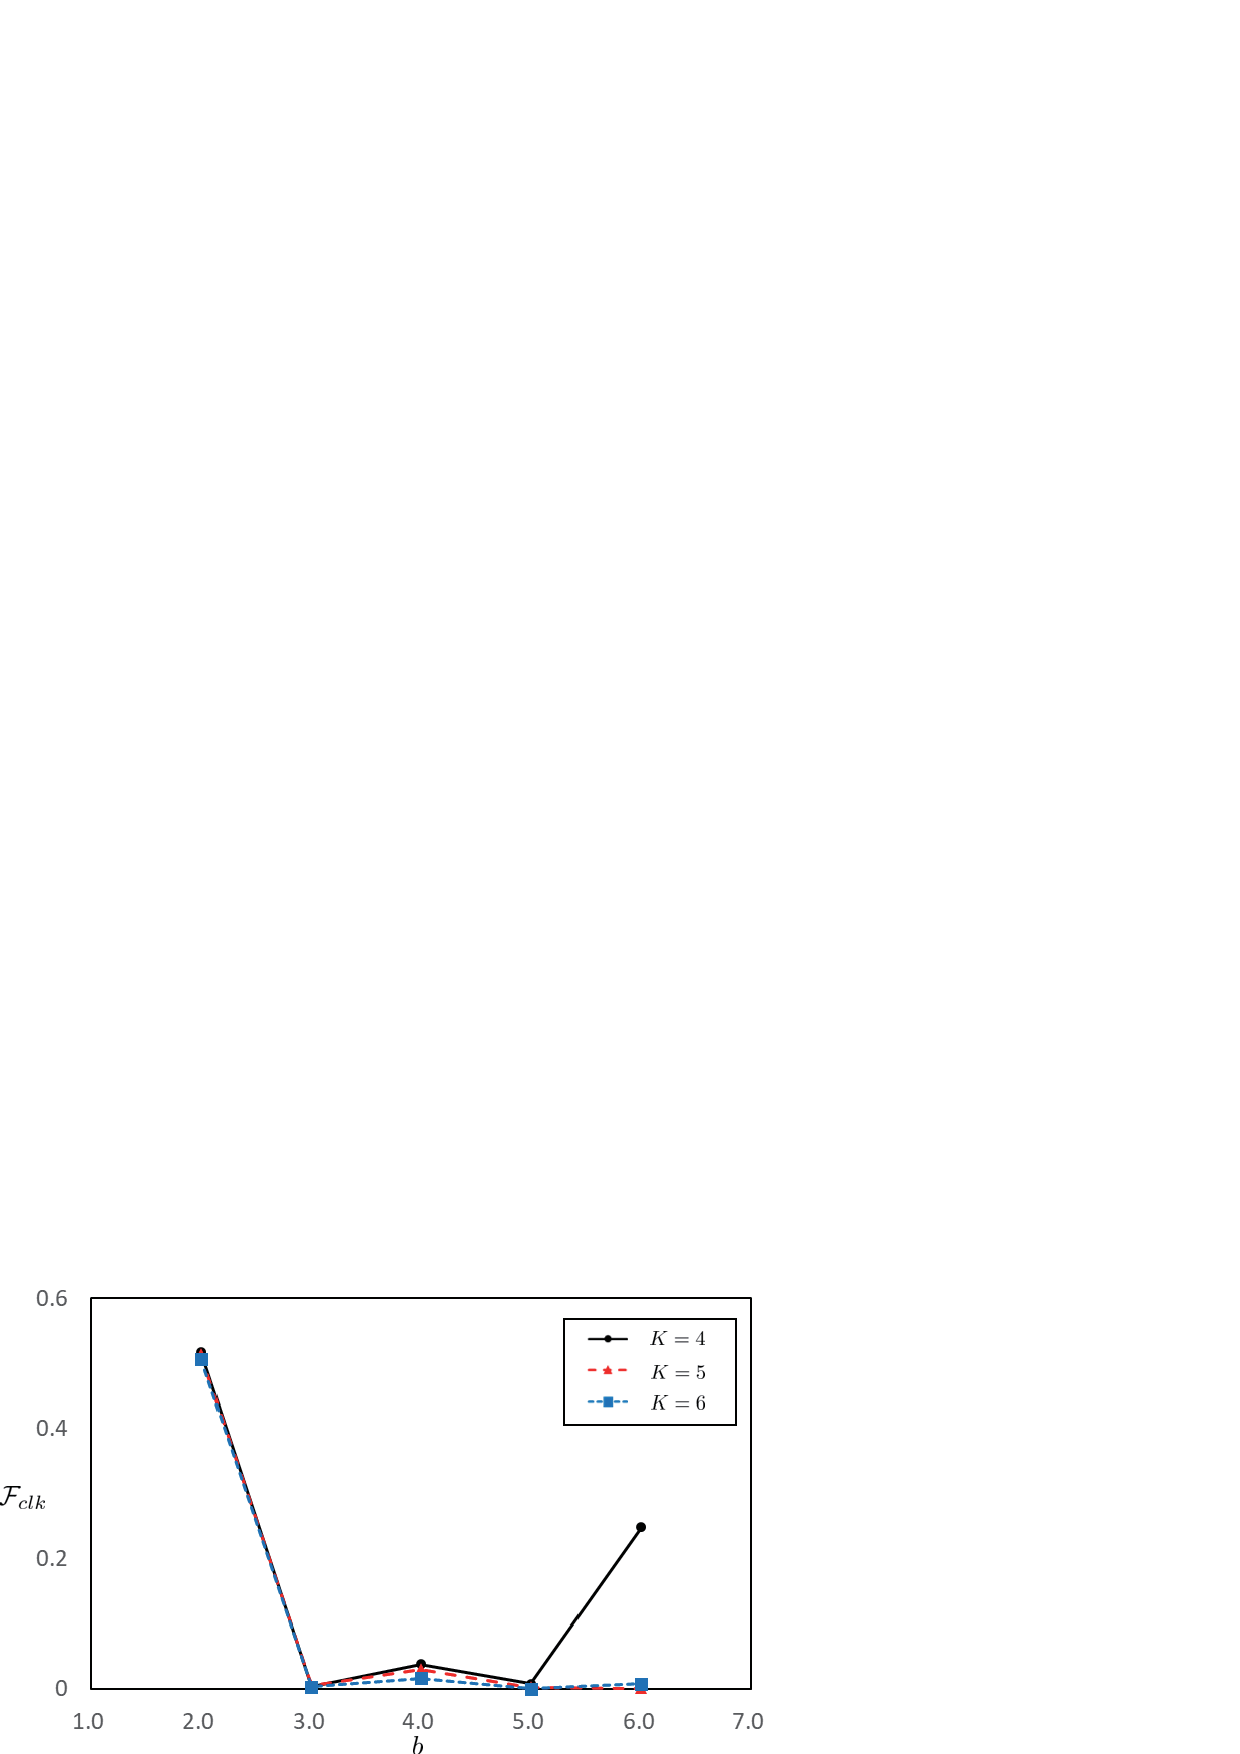
\includegraphics[scale=0.35]{fig/fig5.pdf}
\vspace{-10pt}
\caption{Hyperparameter analysis. (a) Study of $\alpha$ on MSVD-QA, which controls the equivariant mixing ratio by $\lambda_0\sim\text{Beta}(\alpha,\alpha)$. Performance of two EIGV enhanced models --- HGA (top) and MSPAN (bottom) are reported, alongside the SoTA backbone and mixup augmented performances.  
(b) Study on the impact of the negative sample number N, where EIGV with two backbones (\ie MSPAN and HGA) on two benchmark datasets (NExT-QA and MSVD-QA) are reported.}
\vspace{-10pt}
\label{fig:neg}
\end{figure}
\section{Related Work}
\label{sec:related}

\begin{figure*}[t]
  \centering
%   \setlength{\abovecaptionskip}{0.cm}
  \includegraphics[width=0.97\textwidth]{fig/case.pdf}
 	\vspace{-13pt}
  \caption{Visualization of discovered grounding rationale. Each row comes with a video instance and two questions that target at different scene.  The \textcolor[rgb]{0,0.5,0}{green} and \textcolor[RGB]{225,152,150}{pink} windows indicate the rationales for the corresponding questions.}
  \label{fig:case-study}
 	\vspace{-10pt}
\end{figure*}

\vspace{5pt}
\noindent\textbf{Video Question Answering.}
Established to answer the question in dynamic visual content, VideoQA is bred through the task of ImageQA but has broadened its definition by assembling a temporal dimension. 
%
To make the task intriguing, the VideoQA benchmark has gone beyond the problem of description \cite{DBLP:conf/mm/XuZX0Z0Z17} and built several datasets to challenge temporal reasoning and even causal reflection \cite{DBLP:conf/cvpr/XiaoSYC21}. 
%
As a result, VideoQA has experienced an aggressive expansion in the architecture design. 
% 
Chronologically, early efforts tend to enact alignment through cross-modal attention \cite{zeng2016leveraging,li2019beyond} or enhanced memory design \cite{gao2018motionappearance, DBLP:conf/mm/XuZX0Z0Z17, fan2019heterogeneous}, while more recent works leverage the expressiveness of the graph neural network and perform the relation reasoning as node propagation \cite{jiang2020reasoning, DBLP:conf/mm/PengYBW21} or graph alignment \cite{park2021bridge}. 
%
In addition, current designs modify the representation of video and manipulate the temporal sequence from a hierarchical angle. Following this line, HCRN \cite{le2021hierarchical} first came out with the conditional relation module as building blocks that operate through different video intervals, whereas  HOSTR and PGAT made their advancement by incorporating visual content from different granularity. MSPAN, however, established cross-scale feature interaction on top of the hierarchy.
%
Despite effective, their intrinsic rationale has long been overlooked. To the best of our knowledge, EIGV is the first work that probes intrinsic interpretation. 

\vspace{5pt}
\noindent\textbf{Invariant Learning.}
% Given a encoder $f(\cdot)$ and input $x$, a representation $f(x)$ is equivariant to operation $G$, if $\forall x : f(G(x)) = T(G(x))$ ; Likewise, the property of invariance is defined as $\forall x : f(G(x)) = f(x)$. 
Given a encoder $f(\cdot)$ and input $x$, a representation $f(x)$ is invariant to operation $T$, if $\forall x : f(G(x)) = f(x)$. 
%
In practice, this invariant property has a long history in presenting visual content (\eg HOG \cite{DBLP:conf/mmm/HuangTHTJ11}), which has recently been renovated by deep learning in form of risk minimization. As its most prevailing form, IRM \cite{arjovsky2020invariant} fosters this philosophy by posing an environment invariant prior and discovering the underlying causal pattern by reducing cross-environment variance.   
% .that remains stable across different environments.
Different from previous studies that create environment via inductive re-grouping \cite{DBLP:conf/cvpr/AndersonWTB0S0G18} or adversarial inference \cite{DBLP:conf/icml/CreagerJZ21,wang2021causal, wang2022causal,wang2021clicks}, our method conducts causal intervention that perturbs the original sample distribution to form a new one.
\lyc{The most relvant work is \cite{Li_2022_CVPR}, where an invariant framework is introduced as a model-agnostic framework. However, EIGV gains better generalization ability by marrying equivariance as complementary learning principle.}
% Specifically, the discovery of  rationale implies two requirements on the partition:

\vspace{5pt}
\noindent\textbf{Visual Interpretability}
Machine interpretability can be achieved in various methods, such as clustering \cite{monnier2020dticlustering} or disentanglement \cite{shen2020interfacegan}. Our design can be vested in the category of attribution discovery, which investigates the contribution of different input elements toward the prediction. 
Based on whether the prediction and interpretation are yielded simultaneously, two categories are further defined: 1) post-hoc methods that generated the interpretation after prediction, such as backpropagation methods (\eg grad-CAM \cite{DBLP:conf/iccv/SelvarajuCDVPB17}). 2) self-interpretable method that cast prediction and interpretation at the same stage.
%
Unlike the post-hoc method that traces the interpretative clue from the output of the black-box, the self-interpretable model builds a transparency model via methods such as prototype generation \cite{DBLP:journals/corr/abs-1806-10574} or structural delineation \cite{wu2022dir}. 
%
In fact, previous works tend to focus on static image. EIGV, however, approaches the video interpretation in a multi-modal situation. 

\vspace{-5pt}
\section{conclusion}
\label{sec:conclusion}
In this paper, we present EIGV --- a model-agnostic explainer, that empowers the SoTA VideoQA model with intrinsic interpretability. In the light of the causality, we formulate our learning principles --- causal-equivariance and environment-invariance by incorporating three constituents, the grounding indicator, the intervener, and the disruptor, which manage a robust rationale discovery. Experiments across three benchmarks validate EIGV's fulfillment in both interpretation and accuracy.

% In addition to the technical advantages, we discuss possible refinements to improve the current design. Unlike some SoTAs that utilize object-level features (\eg HOSTR \cite{dang2021hierarchical} and PGAT \cite{DBLP:conf/mm/PengYBW21}), EIVG merely takes advantage of clip-level representation. Although the architecture of the backbone model is beyond the scope of this work, we anticipate that a fine-grained interpretation at the entity level will strengthen the current EIGV design.
% \section{Limitation and Complexity}
\label{section:limits}
\lyc{In addition to the technical advantages, we discuss possible limits of the current design. Unlike some SoTAs that utilize object-level features (\eg HOSTR \cite{dang2021hierarchical} and PGAT \cite{DBLP:conf/mm/PengYBW21}), EIVG merely takes advantage of clip-level representation. Although the architecture of the backbone model is beyond the scope of this work, we anticipate that a fine-grained interpretation at the entity level will strengthen the current EIGV design.
% 2) Current intervention strategy can possibly threaten the causal prediction by introducing context with new shortcuts. Since the scene intervener sample context stratification in a random manner, there is a slight chance to draw an undesired substitute that nested with strong static relation towards  a wrong answer, thus inducing a false prediction.
In terms of complexity, we run all experiments on NVIDIA Tesla V100 GPU, where our algorithm matched equally with the corresponding baseline.  For comparison, the backbone MSPAN model is trained for 1.5 hours till convergence on NExT-QA, whereas EIGV 
takes 1.6 hours.
}

%%
%% The next two lines define the bibliography style to be used, and
%% the bibliography file.

\bibliographystyle{ACM-Reference-Format}
\balance
\bibliography{sample-base}

%%
%% If your work has an appendix, this is the place to put it.
% \appendix


\end{sloppypar}
\end{document}
\endinput
%%
%% End of file `sample-sigconf.tex'.

\section{VideoQA Reformulation}
\label{sec:reformulation}

\wx{Here we argue that disclosing ``Which part of the video is critical to answering the question?'' is the key to presenting the visual-linguistic alignment explicitly.
To this end, we take a causal \cite{pearl2009causal} look at the reasoning process of VideoQA, then formalize it as a Structure Causal Model (SCM) \cite{pearl2016causal} by investigating the causal relationships among five variables: input video $V$, question $Q$, causal scene $C$, environment scene $E$, ground-truth answer $A$.
% Moreover, we analyze the conventional ERM scheme's limitations on
}

% Discovering the grounding rationale for faithful prediction requires careful inspection of the data generating process. In light of the causal theory \cite{pearl2016causal}, we revisit the formation of VideoQA models, then formalize them as a Structure Causal Model (SCM) \cite{pearl2009causal}  by investigating causality among five variables: input video $V$, question $Q$, causal scene $C$, environment scene $E$, ground-truth answer $A$.

\subsection{Causal Graph of VideoQA}\label{sec:causal-view}
\wx{Figure \ref{fig:scm} illustrates the causal graph, where each link depicts the cause-effect relationship between two variables:
\begin{itemize}[leftmargin=*]
    \item $Q\to C, E \gets V$. Given the question of interest $Q$, the video $V$ can be partitioned into two parts: (1) the causal scene $C$, which retains the question-critical information and naturally serves as the rationale for answering, (2) the environment scene $E$, which gathers the cues irrelevant to the question-answering. For example, to answering ``What is the girl doing?'' in Figure \ref{fig:overview}, $C$ should be the first two clips describing the ``girl-riding on-horse'' scene, while $E$ should be the last clip about the ``meadow'' scene. Moreover, the varying semantics of different questions will emphasize different $C$.
    \item $Q\rightarrow A \leftarrow C$. The visual knowledge in the causal scene $C$ and the linguistic semantics in the question $Q$ collaborate together to determine the answer $A$. Furthermore, this path, which presents the visual-linguistic alignment, internally interprets the reasoning.
    \item $E\dashleftarrow\dashrightarrow C$. The dashed arrow sketches additional probabilistic dependencies \cite{reason:Pearl09a} between $C$ and $E$, which typically arise from selection bias \cite{DBLP:conf/cvpr/TorralbaE11}. For example, the ``meadow'' scene is frequently collected as a common environment for the ``horse-riding'' scene. 
\end{itemize}}


\subsection{Beyond ERM}
\lyc{With inspections on prior VideoQA studies, we investigate their inability to distinguish the causal and non-causal effects of scenes.
Specifically, in conventional VideoQA models, video and question are directly paired together to model their interaction and approach the golden answer, consequently.
Inevitably, taking video as a whole leaves the contributions of scenes untouched, thus failing to differentiate $C$ from $E$ and forgoing their function divergence towards the answer.
Worse still, ERM enforces these models to blindly capture the statistical correlations between the video-question pairs and answers.
As such, the visual-linguistic alignment hinges easily on the spurious correlations between $E$ and $A$, owing to the backdoor paths \cite{pearl2016causal}, which hinders the generalization of models \cite{niu2020counterfactual,wu2022dir}.
Therefore, identifying the causal scene $C$ is the critical to addressing these limitations.}



\begin{figure}[t]
\centering
\includegraphics[scale=0.3]{fig/scm.pdf}
\vspace{-5pt}
\caption{Causal Graph of VideoQA}
\vspace{-10pt}
\label{fig:scm}
\end{figure}

\section{Experiment}
\label{sec:experiment}

In this section, we show the experimental results to answer the following research questions.
\begin{itemize}[leftmargin=*]
\item \textbf{RQ1} How effective is EIGV in discovering the causal pattern and improving the model generalization across different settings?
\item \textbf{RQ2} How does the sub-module and feature setting contribute to the performance?
\item \textbf{RQ3} What pattern does EIGV capture in rationale discovery?
\end{itemize}

\subsection{Settings}

\vspace{5pt}
\noindent \textbf{Datasets.} We conduct experiments on three benchmark datasets that challenge the model's reasoning capacity from different aspects: 
\textbf{MSVD-QA}  \cite{DBLP:conf/mm/XuZX0Z0Z17} and \textbf{MSRVTT-QA} \cite{DBLP:conf/mm/XuZX0Z0Z17} mainly emphasize the recognition ability by asking the descriptive questions, where 50K and 243K question-answer pairs are automatically generated from the human-labeled video captions, respectively.
\textbf{NExT-QA} \cite{DBLP:conf/cvpr/XiaoSYC21} pinpoints the causal and temporal relations among objects in the video. It contains 47.7K questions with answers in the form of multi-choice, which are manually annotated from 5.4K videos.

\vspace{5pt}
\noindent\textbf{Baseline.} We validate the effectiveness of EIGV across backbone VideoQA models of three kinds: 
1) \textbf{Memory-based} methods that foster a storage of input sequence via auxiliary memory design, such as AMU \cite{DBLP:conf/mm/XuZX0Z0Z17}, HME \cite{fan2019heterogeneous} and Co-Mem \cite{gao2018motionappearance}.
2) \textbf{Graph-based} methods that leverage the expressiveness of graph network to model the interaction between visual and language elements, which involves methods like L-GCN \cite{huang2020locationaware}, B2A  \cite{park2021bridge} and HGA \cite{jiang2020reasoning}. 
3) \textbf{Hierarchy-based} methods include HCRN \cite{le2021hierarchical}, PGAT \cite{DBLP:conf/mm/PengYBW21}, HOSTR \cite{dang2021hierarchical}, MSPAN \cite{DBLP:conf/acl/GuoZJ0L20} and HQGA \cite{xiao2021video}. In common, they exploit the multi-granularity nature of visual elements and realize the hierarchical reasoning via bottom-up architecture. 
In Specific, we test the generalization of EIGV by marrying our learning principles to three backbones of different categories: memory-based Co-Mem \cite{gao2018motionappearance}, graph-based HGA \cite{jiang2020reasoning} and hierarchy-based MSPAN \cite{DBLP:conf/acl/GuoZJ0L20}. 

\vspace{5pt}
\noindent \textbf{Implementation Detail.} 
For input representation, we encode the video instance as a sequence of $K$=16 clips, where each clip is represented as a combination of appearance and motion features extracted from the pre-trained ResNet-152 and 3D ResNeXt-101. For the linguistic feature, we follow \cite{DBLP:conf/cvpr/XiaoSYC21} and obtain the contextualized word representation using the fine-tuned BERT model. In the hyper-parameters setting, we set $d=512$ for cross-modal alignment, then train the model for 80 epochs with an initial learning rate of 5e-5.  During optimization, EIGV is trained with Adam optimizer and we decay the learning rate when validation stops improving for 5 epochs. The balance ratio $\beta$ is set to 0.75.
%for open-set QA and 0.025 for multi-choice QA. 

\subsection{Main Result (RQ1)}
\def\year{2019}\relax
%File: formatting-instruction.tex
\documentclass[letterpaper]{article} %DO NOT CHANGE THIS
% \usepackage{aaai19}  %Required
\usepackage{arXiv}  % for arXiv  <<<<<<<<<<<<<<<<<<<<<<<<<<<<<<<<<<<<<<<<<<<<<<<<<<<
\usepackage{times}  %Required
\usepackage{helvet}  %Required
\usepackage{courier}  %Required
\usepackage{url}  %Required
\usepackage{graphicx}  %Required
\frenchspacing  %Required
\setlength{\pdfpagewidth}{8.5in}  %Required
\setlength{\pdfpageheight}{11in}  %Required

% DY added
% \usepackage[final]{hyperref}
\usepackage{multirow}
\usepackage{amsmath}
\usepackage{subfig}
% \usepackage{subcaption}

% \usepackage{caption}
\usepackage{multirow}
\usepackage{bbm}

\usepackage{xcolor}
\usepackage{colortbl}
\usepackage{array}
\usepackage{pifont}
\usepackage{booktabs}


%PDF Info Is Required:
  \pdfinfo{
/Title (Utilizing Class Information for Deep Network Representation Shaping)
/Author (Daeyoung Choi, Wonjong Rhee)}
\setcounter{secnumdepth}{0}  
% \setcounter{secnumdepth}{2} % for arXiv <<<<<<<<<<<<<<<<<<<<<<<<<<<<<<<<<<<<<<<<<<<<<<<<<<<

\begin{document}
% The file aaai.sty is the style file for AAAI Press 
% proceedings, working notes, and technical reports.
%
\title{Utilizing Class Information for Deep Network Representation Shaping}

\author{Daeyoung Choi\thanks{Authors contributed equally.} and Wonjong Rhee\footnotemark[1] \\
Department of Transdisciplinary Studies\\
Seoul National University\\
Seoul, 08826, South Korea \\
\texttt{\{choid, wrhee\}@snu.ac.kr} 
}
\maketitle
\begin{abstract}
Statistical characteristics of deep network representations, such as sparsity and correlation, are known to be relevant to the performance and interpretability of deep learning. When a statistical characteristic is desired, often an adequate regularizer can be designed and applied during the training phase. Typically, such a regularizer aims to manipulate a statistical characteristic over all classes together. For classification tasks, however, it might be advantageous to enforce the desired characteristic per class such that different classes can be better distinguished. Motivated by the idea, we design two class-wise regularizers that explicitly utilize class information: class-wise Covariance Regularizer (cw-CR) and class-wise Variance Regularizer (cw-VR). cw-CR targets to reduce the covariance of representations calculated from the same class samples for encouraging feature independence. cw-VR is similar, but variance instead of covariance is targeted to improve feature compactness. For the sake of completeness, their counterparts without using class information, Covariance Regularizer (CR) and Variance Regularizer (VR), are considered together. The four regularizers are conceptually simple and computationally very efficient, and the visualization shows that the regularizers indeed perform distinct representation shaping. In terms of classification performance, significant improvements over the baseline and L1/L2 weight regularization methods were found for 21 out of 22 tasks over popular benchmark datasets. In particular, cw-VR achieved the best performance for 13 tasks including ResNet-32/110. 
\end{abstract}


%=============================================
% #Introduction
%=============================================

\section{Introduction}
%

\begin{figure}[t]
% \vskip 0.1in
\centering
\centerline{\includegraphics[width=8.25cm]{mnist_none_hist_scatter.pdf}}
\caption{
% \small{
A single unit's activation histogram (upper three plots) and two randomly chosen units' activation scatter plots (lower three plots) for MNIST. For a 6-layer Multilayer Perceptron (MLP), the fifth layer's representation vectors calculated using 10,000 test samples were used to generate the plots. For the baseline model, a substantial overlap among different classes can be observed at the time of initialization as shown in (a). Even after 50 epochs of training, still, a substantial overlap can be observed as shown in (b). When class information is used to regularize the representation shapes, the overlap is significantly reduced as shown in (c). Note that a slight correlation between each pair of classes can be observed in the scatter plot of (b), but not in that of (c) due to the use of cw-CR. The figures are best viewed in color.
% }
}
\label{fig:mnist_none_hist_scatter}
% \vskip -0.3in
\end{figure}

For deep learning, a variety of regularization techniques have been developed by focusing on the \textit{weight parameters}. A classic example is the use of L2 \cite{hoerl1970ridge} and L1 \cite{tibshirani1996regression} weight regularizers. They have been popular because they are easy to use, computationally light, and often result in performance enhancements. Another example is the parameter sharing technique that enforces the same weight values as in the Convolutional Neural Networks (CNNs).  
Regularization techniques that focus on the \textit{representation} (the activations of the units in a deep network), however, have been less popular even though the performance of deep learning is known to depend on the learned representation heavily. 

For representation shaping (regularization), some of the promising methods for performance and interpretability include \cite{glorot2011deep,cogswell2015reducing,liao2016learning}.
\cite{glorot2011deep} considers increasing representational sparsity, \cite{cogswell2015reducing} focuses on reducing covariance among hidden units, and \cite{liao2016learning} forces parsimonious representations using k-means style clustering. While all of them are effective representation regularizers, none of them explicitly use class information for the regularization. A few recent works \cite{wen2016discriminative,belharbi2017neural,yang2018robust} do utilize class information, and their approaches are based on \textit{hidden layer activation vectors}. The method of \cite{belharbi2017neural} is computationally expensive because pair-wise dissimilarities need to be calculated among the same class samples in each mini-batch. 

In this work, two computationally light representation regularizers, cw-CR (class-wise Covariance Regularizer) and cw-VR (class-wise Variance Regularizer), that utilize class information are introduced and studied. We came up with the design ideas by observing typical histograms and scatter plots of deep networks as shown in Figure \ref{fig:mnist_none_hist_scatter}. In Figure \ref{fig:mnist_none_hist_scatter} (b), different classes substantially overlap even after the training is complete. If we directly use class information in regularization, as opposed to using it only for cross-entropy cost calculation, we can specifically reduce overlaps or pursue a desired representation characteristic. An example of cw-CR reducing class-wise covariance is shown in Figure \ref{fig:mnist_none_hist_scatter} (c), and later we will show that cw-VR can notably reduce class-wise variance resulting in minimal overlaps. The two class-wise regularizers are very simple and computationally efficient, and therefore can be easily used as L1 or L2 weight regularizers that are very popular. 

% our contributions
\subsection{Our Contributions}
The contributions of this work can be summarized as follows.

\subsubsection{Introduction of three new representation regularizers} 
We introduce two representation regularizers that utilize class information. cw-CR and cw-VR reduce per-class covariance and variance, respectively. In this work, their penalty loss functions are defined, and their gradients are analyzed and interpreted. Also, we investigate VR that is cw-VR's all-class counterpart. Intuitively, reducing the variance of each unit's activations does not make sense unless it is applied per class, but we have tried VR for the sake of completeness and found that VR is useful for performance enhancement. cw-CR's all-class counterpart, CR, is analyzed as well, but CR turns out to be the same as DeCov that was already studied in-depth in \cite{cogswell2015reducing}. 

\subsubsection{Performance improvement with the new representation regularizers}
Rather than trying to find a single case of beating the state-of-the-art record, we performed an extensive set of experiments on the most popular datasets (MNIST, CIFAR-10, CIFAR-100) and architectures (MLP, CNN). Additionally, ResNet \cite{he2016deep} was tested as an example of a sophisticated network, and an image reconstruction task using autoencoder was tested as an example of a different type of task. We have tested a variety of scenarios with different optimizers, number of classes, network size, and data size. The results show that our representation regularizers outperform the baseline (no regularizer) and L1/L2 weight regularizers for almost all the scenarios that we have tested. More importantly, class-wise regularizers (cw-CR, cw-VR) usually outperformed their all-class counterparts (CR, VR). Typically cw-VR was the best performing regularizer and achieved the best performance for the autoencoder task, too.

\subsubsection{Effects of representation regularization}
Through visualizations and quantitative analyses, we show that the new representation regularizers indeed shape representations in the ways that we have intended. The quantitative analysis of representation characteristics, however, indicates that each regularizer affects multiple representation characteristics together and therefore the regularizers cannot be used to control a single representation characteristic without at least mildly affecting some other representation characteristics. 


%=============================================
% #Related Works
%=============================================

\section{Related Works}

\subsection{Regularization for Deep Learning}
%
The classic regularizers apply L2 \cite{hoerl1970ridge} and L1 \cite{tibshirani1996regression} 
penalties to the \textit{weights} of models, and they are widely used for Deep Neural Networks (DNNs) as well. 
%
\cite{wen2016learning} extended L1 regularizers by using group lasso to regularize 
the structures of DNN (i.e., filters, channels, filter shapes, and layer depth).
%
\cite{srivastava2014dropout} devised dropout that randomly applies activation masking 
over the units.
%
While dropout is applied in a multiplicative manner, \cite{glorot2011deep} used L1 penalty 
regularization on the activations to encourage sparse representations.
%
XCov proposed by \cite{cheung2014discovering} minimizes the covariance between 
autoencoding units and label encoding units of the same layer such that 
representations can be disentangled.  
%
Batch normalization (BN) proposed by \cite{ioffe2015batch} exploits mini-batch statistics 
to normalize activations. It was developed to accelerate training speed by preventing 
internal covariate shift, but it was also found to be a useful regularizer.
%
In line with batch normalization, weight normalization, developed by \cite{salimans2016weight}, 
uses mini-batch statistics to normalize weight vectors. 
%
Layer normalization proposed by \cite{ba2016layer} is a RNN version of batch normalization,
where they compute the mean and variance used for normalization from all of the summed
inputs to the units in a layer on a single training case.
%
There are many other publications on regularization techniques for deep learning,
but we still do not fully understand how they really affect the performance.  
Recent work by \cite{zhang2016understanding}
shows that the traditional concept of controlling generalization error by regularizing the effective capacity does not apply to the modern DNNs. 


\subsection{Penalty Regularization on Representations}
Some of the existing regularization methods explicitly shape representations by adopting a penalty regularization term.
%
DeCov \cite{cogswell2015reducing} is a penalty regularizer that minimizes the off-diagonals of a layer's representation covariance matrix. DeCov reduces co-adaptation of a layer's units by encouraging the units to be decorrelated. In this work, 
it is called as CR (Covariance Regularizer) for consistent naming.
%
A recent work \cite{liao2016learning} used a clustering based regularization that encourages parsimonious representations. In their work, similar representations in sample, spatial, and channel dimensions are clustered and used for regularization such that similar representations are encouraged to become even more similar. While their work can be applied to unsupervised as well as supervised tasks, our work utilizes a much simpler and computationally efficient method of directly using class labels during training to avoid k-means like clustering. 

\subsection{Class-wise Learning}
True class information has been rarely used directly for regularization methods.
Traditionally, the class information has been used only for evaluating the correctness of
predictions and the relevant cost function terms. Some of the recent works, however, 
have adopted the class-wise concept in more sophisticated ways. In those works, 
class information is used as a switch or for emphasizing the discriminative aspects over different classes. 
%
As an example, \cite{li2008kernel} proposed a kernel learning method using class information to model the manifold structure. They modify locality preserving projection to be class dependent. \cite{jiang2011learning} 
added label consistent regularizers for learning a discriminative dictionary. 
%
\cite{wen2016discriminative} developed a regularizer called center loss that reduces the activation vector distance between representations and their corresponding class centers for face recognition tasks.
%
\cite{yang2018robust} designed a loss function named prototype loss that improves representation's intra-class compactness for enhancing the robustness of CNN.
%
Another recent work by \cite{belharbi2017neural} directly uses class labels to encourage similar representations per class as in our work, but it is computationally heavy as explained earlier.  
Besides the pair-wise computation, two optimizers are used for handling the supervised loss term and the hint term separately. 
%
Class information is used for autoencoder tasks as well. \cite{shi2016learning} implicitly reduced the intra-class variation of reconstructed samples by minimizing pair-wise distances among same class samples.
%
Like the strategies listed above, our cw-VR and cw-CR use class-wise information to control the statistical characteristics of representations. However, our methods are simple because only one optimizer is used, and computationally efficient because pair-wise computation is not required.


%=============================================
% #Class-wise Representation Regularizers
%=============================================

\section{Class-wise Representation Regularizers: cw-CR and cw-VR}

In this section, we first present basic statistics of representations. Then, three representation regularizers, cw-CR, cw-VR, and VR are introduced with their penalty loss functions and gradients. Interpretations of the loss functions and gradients are provided as well. 

\subsection{Basic Statistics of Representations}
\label{subsection:stats}
For the layer $l$, the output activation vector of the layer is defined as 
$\mathbf{z}_l = \max(\mathbf{W}^\top_l \mathbf{z}_{l-1} + \mathbf{b}_l, 0)$ using Rectified Linear Unit (ReLU)
activation function. Because we will be focusing on the layer $l$ for most of the explanations, 
we drop the layer index. 
Then, $z_i$ is the $i^{th}$ element of $\mathbf{z}$ (i.e. activation of $i^{th}$ unit). 
%  ,and $w_{ki}$ is the $(k,i)$ element of $\mathbf{W}$. 

To use statistical properties of representations, we define mean of unit $i$, $\mu_i$, and covariance 
between unit $i$ and unit $j$, $\textit{c}_{i,j}$, using the $N$ samples in each mini-batch. 
\begin{align}
    \mu_i &= \frac{1}{N} \sum_n z_{i,n}  \label{eq:mean}  \\
    \textit{c}_{i,j} &= \frac{1}{N} \sum_n (z_{i,n} - \mu_i)(z_{j,n} - \mu_j) \label{eq:covariance}
\end{align}
Here, $z_{i,n}$ is the activation of unit $i$ for $n^{th}$ sample in the mini-batch.  
From equation (\ref{eq:covariance}), variance of $i$ unit can be written as the following. 
\begin{align}
    \textit{v}_{i} &= \textit{c}_{i,i} \label{eq:variance}
\end{align}
When class-wise statistics need to be considered, we choose a single label $k$ from $K$ labels
and evaluate mean, covariance, and variance using only the data samples with true label $k$
in the mini-batch. 
\begin{align}
    \mu_i^k &= \frac{1}{|S_k|} \sum_{n \in S_k} z_{i,n} \label{eq:mean_cw} \\
    \textit{c}_{i,j}^k &= \frac{1}{|S_k|} \sum_{n \in S_k} (z_{i,n} - \mu_i^k)(z_{j,n} - \mu_j^k) \label{eq:covariance_cw}  \\  
    \textit{v}_{i}^k &= \textit{c}_{i,i}^k   \label{eq:variance_cw}
\end{align}
Here, $S_k$ is the set containing indexes of the samples whose true label is $k$, 
and $|S_k|$ is the cardinality of the set $S_k$.

\begin{table*}[t]
\caption{Penalty loss functions and gradients of the representation regularizers. All the penalty loss functions are normalized with the number of units ($I$) and the number of classes ($K$) such that the value of $\lambda$ can have a consistent meaning. CR and cw-CR are standardized using the number of distinct covariance combinations.}
% \vskip 0.15in
\centering
% \begin{small}
% \setlength{\tabcolsep}{8pt} % Default value: 6pt
% \renewcommand{\arraystretch}{2} % Default value: 1
\begin{tabular}{rlrl}
		\hline
		\multicolumn{2}{c}{Penalty loss function}  & \multicolumn{2}{c}{Gradient}  \\ \hline
		$\displaystyle{\Omega}_{CR}$ & $\displaystyle=\frac{2}{I(I-1)}\sum_{i\neq j} (c_{i,j})^{2} $    & $\displaystyle\frac{\partial{{\Omega}_{CR}}}{\partial{z_{i,n}}}$ & $\displaystyle=\frac{4}{NI(I-1)}\sum_{j\neq{i}}^{}{c_{i,j}(z_{j,n}-\mu_{j}})$  \\ 
		
		$\displaystyle{\Omega}_{cw{\text -}CR}$ & $\displaystyle=\frac{2}{KI(I-1)}\sum_k \sum_{i\neq j} (c_{i,j}^{k})^{2} $   & $\displaystyle\frac{\partial{{\Omega}_{cw{\text-}CR}}}{\partial{z_{i,n}}}$ & $\displaystyle=\frac{4}{KI(I-1)|S_k|}\sum_{j\neq{i}}^{}{c_{i,j}^{k}(z_{j,n}-\mu_{j}^{k}}),  n \in S_k$  \\ 
		
		$\displaystyle{\Omega}_{VR}$ & $\displaystyle=\frac{1}{I}\sum_i v_{i}$                                               & $\displaystyle\frac{\partial{{\Omega}_{VR}}}{\partial{z_{i,n}}}$ & $\displaystyle=\frac{2}{NI}(z_{i,n}-\mu_{i})$  \\
		
		$\displaystyle{\Omega}_{cw{\text -}VR}$ & $\displaystyle=\frac{1}{K I}\sum_k \sum_i v_{i}^k $                        & $\displaystyle\frac{\partial{{\Omega}_{cw{\text -}VR}}}{\partial{{z}_{i,n}}}$ & $\displaystyle =\frac{2}{KI|S_k|}({z}_{i,n}-{\mu}_{i}^{k}), n \in S_k$  \\ \hline
	\end{tabular}
% \end{small}
\label{table:loss_function}
% \vskip -0.2in
\end{table*}

\subsection{cw-CR}
cw-CR uses off-diagonal terms of the mini-batch covariance matrix of activations per class as the penalty term: ${\Omega}_{cw{\text -}CR}=\sum_k \sum_{i\neq j} (c_{i,j}^{k})^{2}$. This term is added to the original cost function $J$, and the total cost function $\widetilde{J}$ can be denoted as  
\begin{align}
    \widetilde{J}=J+\lambda{\Omega}_{cw{\text -}CR}(\mathbf{z}),
\end{align}
where $\lambda$ is the penalty loss weight ($\lambda \in [0, \infty)$). The penalty loss weight balances between the original cost function $J$ and the penalty loss term $\Omega$. When $\lambda$ is equal to zero, $\widetilde{J}$ is the same as $J$, and cw-CR does not influence the network. When $\lambda$ is a positive number, the network is regularized by cw-CR, and the performance is affected. In practice, we have observed that deep networks with too large $\lambda$ cannot be trained at all.

\subsection{cw-VR}
A very intuitive way of enforcing distinguished representations per class is to maximize the inter-class distances in the representation space. 
%However, such a distance maximizer turns out to be difficult to implement as a penalty loss function because the cost function needs to be maximized and not minimized. 
%We implemented the idea and applied the regularizer, but the optimization became unstable (failed to converge). 
%Inter-class distance needs to be maximized. To include the penalty term to the cost function (that needs to be minimized), we tried inversion and multiplication by -1. Both caused the optimization to diverge. 
Because inter-class needs to be maximized, the corresponding penalty term can be inverted or multiplied by -1 before it is minimized with the original cost function. 
We tried such approaches, but the optimization became unstable (failed to converge).
%
An alternative way is to reduce intra-class (same-class) variance. By applying this idea, the penalty loss term of cw-VR can be formulated as ${\Omega}_{cw{\text -}VR}=\sum_k \sum_i v_{i}^k$. 

With the design of cw-VR, we naturally invented VR that is the all-class counterpart of cw-VR. VR minimizes the activation variance of each unit, and it is mostly the same as cw-VR except for not using the class information. We expected VR to hurt the performance of deep networks because it encourages all classes to have similar representation in each unit. VR, however, turned out to be effective and useful for performance enhancement. We provide a possible explanation in the Experiments section. 

\subsection{Penalty Loss Functions and Gradients}

The penalty loss functions of cw-CR and cw-VR are similar to CR and VR, respectively, except that the values are calculated for each class using the mini-batch samples with the same class label. Also, gradients of CR and cw-CR are related to those of VR and cw-VR as shown in Table \ref{table:loss_function}. We investigate more details of the equations in the following.

\subsubsection{Interpretation of the gradients}
Among the gradient equations shown in Table \ref{table:loss_function}, the easiest to understand is VR's gradient. It contains the term ${z}_{i,n}-{\mu}_{i}$, indicating that the representation ${z}_{i,n}$ of each sample $n$ is encouraged to become closer to the mean activation ${\mu}_{i}$. In this way, each unit's variance can be reduced. For cw-VR, the equation contains ${z}_{i,n}-{\mu}_{i}^{k}$ instead of ${z}_{i,n}-{\mu}_{i}$. Therefore the representation ${z}_{i,n}$ of a class $k$ sample is encouraged to become closer to the \textit{class} mean activation ${\mu}_{i}^{k}$. Clearly, the variance reduction is applied per class by cw-VR. 

For CR, the equation is less straightforward. As explained in \cite{cogswell2015reducing}, a possible interpretation is that the covariance term $c_{i,j}$ is encouraged to be reduced where $z_{j,n}-\mu_j$ acts as the weight. But, another possible interpretation is that $z_{j,n}$ is encouraged to become closer to $\mu_j$ just as in the case of VR, where $c_{i,j}$ acts as the weight. Note that VR's mechanism is straightforward where each unit's variance is directly addressed in the gradient equation of activation $i$, but CR's mechanism is slightly complicated where all variances over all activations of $j$ ($j=1,...,I$, where $j \neq i$) are collectively addressed through the summation terms over all $j$ ($j=1,...,I$, where $j \neq i$). Thus, one can interpret CR as a hybrid regularizer that wants either or both of covariance and variance to be reduced. This can be the reason why the visualizations of CR and VR are similar as will be shown in Figure \ref{fig:representation} later. 

For cw-CR, it can be interpreted similarly. As in the relationship between VR and cw-VR, cw-CR is the class-wise counterpart of CR and it can be confirmed in the gradient equation: cw-CR has $c_{i,j}^k({z}_{j,n}-{\mu}_{j}^{k})$ instead of $c_{i,j}({z}_{j,n}-{\mu}_{j})$. As in our explanation of CR, cw-CR can also be interpreted as trying to reduce either or both of covariance and variance. The visualizations of cw-CR and cw-VR turn out to be similar as well. 

The interpretations can be summarized as follows. VR and cw-VR aim to reduce activation variance whereas CR and cw-CR additionally aim to reduce covariance. CR and VR do not distinguish among different classes, but cw-CR and cw-VR explicitly perform representation shaping per class.

\subsubsection{Activation squashing effect}
There is another important effect that is not necessarily obvious from the gradient formulations.
For L1W (L1 weight regularization) and L2W (L2 weight regularization), the gradients contain the weight terms, and therefore the weights are explicitly encouraged to become smaller. Similarly, our representation regularizers include the activation terms $z_{i,n}$ and therefore the activations are explicitly encouraged to become smaller (when activations become close to zero, the mean terms become close to zero as well). Thus, a simple way to reduce the penalty loss is to scale the activations to small values instead of satisfying the balance between the terms in the gradient equations. 
This means that there is a chance for the learning algorithm to squash activations just so that the representation regularization term can be ignored. As we will see later in the next section, indeed activation squashing happens when our regularizers are applied. Nonetheless, we will also show that the desired statistical properties are sufficiently manifested anyway. One might be able to prevent activation squashing with another regularization technique, but such an experiment was not in the scope of this work. 


%=============================================
% Experiments
%=============================================

\section{Experiments}
\label{sec:experiments}
In this section, we investigate performance improvements of the four representation regularizers, where baseline, L1W, L2W, CR, cw-CR, VR, and cw-VR are evaluated for image classification and reconstruction tasks. When a regularizer (including L1W and L2W) was used for an evaluation scenario, the penalty loss weight $\lambda$ was determined as one of \{0.001, 0.01, 0.1, 1, 10, 100\} using 10,000 validation samples. Once the $\lambda$ was determined, performance evaluation was repeated five times. Code is made available at
\url{https://github.com/snu-adsl/class_wise_regularizer}.

\subsection{Image Classification Task}
\begin{table}[t]
\centering
\caption{Error performance (\%) for CIFAR-10 CNN model.}
\label{table:cifar-10}
% \setlength{\tabcolsep}{10pt} % Default value: 6pt
\begin{tabular}{ccc}
\hline
\multirow{2}{*}{Regularizer} & \multicolumn{2}{c}{Optimizer}                      \\ \cline{2-3} 
                             & Adam                                    & Momentum \\ \hline
Baseline                     & $26.64 \pm 0.16$                        & $25.78 \pm 0.37$ \\ \hline
L1W                          & $26.46 \pm 0.39$                        & $25.73 \pm 0.40$ \\
L2W                          & $25.71 \pm 0.98$                        & $26.35 \pm 0.54$ \\ \hline
CR                           & $24.96 \pm 0.63$                        & $26.72 \pm 0.61$ \\ 
cw-CR                        & $22.99 \pm 0.58$                        & $25.93 \pm 0.59$ \\
VR                           & \pmb{$21.44 \pm 0.88$}                  & $25.01 \pm 0.41$ \\
cw-VR                        & $21.58 \pm 0.21$                        & \pmb{$24.42 \pm 0.31$} \\ \hline
% L1R (will be removed)        & $20.62 \pm 0.50$                        & $26.49 \pm 0.96$ \\ \hline
\end{tabular}
% \vskip -0.1in
\end{table}
% \bigskip
\begin{table}[t]
\centering
\caption{Error performance (\%) for CIFAR-100 CNN model.}
\label{table:cifar-100}
\resizebox{\columnwidth}{!}{%
% \setlength{\tabcolsep}{4pt} % Default value: 6pt
\begin{tabular}{cccc}
\hline
\multirow{2}{*}{Regularizer} & \multicolumn{3}{c}{Number of Classes}                                                                                       \\ \cline{2-4}
                                                                   & 16                                      & 64            & 100                         \\ \hline
Baseline    & $45.75 \pm 0.73$                  & $58.02 \pm 0.40$       & $61.26 \pm 0.52$                 \\ \hline
L1W         & $45.08 \pm 1.53$                  & $58.08 \pm 1.18$       & $60.97 \pm 0.64$                 \\
L2W         & $45.28 \pm 1.59$                  & $57.47 \pm 0.66$       & $60.23 \pm 0.31$                 \\ \hline
CR          & $44.55 \pm 1.10$                  & $56.76 \pm 0.86$       & $59.88 \pm 0.50$                 \\ 
cw-CR       & $43.50 \pm 1.21$                  & $54.24 \pm 0.64$       & $57.03 \pm 0.73$                 \\
VR          & $42.33 \pm 1.03$                  & $54.32 \pm 0.40$       & $57.68 \pm 0.94$                  \\
cw-VR       & \pmb{$41.38 \pm 0.53$}            & \pmb{$54.23 \pm 1.06$} & \pmb{$56.75 \pm 0.64$}             \\ \hline
% L1R (will be removed)   & $42.51 \pm 1.43$      & $53.65 \pm 1.00$       & $56.03 \pm 0.81$                  \\ \hline
\end{tabular}
}
% \vskip -0.15in
\end{table}

Three popular datasets (MNIST, CIFAR-10, and CIFAR-100) were used as benchmarks. An MLP model was used for MNIST, and a CNN model was used for CIFAR-10/100. The details of the architecture hyperparameters can be found in Section A of the supplementary materials. All the regularizers were applied to the fifth layer of the 6-layer MLP model and the fully connected layer of the CNN model, and the reason will be explained in the Layer Dependency section. For L1W and L2W, we applied regularization to all the layers as well for comparison, but the performance results were comparable to when applied to the fifth layer. Mini-batch size was increased to 500 for CIFAR-100 such that class-wise operations can be appropriately performed but was kept at the default value of 100 for MNIST and CIFAR-10. We have tested a total of 20 scenarios where the choice of an optimizer, number of classes, network size, or data size was varied.

The results for two CIFAR-10 CNN scenarios are shown in Table \ref{table:cifar-10} and three CIFAR-100 CNN scenarios are shown in Table \ref{table:cifar-100}. The rest of the scenarios including full cases of MNIST MLP can be found in Section B of the supplementary materials. In the Table \ref{table:cifar-10} and Table \ref{table:cifar-100}, it can be seen that cw-VR achieves the best performance in 4 out of 5 cases and class-wise regularizers perform better than their all-class counterparts except for one case. For the scenarios shown in Table \ref{table:cifar-100}, we initially guessed that the performance of class-wise regularizers would be sensitive to the number of classes, but cw-VR performed well for all three cases. As for the 20 scenarios that were tested, the best performing one was cw-VR for 11 cases, VR for 5 cases, cw-CR for 2 cases, and CR for 1 case. L1W and L2W were never the best performing one, and the baseline (no regularization) performed the best for only one case. 

As mentioned earlier, in general, VR did not hurt performance compared to the baseline. There are two possible explanations. First, representation characteristics other than variance are affected together by VR (see Table \ref{table:statistical_property} in the next section), and VR might have indirectly created a positive effect. Second, the cross-entropy term limits how much VR performs variance reduction, and the overall effects might be more complicated than a simple variance reduction.

% \subsubsection{ResNet}

To test a sophisticated and advanced DNN architecture, we tried the four representation regularizers on ResNet-32/110. ResNet is known as one of the best performing deep networks for CIFAR-10, and we applied the four representation regularizers to the output layer without modifying the network's architecture or hyperparameters. The results are shown in Table \ref{table:resnet-110}. All four turned out to have positive effects where cw-VR showed the best performance again. 
%The results of ResNet-32 are included in the supplementary materials.

\begin{table}[t]
\centering
\caption{Error performance (\%) for ResNet-32/110 (CIFAR-10). 
%We ran ResNet-32 two times and show average performance. As in \cite{he2016deep}, we perform ResNet-110 experiment five times and report \lq best (mean$\pm$std).\rq
For ResNet-32, average of two experiments is shown. For ResNet-110,
we experimented five times and \lq best (mean$\pm$std)\rq \ is reported as in \cite{he2016deep}.
}
\resizebox{\columnwidth}{!}{%
% \setlength{\tabcolsep}{3pt} % Default value: 6pt
\begin{tabular}{lcc}
\hline
\multicolumn{1}{c}{Model \& Regularizer}   & He et al. & Ours      \\ 
\hline
ResNet-32                      & 7.51     & 7.39  \\       
ResNet-32 + CR                 &                   & 7.27           \\ 
ResNet-32 + cw-CR              &                   & 7.21           \\
ResNet-32 + VR                 &                   & 7.22           \\
ResNet-32 + cw-VR              &                   & \textbf{7.17}  \\ \hline
ResNet-110                      & 6.43 \small{(6.61$\pm$0.16)}     & 6.12 \small{(6.31$\pm$0.14)}  \\  % \hline
ResNet-110 + CR                 &                   & 6.17 \small{(6.26$\pm$0.05)}           \\ 
ResNet-110 + cw-CR              &                   & 6.10 \small{(6.18$\pm$0.10)}           \\
ResNet-110 + VR                 &                   & 6.10 \small{(6.17$\pm$0.05)}           \\
ResNet-110 + cw-VR              &                   & \textbf{6.00} \small{(6.18$\pm$0.15)}  \\ \hline
\end{tabular}
}
\label{table:resnet-110}
% \vskip -0.15in
\end{table}

% \begin{table*}[htbp]
\begin{figure*}[t]
% \vskip 0.1in
\centering
\centerline{\includegraphics[width=1\textwidth]{representation_characteristics.pdf}}
\caption{Visualization of the learned representations for MNIST. The plots in top and middle rows were generated in the same way as in the Figure \ref{fig:mnist_none_hist_scatter}. The plots in the bottom row show the top three principle components of the representations. 
}
\label{fig:representation}
% \vskip -0.2in
\end{figure*}

\begin{table*}[t]
\centering
\caption{Quantitative evaluations of representation characteristics. 
}
\label{table:statistical_property}
\resizebox{\textwidth}{!}{%
% \setlength{\tabcolsep}{3pt} % Default value: 6pt
% \renewcommand{\arraystretch}{1.3} % Default value: 1
\begin{tabular}{cccccccc}
\hline
Regularizer &	 Test error (\%)        &    	 \textsc{Activation\_amplitude}  &	 \shortstack{\textsc{Covariance} \\ (CR)}   &	 \shortstack{\textsc{Correlation} \\ (CR)} & 	 \shortstack{\textsc{cw\_Correlation} \\ (cw-CR)}   &	 \shortstack{\textsc{Variance} \\ (VR)}  &	 \shortstack{\textsc{N\_cw\_Variance} \\ (cw-VR)} \\ \hline
Baseline    &	 $2.85 \pm 0.11$   &     	 4.93             &    	2.08 &	 0.27               &    	 0.21               &        	 9.05             &  	 1.33                     \\ \hline
L1W        & 	 $2.85 \pm 0.06$   &     	 4.53              &   	1.95 &	 0.28               &    	 0.22               &         	 7.78             &  	 1.33                     \\
L2W        & 	 $3.02 \pm 0.40$   &     	 4.76             &    	2.23 &	 0.29               &    	 0.21                &       	 8.38             &  	 1.36                     \\ \hline
CR          &	 $2.50 \pm 0.05$   &    	 \textit{0.50}    &    	0.01 &	 \textbf{0.19}      &    	 0.15                 &       	 0.04             &  	 1.37                     \\
cw-CR      & 	 $2.49 \pm 0.10$   &     	 \textit{0.63}     &   	0.02 &	 0.31              &    	 \textbf{0.19}        &       	 0.06             &  	 0.95                     \\
VR        &  	 $2.65 \pm 0.11$   &     	 \textit{1.35}     &   	0.15 &	 0.26               &   	 0.17                 &       	 \textbf{0.58}    &  	 1.52                     \\
cw-VR      & 	 \pmb{$2.42 \pm 0.06$}  &	 \textit{0.63}     &   	0.02 &	 0.36               &    	 0.25                 &     	 0.05             &  	 \textbf{0.74}            \\ \hline
							
                  			
\end{tabular}
}
% \vskip -0.15in
\end{table*}

\subsection{Image Reconstruction Task}
In order to test a completely different type of task, we examined an image reconstruction task where a deep autoencoder are used. Class information is used for representation regularization only. A 6-hidden layer autoencoder with a standard L2 objective function was used. Representation regularizers were only applied to the third layer because the representations of the layer are considered as latent variables. The other experiment settings are the same as the image classification tasks in the previous subsection. The reconstruction error of the baseline is $1.44 \times 10^{-2}$ and become reduced to $1.19 \times 10^{-2}$ when cw-VR is applied. Result details can be found in Section B of the supplementary materials.
%Interestingly, reducing variance (VR, cw-VR) works better than lowering covariance (CR, cw-CR). Decorrelating features is known to be important for image reconstruction task because it can be considered as a way to discover underlying independent factors, and the independence of the factors is often recognized to be a key component for the task. However, in our test case, the result indicates that reducing variance alone could be more helpful for improving the performance of image reconstruction task. 
As in the classification tasks, class-wise regularizers performed better than their all-class counterparts.







%=============================================
% #Representation Characteristics
%=============================================

\section{Representation Characteristics}


In this section, we investigate representation characteristics when the regularizers are applied. 

\subsection{Visualization}
In Figure \ref{fig:representation}, the $50^{th}$ epoch plots are shown for the baseline and four representation regularizers. L1W and L2W are excluded because their plots are very similar to those of the baseline.
Principle Component Analysis (PCA) was also performed over the learned representations, and the plots in the bottom row show the top three principal components of the representations (before ReLU).
The first thing that can be noticed is that the representation characteristics are quite different depending on which regularizer is used. Apparently, the regularizers are effective at affecting representation characteristics. 
In the first row, it can be seen that cw-VR minimizes the activation overlaps among different classes as intended. Because the gradient equation of cw-CR is related to that of cw-VR, cw-CR also shows reduced overlaps. CR and VR still show substantial overlaps because class information was not used by them. 
In the second row, a linear correlation can be observed in the scatter plot of the baseline, but such a linear correlation is mostly removed for CR as expected. For VR, still, linear correlations can be observed. For cw-CR and cw-VR, it is difficult to judge because many points do not belong to the main clusters and their effects on correlation are difficult to guess. As we will see in the following quantitative analysis section, in fact, correlation was not reduced for cw-CR and cw-VR.
In the third row, it can be seen that the cw-VR has the least overlaps when the first three principal components are considered. Interestingly, a needle-like shape can be observed for each class in the cw-VR's plot. The plots using learned representations after ReLU are included in Section C of the supplementary materials. Overall, cw-VR shows the most distinct shapes compared to the baseline. 

\subsection{Quantitative Analysis}
For the same MNIST task that was used to plot Figure \ref{fig:mnist_none_hist_scatter} and Figure \ref{fig:representation}, the quantitative values of representation characteristics were evaluated, and the results are shown in Table \ref{table:statistical_property}. Each is calculated using only positive activations and is the average of representation statistics. For example, \textsc{Activation\_amplitude} is the mean of positive activations in a layer.
In the third column (\textsc{Activation\_amplitude}), it can be confirmed that indeed the four representation regularizers cause activation squashing. Nonetheless, the error performance is improved as shown in the second column. For CR, covariance is supposed to be reduced. In the fourth column (\textsc{Covariance}), it can be confirmed that the covariance of CR is much smaller than that of the baseline. The small value, however, is mostly due to the activation squashing. In the fifth column (\textsc{Correlation}), the normalized version of covariance is shown. The correlation of CR is confirmed to be smaller than that of the baseline, but the reduction rate is much smaller compared to the covariance that was affected by the activation squashing. In any case, CR indeed reduces correlation among hidden units. For cw-CR, class-wise correlation (\textsc{cw\_Correlation}) is expected to be small, and it is confirmed in the sixth column. The value 0.19, however, is larger than CR's 0.15 or VR's 0.17. This is an example where not only cw-CR but also other representation regularizers end up reducing \textsc{cw\_Correlation} because the regularizers' gradient equations are related. For VR, variance should be reduced. In the seventh column (\textsc{Variance}), the variance of VR is indeed much smaller than that of the baseline, but again other representation regularizers have even smaller values because their activation squashing is more severe than that of VR. For cw-VR, class-wise variance is supposed to be small. Normalized class-wise variance is shown in the last column (\textsc{N\_cw\_Variance}), and it is confirmed that cw-VR is capable of reducing \textsc{N\_cw\_Variance}. (Normalization was performed by mapping activation range of each hidden unit to [0,10] such that activation squashing effect can be removed.)  


%=============================================
% #Layer Dependency
%=============================================

\section{Layer Dependency}
In the previous sections, we have consistently applied the representation regularizers to the upper layers that are closer to the output layer. This is because we have found that it is better to target the upper layers, and two exemplary results are shown in Figure \ref{fig:layer_dependency}. In Figure \ref{fig:layer_dependency} (a), the performance improvement becomes larger as the representation regularization targets upper layers. In fact, the best performance is observed when the output layer is regularized. In Figure \ref{fig:layer_dependency} (b), similar patterns can be seen over the convolutional layers, but the performance degrades when applied to fully connected or output layers. This phenomenon is probably relevant to how representations are developed in deep networks. Because the lower layers often represent many simpler concepts, regularizing the shapes of representations can be harmful. For the upper layers, a smaller number of more complex concepts are represented and therefore controlling representation characteristics (e.g., reduction of activation overlaps) might have a better chance to improve the performance. 

\begin{figure}[t]
% \vskip -0.10in
    \centering
    \subfloat[MNIST]{{\includegraphics[width=4.1cm]{layer_mnist.png} }}%
    \hspace{-0.4\baselineskip}
    \subfloat[CIFAR-100]{{\includegraphics[width=4.1cm]{layer_cifar100.png} }}%
    \caption{Layer dependency of representation regularizers. The x-axis indicates layers where regularizers are applied. CR and cw-CR are excluded in (b) due to the high computational burden of applying them to the convolutional layers. The result of CIFAR-10 can be found in Section D of the supplementary materials.}%
    \label{fig:layer_dependency}%
% \vskip -0.2in
\end{figure}

\section{Discussion and Conclusion}
A well-known representation regularizer is L1 representation regularizer (L1R) whose penalty loss function can be written as ${\Omega}_{L1R}=\frac{1}{NI}\sum_n \sum_i |z_{i,n}|$. L1R is known to increase representational sparsity. CR and VR have second-order terms in their penalty loss functions, but L1R does not. As a consequence, L1R's class-wise counterpart turns out to have the same penalty function as L1R's (this is trivial to prove). So, one might say that L1R is also a class-wise representation regularizer just like cw-CR and cw-VR. When it is used, however, there is no need for the true class information. For instance, when true label information is not available for an autoencoder problem, one might use L1R and still have a chance to obtain the benefits of class-wise regularization. In our study, we have not included L1R such that we can better focus on the difference between all-class and class-wise regularizers. When cw-VR was directly compared with L1R in terms of performance, we have found that cw-VR performs better than L1R for 12 out of the 21 test scenarios (ResNet-110 and an autoencoder were not tested). Overall, however, it looks like both L1R and cw-VR are very effective representation regularizers for improving performance of deep networks. 

Dropout and batch normalization are very popular regularizers, but they are fundamentally different because they are not \lq penalty cost function' regularizers. Instead, they are implemented by directly affecting the feedforward calculations during training. Dropout has been shown to have similar effects as ensemble and data-augmentation through its noisy training procedure, and such benefits are not obtainable with a penalty regularizer. On the other hand, there is a common belief that \lq dropout reduces co-adaptation (or pair-wise correlation).\rq \,Reducing correlation is something that can be done by penalty regularizers as we have shown in this work. When we applied the same quantitative analysis on the test scenarios while using dropout, however, we have found that dropout does not really reduce the correlation. This indicates that the belief might be an incorrect myth. 
Batch normalization has been known to have a stabilization effect because it can adjust covariate shift even when the network is in the early stage of training. Thus a higher learning rate can be used for faster training. Such an effect is not something that can be achieved with a penalty regularizer. But when dropout and batch normalization were directly compared with the two representation regularizers cw-VR and L1R in terms of performance, we have found that at least one of cw-VR and L1R outperforms both of dropout and batch normalization for 16 out of the 20 test cases (ResNet-32/110 and an autoencoder were not tested).
Despite the performance results for our benchmark scenarios, it is important to recognize that dropout and batch normalization might be able to play completely different roles that cannot be addressed by the penalty regularizers. When such additional roles are not important for a task as in our test scenarios, there is a very high chance of penalty regularizers outperforming dropout and batch normalization.

% write something about our representation characteristics paper
Performance improvement through representation regularizers, especially by utilizing class information, has been addressed in this work and other previous works. The underlying mechanism for the improvement, however, is still unclear. Recently, \cite{choi2018statistical} showed that
some of the statistical properties of representations cannot be the direct cause of performance improvement. The representation regularizers might have tuning effects instead. 
%Although performance improvement by using representation regularizers is confirmed empirically. The underlying mechanism of representation regularization is still unclear, and it seems difficult to prove it theoretically. (...) \cite{choi2018statistical} recently showed that ...

With the enormous efforts of the research community, deep learning is becoming better understood, and regularization techniques are evolving with the in-depth understandings. In this work, we have addressed the fundamentals of using class information for penalty representation regularization. The results indicate that class-wise representation regularizers are very efficient and quite effective, and they should be considered as important and high-potential configurations for learning of deep networks.

\section*{Acknowledgments}
This work was supported by the National Research Foundation of Korea (NRF) grant funded by the Korea government (MSIT) (No. NRF-2017R1E1A1A03070560) and by SK telecom Co., Ltd.
% \clearpage

\bibliography{main}
\bibliographystyle{aaai}

%=============================================
% for arXiv
%=============================================
\clearpage  % <<<<<<<<<<<<<<<<<<<<<<<<<<<<<<<<<<<<<<<<<<<<<<<<<<<
\onecolumn

\begin{center}
	\textbf{\LARGE Supplementary Materials}
\end{center}

\bigskip

\section*{A\quad Architectures and Hyperparameters}

\bigskip

\subsection*{A.1\quad Default Settings}
By default, we chose ReLU, SGD with Adam optimizer, and a learning rate of 0.0001 for networks. Mini-batch size is set to 100 by default but is set to 500 only for CIFAR-100. We evaluated validation performance for \{0.001, 0.01, 0.1, 1, 10, 100\} and chose the one 
with the best performance for each regularizer and condition.
Then, performance was evaluated through five trainings 
using the pre-fixed weight value. In the case of CIFAR-10 and CIFAR-100, 
the last 10,000 instances of 50,000 training data were used as the validation data,
and after the weight values are fixed, the validation data was merged back into training data. All experiments in this work were carried out using TensorFlow 1.5.

\bigskip

\subsection*{A.2\quad MNIST}
For classification tasks, a 6-layer MLP that has 100 hidden units per layer was used. For image reconstruction task, a 6-layer autoencoder was used. The number of hidden units in each layer is 400, 200, 100, 200, 400, and 784 in the order of hidden layers. 

\bigskip

\subsection*{A.3\quad CIFAR-10 and CIFAR-100}
A CNN with four convolutional layers and one fully connected layer was used for both of CIFAR-10 and CIFAR-100. Detailed architecture hyperparameters are shown in Table 6.

\begin{table}[htbp]
\centering
\captionsetup{labelformat=empty}
\caption{Table 6: Default architecture hyperparameters of CIFAR-10/100 CNN model.}
\resizebox{\textwidth}{!}{%
\begin{tabular}{cccccc}
\hline
Layer                 & \# of filters (or units) & Filter size               & Conv. stride & Pooling size              & Pooling stride \\ \hline
Convolutional layer-1 & 32                & 3 $\times$ 3 & 1             & -                         & -              \\
Convolutional layer-2 & 64                & 3 $\times$ 3 & 1             & -                         & -              \\
Max-pooling layer-1   & -                 & -                         & -             & 2 $\times$ 2 & 2              \\
Convolutional layer-3 & 128               & 3 $\times$ 3 & 1             & -                         & -              \\
Max-pooling layer-2   & -                 & -                         & -             & 2 $\times$ 2 & 2              \\
Convolutional layer-4 & 128               & 3 $\times$ 3 & 1             & -                         & -              \\
Max-pooling layer-3   & -                 & -                         & -             & 2 $\times$ 2 & 2 \\ 
Fully connected layer   & 128                 & -                         & -             & - & - \\ \hline             
\end{tabular}
}
\label{table:hyperparameters}
\end{table}



\clearpage

\section*{B\quad Result Details}
\begin{table*}[ht]
\captionsetup{labelformat=empty}
\caption{Table 7: Results for MNIST MLP model. 
The best performing regularizer in each condition (each column) is shown in bold.
For the default condition, the standard values of data size=50k and layer width=100 were used.}
\vskip -0.8in
\begin{center}
\begin{small}
% \begin{sc}
\begin{tabular}{lcccccr}
\hline
\multirow{2}{*}{Regularizer} & \multirow{2}{*}{Default} & \multicolumn{2}{c}{Data size}      & \multicolumn{2}{c}{Layer width}     \\ \cmidrule{3-6} 
                             &                          & 1k               & 5k              & 2                & 8                \\ \hline
Baseline                     & $2.85 \pm 0.11$          & $11.41 \pm 0.19$ & $6.00 \pm 0.07$ & $31.62 \pm 0.07$ & $10.52 \pm 0.57$ \\ \hline
L1W                          & $2.85 \pm 0.06$          & $11.64 \pm 0.27$ & $5.96 \pm 0.11$ & $31.67 \pm 0.15$ & $11.02 \pm 0.58$ \\ 
L2W                          & $3.02 \pm 0.40$          & $11.38 \pm 0.18$ & $5.86 \pm 0.10$ & $31.66 \pm 0.13$ & $10.65 \pm 0.23$ \\ \hline
% Dropout                      & $2.70 \pm 0.08$          & \bgcblack{$10.29 \pm 0.23$} & \bgcblack{$5.59 \pm 0.11$} & $62.09 \pm 1.32$ & $13.94 \pm 1.05$ \\ \hline
% BN                           & $2.81 \pm 0.12$          & $10.81 \pm 0.04$ & \bgcbb{$5.60 \pm 0.10$} & $42.08 \pm 0.93$ & \bgcblack{$7.51 \pm 0.58$}  \\ \hline
% L1R                          & \bgcblack{$2.35 \pm 0.08$}          & $11.60 \pm 0.20$ & $6.20 \pm 0.13$ & $64.39 \pm 0.26$ & $88.65 \pm 0.00$ \\ \hline
CR (DeCov)                           & $2.50 \pm 0.05$          & $11.63 \pm 0.24$ & $6.05 \pm 0.06$ & $34.80 \pm 0.25$ & $10.25 \pm 0.74$ \\ 
cw-CR                        & $2.49 \pm 0.10$          & $10.62 \pm 0.05$ & \pmb{$5.80 \pm 0.15$} & $31.50 \pm 0.11$ & $10.81 \pm 1.11$ \\ 
VR                           & $2.65 \pm 0.11$          & $14.42 \pm 0.14$ & $6.90 \pm 0.22$ & $32.39 \pm 0.13$ & \pmb{$9.22 \pm 0.28$}  \\ 
cw-VR                        & \pmb{$2.42 \pm 0.06$}    & \pmb{$10.44 \pm 0.18$} & $5.90 \pm 0.12$ & \pmb{$30.34 \pm 0.06$} & $10.01 \pm 0.63$ \\ 
\hline
\end{tabular}
\label{appendix_mnist}
% \end{sc}
\end{small}
\end{center}
\vskip 0.1in
% \end{table*}
\bigskip

% \begin{table*}[htbp]
\centering
\captionsetup{labelformat=empty}
\caption{Table 8: Results for CIFAR-10 CNN model. 
The best performing regularizer in each condition (each column) is shown in bold.
% The best performing regularizers in each condition (each column) are highlighted in green, 
% and the best performing one is shown in bold.
For the default condition, the standard values of data size=50k and layer width=128 were used 
and Adam optimizer was applied.}
% \begin{sc}
\vskip -0.8in
\begin{center}
% \begin{small}
\resizebox{\textwidth}{!}{%
\begin{tabular}{cccccccc}
\hline
\multirow{2}{*}{Regularizer} & \multirow{2}{*}{Default} & \multicolumn{2}{c}{Data size}       & \multicolumn{2}{c}{Layer width} & \multicolumn{2}{c}{Optimizer}    \\ \cmidrule{3-8}
                             &                          & 1k               & 5k               & 32                & 512         & {Momentum} & {RMSProp}       \\ \midrule
Baseline                     & $26.64 \pm 0.16$         & $56.07 \pm 0.36$ & $43.95 \pm 0.43$ & $28.54 \pm 0.63$ & $28.52 \pm 1.06$             & $25.78 \pm 0.37$ & $28.52 \pm 1.21$ \\ \hline
L1W                          & $26.46 \pm 0.39$         & $56.64 \pm 0.91$ & $44.32 \pm 0.66$ & $28.65 \pm 1.14$ & $27.96 \pm 0.72$             & $25.73 \pm 0.40$ & $28.30 \pm 0.99$ \\
L2W                          & $25.71 \pm 0.98$            & $56.57 \pm 0.22$ & $44.87 \pm 0.81$ & $28.54 \pm 0.30$  & $27.79 \pm 0.83$    & $26.35 \pm 0.54$ & $28.02 \pm 0.88$ \\ \hline
% Dropout                      & $29.25 \pm 0.75$         & $56.11 \pm 0.83$ & $44.78 \pm 0.41$ & $27.66 \pm 0.51$ & $28.43 \pm 0.88$             & $25.95 \pm 0.57$ & $27.69 \pm 0.38$ \\
% BN                           & $27.69 \pm 0.69$         & $56.49 \pm 0.32$ & $43.75 \pm 0.76$ & $28.83 \pm 0.47$ & $28.20 \pm 0.40$             & $25.50 \pm 0.55$ & $28.38 \pm 0.86$ \\
% L1R                          & \bgcblack{$24.66 \pm 0.61$}         & \bgcbb{$52.39 \pm 0.99$} & \bgcblack{$40.92 \pm 0.33$} & \bgcbb{$25.49 \pm 0.61$} & $27.81 \pm 0.43$     & \bgcbb{$25.13 \pm 0.52$}  & \bgcbb{$26.49 \pm 0.96$}\\
CR (DeCov)                          & $24.96 \pm 0.63$         & $57.40 \pm 2.11$  & $45.16 \pm 0.94$ & $26.45 \pm 0.22$ & $28.65 \pm 1.21$            & $26.72 \pm 0.61$   & $27.94 \pm 0.43$  \\
cw-CR                        & $22.99 \pm 0.58$         & $53.50 \pm 1.05$  & \pmb{$42.15 \pm 0.64$} & $26.40 \pm 0.62$  & $28.54 \pm 1.01$    & $25.93 \pm 0.59$    & $27.77 \pm 0.88$  \\
VR                           & \pmb{$21.44 \pm 0.88$}         & $53.90 \pm 0.97$  & $42.33 \pm 0.57$ & \pmb{$24.96 \pm 0.26$} & $26.61 \pm 0.47$ & $25.01 \pm 0.41$    & \pmb{$26.06 \pm 0.72$}  \\
cw-VR                        & $21.58 \pm 0.21$         & \pmb{$51.93 \pm 1.09$} & $43.00 \pm 0.95$    & $25.81 \pm 0.64$ & \pmb{$26.46 \pm 0.25$}     &  \pmb{$24.42 \pm 0.31$}   & $26.19 \pm 1.35$  \\
\hline
\end{tabular}%
}
\label{cifar10_dependency}
% \end{small}
\end{center}
% \end{sc}
\vskip 0.1in

% \end{table*}
\bigskip

% \begin{table*}[htbp]

\centering
    \captionsetup{labelformat=empty}
\caption{Table 9: Results for CIFAR-100 CNN model. The best performing regularizer in each condition (each column) is shown in bold. For the default condition, the standard values of data size=50k, layer width=128, and number of classes=100 were used.}
% \begin{sc}
\vskip -0.8in
\begin{center}
% \begin{small}
\resizebox{\textwidth}{!}{%
\begin{tabular}{ccccccccc}
\hline
\multirow{2}{*}{Regularizer} & \multirow{2}{*}{Default} & \multicolumn{2}{c}{Data Size}       & \multicolumn{2}{c}{Layer Width}     & \multicolumn{3}{c}{Classes}                            \\ \cmidrule{3-9}
                             &                          & 1k               & 5k               & 32               & 512              & 4                & 16               & 64               \\ \midrule
Baseline                     & $61.26 \pm 0.52$         & $90.89 \pm 0.30$ & $82.21 \pm 0.72$ & $62.41 \pm 0.34$ & $61.30 \pm 0.64$  & \pmb{$24.95 \pm 2.36$} & $45.75 \pm 0.73$ & $58.02 \pm 0.40$  \\ \hline
L1W                          & $60.97 \pm 0.64$         & $91.33 \pm 0.37$ & $82.3 \pm 0.6$   & $62.23 \pm 0.58$ & $60.92 \pm 0.47$ & $26.75 \pm 2.04$ & $45.08 \pm 1.53$ & $58.08 \pm 1.18$ \\
L2W                          & $60.23 \pm 0.31$         & $90.53 \pm 0.39$ & $82.05 \pm 0.70$  & $62.78 \pm 0.36$ & $61.55 \pm 0.99$ & $26.90 \pm 1.24$  & $45.28 \pm 1.59$ & $57.47 \pm 0.66$ \\ \hline
% Dropout                      & $63.88 \pm 0.72$         & \bgcblack{$90.22 \pm 0.48$} & \bgcbb{$81.68 \pm 0.81$} & $64.08 \pm 0.99$ & $64.31 \pm 0.37$ & $25.60 \pm 1.08$  & $45.73 \pm 1.57$ & $59.14 \pm 0.46$ \\
% BN                           & $60.93 \pm 0.39$         & $91.18 \pm 0.36$ & \bgcbb{$82.01 \pm 0.58$} & \bgcbb{$62.18 \pm 1.49$} & $62.16 \pm 0.57$ & $26.10 \pm 1.65$  & $44.55 \pm 1.43$ & $57.72 \pm 0.66$ \\
% L1R                          & \bgcblack{$56.03 \pm 0.81$}         & $91.15 \pm 0.35$ & \bgcbb{$81.98 \pm 0.47$} & \bgcbb{$61.11 \pm 0.31$} & \bgcblack{$56.46 \pm 0.62$} & \bgcblack{$22.20 \pm 1.27$}  & \bgcbb{$42.51 \pm 1.43$} & \bgcblack{$53.65 \pm 1.00$}    \\
CR (DeCov)                          & $59.88 \pm 0.50$         & $91.70 \pm 0.14$  & $82.47 \pm 0.41$ & \pmb{$60.47 \pm 0.63$} & $60.70 \pm 0.94$  & $27.25 \pm 1.51$ & $44.55 \pm 1.10$  & $56.76 \pm 0.86$ \\
cw-CR                        & $57.03 \pm 0.73$         & $90.85 \pm 0.29$ & $81.29 \pm 0.62$ & $61.41 \pm 0.67$ & $58.02 \pm 0.25$ & $26.35 \pm 1.04$ & $43.50 \pm 1.21$  & $54.24 \pm 0.64$ \\ 
VR                           & $57.68 \pm 0.94$         & $91.43 \pm 0.32$ & $81.85 \pm 0.38$ & $61.35 \pm 0.45$ & \pmb{$56.87 \pm 0.74$} & $26.10 \pm 1.81$  & $42.33 \pm 1.03$ & $54.32 \pm 0.40$  \\
cw-VR                        & \pmb{$56.75 \pm 0.64$}   & \pmb{$90.45 \pm 0.22$} & \pmb{$81.03 \pm 0.57$} & $60.67 \pm 0.59$ & $56.91 \pm 0.73$ & $26.40 \pm 1.08$  & \pmb{$41.38 \pm 0.53$} & \pmb{$54.23 \pm 1.06$} \\ \hline

\end{tabular}%
}
\label{cifar100_dependency}
% \end{small}
\end{center}
% \end{sc}
\vskip 0.1in
% \end{table*}

% \end{table*}
\bigskip

% \begin{table*}[htbp]

% \begin{table}[t]
\centering
\captionsetup{labelformat=empty}
\caption{Table 10: Mean squared error of deep autoencoder.}
% \vskip -0.2in
\begin{tabular}{cc}
\hline
Regularizer & Mean Squared Error                       \\ \hline
Baseline    & $1.44 \times 10^{-2} \pm 3.36 \times 10^{-4} $                        \\ \hline
CR          & $1.29 \times 10^{-2} \pm 2.44 \times 10^{-4} $                        \\ 
cw-CR       & $1.22 \times 10^{-2} \pm 3.63 \times 10^{-4} $                        \\ 
VR          & $1.29 \times 10^{-2} \pm 5.16 \times 10^{-4} $                        \\
cw-VR       & \pmb{$1.19 \times 10^{-2} \pm 2.48 \times 10^{-4} $}                  \\ \hline
\end{tabular}
\label{table:autoencoder}
\vskip -1.2in
\end{table*}

\clearpage


\section*{C\quad Principal Component Analysis of Learned Representations}
% L1W and L2W are excluded because their figures are not distinct to the baseline. See page 2.

\begin{figure}[htbp]
% \vskip -0.6in
    \centering
    \quad\subfloat[Baseline (Before ReLU)]{{\includegraphics[width=4.1cm]{none_fc5.png} }}%
    \qquad\qquad\qquad\quad
    \subfloat[Baseline (After ReLU)]{{\includegraphics[width=4.1cm]{none_fc5a.png} }} 
    
    \subfloat[L1W (Before ReLU)]{{\includegraphics[width=4.5cm]{l1w_fc5.png} }}%
    \qquad\qquad\qquad
    \subfloat[L1W (After ReLU)]{{\includegraphics[width=4.5cm]{l1w_fc5a.png} }} 
    
    \subfloat[L2W (Before ReLU)]{{\includegraphics[width=4.5cm]{l2w_fc5.png} }}%
    \qquad\qquad\qquad
    \subfloat[L2W (After ReLU)]{{\includegraphics[width=4.5cm]{l2w_fc5a.png} }} 
     
    \captionsetup{labelformat=empty}
\caption{Figure 4: The top three principal components of learned representations (Baseline, L1W, and L2W). Note that representation characteristics of L1W and L2W are very similar to those of the baseline because weight decay methods do not directly shape representations.}%
    \label{fig:pca_1}%
\end{figure}

\begin{figure}[htbp]
% \vskip -0.6in
    \centering
    \subfloat[CR (Before ReLU)]{{\includegraphics[width=4.5cm]{cr_fc5.png} }}%
    \qquad\qquad\qquad
    \subfloat[CR (After ReLU)]{{\includegraphics[width=4.5cm]{cr_fc5a.png} }}
    
    \subfloat[cw-CR (Before ReLU)]{{\includegraphics[width=4.5cm]{cw_cr_fc5.png} }}%
    \qquad\qquad\qquad
    \subfloat[cw-CR (After ReLU)]{{\includegraphics[width=4.5cm]{cw_cr_fc5a.png} }}
    
    \subfloat[VR (Before ReLU)]{{\includegraphics[width=4.5cm]{vr_fc5.png} }}%
    \qquad\qquad\qquad
    \subfloat[VR (After ReLU)]{{\includegraphics[width=4.5cm]{vr_fc5a.png} }}  
    
    \qquad\subfloat[cw-VR (Before ReLU)]{{\includegraphics[width=4.cm]{cw_vr_fc5.png} }}%
    \qquad\qquad\qquad\qquad
    \subfloat[cw-VR (After ReLU)]{{\includegraphics[width=4.cm]{cw_vr_fc5a.png} }}  
    \captionsetup{labelformat=empty}
\caption{Figure 5: The top three principal components of learned representations (representation regularizers).}%
    \label{fig:pca_2}%
\end{figure}


\clearpage

\section*{D\quad Layer Dependency}

\begin{figure}[htbp]
% \vskip 0.1in
\begin{center}
\centerline{\includegraphics[width=4.1cm]{layer_cifar10.png}}
\captionsetup{labelformat=empty}
\caption{Figure 6:Layer dependency of representation regularizers on CIFAR-10 CNN model. The x-axis indicates layers where regularizers are applied. CR and cw-CR are excluded because of the high computational burden of applying them to the convolutional layers.}
\label{fig:layer_dependency_cifar10}
\end{center}
% \vskip -0.3in
\end{figure}

% \begin{table}[t]
% \caption{Mean Squared Error of Autoencoders. Standard deviation values are not included in the table because all of them are less than $10^{-4}$.} 
% \begin{center}
% \vskip -0.1in
% \begin{tabular}{cc}
% \hline
% Regularizer & Mean Squared Error                       \\ \hline
% Baseline    & $3.67 \times 10^{-3}  $                        \\
% L1W         & $3.64 \times 10^{-3}  $                        \\ 
% L2W         & $3.67 \times 10^{-3}  $                        \\ \hline
% cw-VR       & $2.50 \times 10^{-3}  $                        \\
% VR          & $2.39 \times 10^{-3}  $                        \\
% cw-CR       & $3.60 \times 10^{-3}  $                        \\
% CR          & $3.75 \times 10^{-3}  $                        \\ \hline
% \end{tabular}
% \label{table:autoencoder}
% \end{center}
% \vskip -0.15in
% \end{table}


% \section*{C. Feature Visualization}
% See page 3.

% \begin{figure}[t]
% \vskip -0.6in
%     \centering
%     \subfloat[Baseline (Autoencoder)]{{\includegraphics[width=4cm]{feature_none.png} }}%
%     \qquad\qquad\qquad
%     \subfloat[Baseline (MLP)]{{\includegraphics[width=4cm]{mlp_feature_none.png} }} \\
    
%     \subfloat[cw-VR (Autoencoder)]{{\includegraphics[width=4cm]{feature_cw_vr.png} }}%
%     \qquad\qquad\qquad
%     \subfloat[cw-VR (MLP)]{{\includegraphics[width=4cm]{mlp_feature_cw_vr.png} }} \\ 
    
%     \subfloat[VR (Autoencoder)]{{\includegraphics[width=4cm]{feature_vr.png} }}%
%     \qquad\qquad\qquad
%     \subfloat[VR (MLP)]{{\includegraphics[width=4cm]{mlp_feature_vr.png} }} \\ 
    
%     \subfloat[cw-CR (Autoencoder)]{{\includegraphics[width=4cm]{feature_cw_cr.png} }}%
%     \qquad\qquad\qquad
%     \subfloat[cw-CR (MLP)]{{\includegraphics[width=4cm]{mlp_feature_cw_cr.png} }} \\ 
    
%     \subfloat[CR (Autoencoder)]{{\includegraphics[width=4cm]{feature_cr.png} }}%
%     \qquad\qquad\qquad
%     \subfloat[CR (MLP)]{{\includegraphics[width=4cm]{mlp_feature_cr.png} }} 
%     \caption{Learned Features using Representation Regularizers.}%
%     \label{fig:feature_all}%
% \end{figure}



% \end{document}
 % <<<<<<<<<<<<<<<<<<<<<<<<<<<<<<<<<<<<<<<<<<<<<<<<<<<

\end{document}


Table \ref{tab:main} shows the overall result of our method and the SoTAs on three benchmark datasets: MSVD-QA, MSRVTT-QA and NExT-QA. Our observations are summarized as follows:

\begin{itemize}[leftmargin=*]
\item Across all three benchmark datasets, the proposed EIGV outperforms SoTA by a distinct margin (+1.2\%$\sim$2.3\%). Such prevailing performance indicates the overall effectiveness of our design, which underpins the theoretical soundness of the equivariant and invariant principles. 

\item Narrowing the inspection to each of the three backbones, EIGV brings each backbone model a sharp gain across all benchmark datasets (+1.3\%$\sim$5.2\%), which evidences its model-agnostic property. 
%
Nevertheless, we notice that the improvements fluctuate across the backbones. As a comparison, on MSVD-QA and MSRVTT-QA benchmarks, EIGV acquires more favorable gains with backbone Co-Mem and HGA than it does with MSPAN. This is because the multi-granularity hierarchy empowers the MSPAN with robustness, especially to questions of the descriptive type. Therefore, it achieves stronger backbone performances on benchmarks that focus on the descriptive question (\ie MSVD-QA and MSRVTT-QA), which, in turn, account for the contribution of EIGV to some extent, thus makes improvement of MSPAN less remarkable.
% However, this advantage can account for the contribution of EIGV to some extent, thus makes the . 
In contrast, when it comes to the causal and temporal question (\ie NExT-QA) where the inherit advantage of MSPAN backbone vanishes,  EIGV shows equivalent improvements on all three backbones (+2.2\%$\sim$3.7\%). 
%
% In contrast, it promotes the Co-Mem --- the most unappreciated baseline to a SoTA level. Apart from the overall improvement, 

\item Comparing the average improvement across different benchmarks, we notice that EIGV achieves the best improvement on MSVD-QA (+2.3\%$\sim$5.2\%) while relatively moderate gains on MSRVTT-QA (+1.3\%$\sim$1.9\%) and NExT-QA (+2.2\%$\sim$3.7\%).
% , even if two datasets share the same question type and similar video length. 
The reason for such discrepancy is that MSVD-QA is relatively small in size,
which constrains the reasoning ability of the backbone models by limiting their exposure to training instances.
As a comparison, MSVD-QA is five-time smaller than MSRVTT-QA in terms of QA pairs (43K vs 243K), and three-time smaller than NExT-QA in terms of video instances (1970 vs 5440).
However, such deficiency caters to the focal point of EIGV that develops better in a less generalized situation, thus leading to more preferable growth on MSVD-QA.
% As a comparison, MSRVTT-QA is five times larger in terms of QA pairs (43K vs 243K), NExT-QA involves three times more videos (1970 vs 5440). 
% This constrains the reasoning ability of the backbone model by limit exposing of training instance, which, in turn, caters to the focal point of EIGV and lead to preferable growth on MSVD-QA. 
\end{itemize}

% Table generated by Excel2LaTeX from sheet 'Sheet1'
\begin{table}[t]
  \centering
  \caption{Evaluation on the effectiveness of sub-modules}
    \resizebox{0.9\linewidth}{!}{
    \begin{tabular}{c|cc|cc}
    \toprule
    \multirow{2}[2]{*}{Ablation} & \multicolumn{2}{c|}{MSVD-QA} & \multicolumn{2}{c}{NExT-QA} \\
          & MSPAN & HGA   & MSPAN & HGA \\
    \midrule
    \midrule
    SoTA Backbone & 40.3  & 36.6  & 50.7  & 50.0 \\
    \midrule
    $+$ Mixup \cite{DBLP:conf/iclr/ZhangCDL18} & 41.0    & 38.3  & 52.0    & 51.8 \\
    $+$ Intervener & 41.5  & 39.6  & 52.5  & 52.7 \\
    \midrule
    $+$ Disruptor & 40.9  & 37.6  & 51.0    & 51.1 \\
    \white{66666} $+$ Disrupt-Q & 40.6  & 37.0    & 50.8  & 51.0 \\
    \white{66666} $+$ Disrupt-V & 40.7  & 37.3  & 51.0    & 50.8 \\
    \midrule
    EIGV & \textbf{42.6} & \textbf{40.8} & \textbf{52.9} & \textbf{53.7} \\
    \bottomrule
    \end{tabular}%
    }
    \vspace{-15pt}
  \label{tab:ablation}%
\end{table}%



\subsection{In-Depth Study (RQ2)}
\vspace{5pt}
\subsubsection{\textbf{What are the effect of EIGV's components?}}

To comprehensively understand the reasoning mechanism of EIGV, we poke its structure with careful scrutiny. Specifically, we explore the effectiveness of the proposed intervener and disruptor by analyzing their performance with different backbones on two benchmarks. We report the corresponding performances in Table \ref{tab:ablation} and summarize our findings as follows:
\begin{itemize}[leftmargin=*]

\vspace{5pt}
\item \noindent \textbf{Effectiveness of Intervener.} \label{exp:intervener}
We first testify the substantial efficacy of the intervener by comparing its permanence ( ``$+$Intervener'' ) to the backbone. This brings constant gains across different settings (+1.2\%$\sim$3\%), which demonstrates the stability of our design. Then, we compare the result of the intervener with the conventional mixup augmentation \cite{DBLP:conf/iclr/ZhangCDL18}, which can be considered as a simplified case of the interventer that only applies the equivariant intervention to the entire training video. The result shows that our design outperforms the conventional mixup in all cases. This manifests that the benefit of invariant intervention is fundamental, and the functionality of invariance and equivariance principle are mutually reinforced.

\vspace{5pt}
\item \noindent \textbf{Effectiveness of Disruptor.} 
We validate the disruptor design by investigating its components --- the substitution on video (``$+$Disrupt-V'') and the permutation on question (``$+$Disrupt-Q''), respectively. 
Albeit moderate, improvement on (``$+$Disrupt-V'') shows that stressing causal scene can benefit visual robustness.
A similar trend also applies to ``$+$Disrupt-Q'' as well, the constant improvement in all settings shows that acknowledging artificial corrosion in ($v,q$) matching can strengthen vision-language alignment, which is in line with the current finding in the cross-model pre-train literature \cite{DBLP:conf/icml/RadfordKHRGASAM21}. 
Furthermore, the overall result on ``$+$Disrupt'' shows that the advancement of ``$+$Disrupt-V'' and ``$+$Disrupt-Q'' can be amplified by further integration. 
\end{itemize}


% Table generated by Excel2LaTeX from sheet 'Sheet1'
\begin{table}[t]
  \centering
  \caption{Study of feature setting. ``APP'' and ``MOT'' denotes using appearance and motion feature individually. }
    \resizebox{0.95\linewidth}{!}{
    \begin{tabular}{cc|cc|cc}
    \toprule
    \multicolumn{2}{c|}{\multirow{2}[2]{*}{Method}} & \multicolumn{2}{c|}{MSVD-QA} & \multicolumn{2}{c}{NExT-QA} \\
    \multicolumn{2}{c|}{} & MSPAN & HGA   & MSPAN & HGA \\
    \midrule
    \midrule
    \multirow{2}[2]{*}{\rot{APP}} & SoTA Backbone & 40.1  & 35.0    & 49.7  & 48.3 \\
          & \white{66666}$+$ EIGV   & \textbf{41.0}    & \textbf{39.5}  & \textbf{52.0}    & \textbf{52.4} \\
    \midrule
    \multirow{2}[2]{*}{\rot{MOT}} & SoTA Backbone & 37.8  & 33.6  & 49.4  & 47.5 \\
          & \white{66666}$+$ EIGV   & \textbf{39.3}  & \textbf{38.5}  & \textbf{51.1}  & \textbf{51.7} \\
    \bottomrule
    \end{tabular}%
    }
  \vspace{-15pt}
  \label{tab:unifeat}%
\end{table}%





\subsubsection{\textbf{What are the effects of different feature settings?}}
To answer this question, we perform uni-feature tests for the visual representation. Concretely, instead of combining the appearance and motion features together and then manipulating them as a whole, we run ablative experiments on each of them solely.  
%
As shown in Table \ref{tab:unifeat}, under all circumstances, EIGV can improve models trained with appearance and motion features in equivalent magnitude, even though the appearance feature is demonstrated to be more visually informative in backbone comparison. This verifies that our improvement is ascribed to both feature modes rather than accessing only one of them.

% Although, as manifested in baseline comparison, appearance feature are more visually informative, EIGV is able to improve APP and MOT in equivalent magnitude under all circumstances. This verifies that our improvement is ascribed to both feature modes rather than accessing only one of them. 
% %
% Such observation also reveals the possibility that EIGV can mitigate the model's overly reliance on appearance feature \cite{DBLP:conf/iccv/JenniJ21} by balancing the feature exploitation to a commensurate rate, so as to avoid overlooking the visual dynamics in motion feature. 



\subsubsection{\textbf{What are the effects of hyper-parameters?}}
Justifying a reliable design requires a sensitivity test on its hyper-parameters. As shown in Figure \ref{fig:neg}, we probe the potency of EIGV by investigating the distribution of the equivariance mixing ratio and the number of negative samples. Our observations are as follows:

\begin{itemize}[leftmargin=*]
\item Figure \ref{fig:neg}a shows how EIGV performs compared to the SoTA backbone and the conventional mixup augmentation. Specifically, we adjust $\alpha$ to vary the distribution that the equivariant mixing ratio $\lambda_0$ draws from, and cross-check the performance of EIGV (``+EIGV'') against its counterparts (``SoTA Backbone'' and ``+HGA'') on two backbone models. Mixup, despite some improvement, its generalization is limited by the choice of the backbone. For MSPAN backbone, even the heavily tuned $\alpha$ fails to make a reasonable improvement. In contrast, EIGV successively outperforms mixup augmentation and backbone methods in every $\alpha$ setting, which recalls our finding in Section \ref{exp:intervener} and justifies the necessity of the environment-invariance principle.      

\item Figure \ref{fig:neg}b demonstrates how the performance of EIGV varies as the number of negative sample increase. We notice that the predictive curves keep rising until $N$ reaches around five, which indicates that EIGV learns distinctive grounding rationale as more negative samples are considered. This is in line with the finding in the contrastive learning community that additional negative pairs bring about more desirable outcome \cite{he2019moco}. 
%However, we also observe a slight drop as $N$ keep growing large than 5, which since the overwhelming of simple negative sample might compromise the contribution of hard negative and turn to a uniformity if the contrastive temperature $\tau$ is not carefully tuned [], 
\end{itemize}



\subsection{Quantitative Study (RQ3)}
By nature, EIGV is equipped with intrinsic visual interpretability. To capture the learning insight of EIGV, we inspect the predictive answer of some video instances along with their grounded interpretations and show the visualization in Figure \ref{fig:case-study}, where each row provides a video instance and two questions that emphasize the visual content in different temporal spans. Notably, even for the same video instance, EIGV is able to accredit different scenes for the different questions. Nonetheless, we also observe the insufficient grounding result in Row 3 Q1, where the grounding result partially covers the dog swimming scene, while the whole video is answerable to the question.


\begin{figure}[t]
\centering
\includegraphics[scale=0.35]{fig/fig5.pdf}
\vspace{-10pt}
\caption{Hyperparameter analysis. (a) Study of $\alpha$ on MSVD-QA, which controls the equivariant mixing ratio by $\lambda_0\sim\text{Beta}(\alpha,\alpha)$. Performance of two EIGV enhanced models --- HGA (top) and MSPAN (bottom) are reported, alongside the SoTA backbone and mixup augmented performances.  
(b) Study on the impact of the negative sample number N, where EIGV with two backbones (\ie MSPAN and HGA) on two benchmark datasets (NExT-QA and MSVD-QA) are reported.}
\vspace{-10pt}
\label{fig:neg}
\end{figure}
\documentclass[10pt,twocolumn,letterpaper]{article}
\usepackage[rebuttal]{cvpr}

% Include other packages here, before hyperref.
\usepackage{graphicx}
\usepackage{amsmath}
\usepackage{amssymb}
\usepackage{booktabs}
\usepackage{multirow}
\usepackage[dvipsnames]{xcolor}

% If you comment hyperref and then uncomment it, you should delete
% egpaper.aux before re-running latex.  (Or just hit 'q' on the first latex
% run, let it finish, and you should be clear).
\usepackage[pagebackref,breaklinks,colorlinks,bookmarks=false]{hyperref}

% Support for easy cross-referencing
\usepackage[capitalize]{cleveref}
\crefname{section}{Sec.}{Secs.}
\Crefname{section}{Section}{Sections}
\Crefname{table}{Table}{Tables}
\crefname{table}{Tab.}{Tabs.}


\newcommand{\wx}[1]{{\color{green}{#1}}}
\newcommand{\blue}[1]{{\color{blue}{#1}}}
\newcommand{\pink}[1]{{\color{magenta}{#1}}}
% If you wish to avoid re-using figure, table, and equation numbers from
% the main paper, please uncomment the following and change the numbers
% appropriately.
%\setcounter{figure}{2}
% \setcounter{table}{4}
%\setcounter{equation}{2}

% If you wish to avoid re-using reference numbers from the main paper,
% please uncomment the following and change the counter for `enumiv' to
% the number of references you have in the main paper (here, 6).
%\let\oldthebibliography=\thebibliography
%\let\oldendthebibliography=\endthebibliography
%\renewenvironment{thebibliography}[1]{%
%     \oldthebibliography{#1}%
%     \setcounter{enumiv}{6}%
%}{\oldendthebibliography}


%%%%%%%%% PAPER ID  - PLEASE UPDATE
\def\cvprPaperID{7878} % *** Enter the CVPR Paper ID here
\def\confName{CVPR}
\def\confYear{2022}

%THIS PREAMBLE CONTAINS A LIST OF COMMANDS THAT ARE USEFUL FOR, AND CAN BE INCLUDED IN, EACH CHAPTER!

\usepackage{multicol}        % used for the two-column index
\usepackage[bottom]{footmisc}% places footnotes at page bottom
\usepackage{enumitem}

\usepackage{newtxtext}       % 

%REMOVED NEXT LINE SINCE IT IS NOT WORKING FOR A. SEREBRENIK AND IT DOES NOT SEEM TO BE NEEDED:
%\usepackage[varvw]{newtxmath}       % selects Times Roman as basic font

\usepackage{url}
\usepackage{pifont}

\usepackage{algorithm}% http://ctan.org/pkg/algorithms
\usepackage{algpseudocode}% http://ctan.org/pkg/algorithmicx
\usepackage{booktabs}
%\usepackage[tight,footnotesize]{subfigure} %TOM: COMMENTED OUT SINCE CONFLICTING WITH subcaption PACKAGE!
\usepackage{multirow}
\usepackage{wrapfig}
\usepackage{listings}
\usepackage{siunitx}
\usepackage{pgfplotstable}
\usepackage{array}
\usepackage{subcaption}
\usepackage{newfloat}

\usepackage{pdflscape}
\usepackage{xspace}

\usepackage{diagbox} % useful for creating top left cell with explanations of tables heading 

%Semantic labeling of chapters:
%Systematically use \label{XYZ:…} for all labels used in your chapter, where XYZ is the letter code assigned to your chapter. The unique letter codes are:
%INT (for the INTtroduction to software ecosystems chapter by Mens and De Roover)
%PPM (for the Promises and Perils of Mining software ecosystem data by Kula, Inoue, Treude)
%SLU (for the Software Library Usage pattern mining chapter by Tien Nguyen)
%EMO (for the Emotion Analyses chapter by Novieli and Serebreni)
%SWH (for the SoftWare Heritage chapter by Di Cosmo and Zacchiroli)
%FRK (for the variant FoRK analysis chapter by Businge and Demeyer)
%COL (for the COLlateral evolution chapter by Lo, Bowen, Yang)
%WFA (for the WorkFlow Automation chapter by Wessel, Mens, …)
%IAC (for the Infrastructure as Code chapter by De Roover, Zeraouli, Opdebeeck)
%MDE (for the Model-Driven Engineering chapter by Di Ruscio, Nguyen, Pierantonio)
%DIS (for the Data-Intensive Software ecosystem chapter by Cleve et al)

%Refere to chapters, sections, figures, tables in a chapter using the following commands using the chapter's letter code:
\newcommand{\chap}[1]{Chapter~\ref{#1:ch}}
\newcommand{\sect}[2]{Section~\ref{#1:sec:#2}}
\newcommand{\subsect}[2]{Subsection~\ref{#1:subsec:#2}}
\newcommand{\fig}[2]{Figure~\ref{#1:fig:#2}}
\newcommand{\tab}[2]{Table~\ref{#1:tab:#2}}
\newcommand{\lst}[2]{Listing~\ref{#1:lst:#2}}

%Example for the Introduction chapter: \chap{INT}, \sect{INT}{definition}, \fig{INT}{figlabel}, \tab{INT}{tablabel}



\usepackage[]{todonotes}
\newcommand{\tom}[1]{\todo[color=yellow!40, inline]{\footnotesize{Tom: #1}}}
\newcommand{\coen}[1]{\todo[color=blue!40, inline]{\footnotesize{Coen: #1}}}
\newcommand{\anthony}[1]{\todo[color=orange!40, inline]{\footnotesize{Anthony: #1}}}

\newcommand{\alexander}[1]{\todo[color=yellow!40, inline]{\footnotesize{Alexander: #1}}}
\newcommand{\nicole}[1]{\todo[color=blue!40, inline]{\footnotesize{Nicole: #1}}}

\newcommand{\raula}[1]{\todo[color=yellow!40, inline]{\footnotesize{Raula: #1}}}
\newcommand{\katsuro}[1]{\todo[color=blue!40, inline]{\footnotesize{Katsuro: #1}}}
\newcommand{\christoph}[1]{\todo[color=blue!40, inline]{\footnotesize{Christoph: #1}}}

\newcommand{\roberto}[1]{\todo[color=yellow!40, inline]{\footnotesize{Roberto: #1}}}
\newcommand{\stefano}[1]{\todo[color=blue!40, inline, inlinewidth=2cm]{\footnotesize{Stefano: #1}}}

\newcommand{\serge}[1]{\todo[color=yellow!40, inline]{\footnotesize{Serge: #1}}}
\newcommand{\john}[1]{\todo[color=blue!40, inline]{\footnotesize{John: #1}}}

\newcommand{\mairieli}[1]{\todo[color=pink!40, inline]{\footnotesize{Mairieli: #1}}}
\newcommand{\pooya}[1]{\todo[color=orange!40, inline]{\footnotesize{Pooya: #1}}}

\newcommand{\tien}[1]{\todo[color=yellow!40, inline]{\footnotesize{Tien: #1}}}

\newcommand{\david}[1]{\todo[color=yellow!40, inline]{\footnotesize{David: #1}}}
\newcommand{\xu}[1]{\todo[color=blue!40, inline]{\footnotesize{Xu: #1}}}
\newcommand{\zhou}[1]{\todo[color=orange!40, inline]{\footnotesize{Zhou: #1}}}

\newcommand{\davide}[1]{\todo[color=yellow!40, inline]{\footnotesize{Davide: #1}}}
\newcommand{\phuong}[1]{\todo[color=blue!40, inline]{\footnotesize{Phuong: #1}}}
\newcommand{\alfonso}[1]{\todo[color=orange!40, inline]{\footnotesize{Alfonso: #1}}}

\newcommand*{\ie}{i.e.,\@\xspace}
\newcommand*{\eg}{e.g.,\@\xspace}
\newcommand*{\etal}{\emph{et~al.}\@\xspace}
\newcommand{\cmark}{\ding{51}}%
\newcommand{\xmark}{\ding{55}}%
\newcommand\revised[1]{\textcolor{blue}{#1}}

%%%% SOME COMMANDS NEEDED IN DIFFERENT CHAPTERS %%%%
\newcommand{\gh}{GitHub\xspace}
\newcommand{\github}{{GitHub}\xspace}
\newcommand{\gitea}{{Gitea}\xspace}
\newcommand{\gitlab}{GitLab\xspace}
\newcommand{\bitbucket}{BitBucket\xspace}
\newcommand{\sourceforge}{{SourceForge}\xspace}
\newcommand{\git}{\textit{git}\xspace}
\newcommand{\docker}{{Docker}\xspace}
\newcommand{\dockerhub}{{Docker Hub}\xspace}
\newcommand{\ansible}{{Ansible}\xspace}
\newcommand{\stackoverflow}{{Stack Overflow}\xspace}
\newcommand{\openstack}{{OpenStack}\xspace}
\newcommand{\npm}{{npm}\xspace}
\newcommand{\gha}{GitHub Actions\xspace}
\newcommand{\actions}{GitHub Actions\xspace}

\newtheorem{Definition}{Definition}
\newtheorem{Algorithm}{Algorithm}
\newtheorem{Claim}{Claim}
\newtheorem{Lemma}{Lemma}
\newtheorem{Theorem}{Theorem}

%%%% SOME COMMANDS NEEDED IN DIFFERENT CHAPTERS %%%%

%FOR LIBRARIES CHAPTER:
\newcommand{\code}[1]{{\footnotesize\texttt{#1}}}
\newcommand{\model}{\textsc{Groum}\xspace}
\newcommand{\miner}{\textsc{GrouMiner}\xspace}
\newcommand{\patt}{\textsc{PattExplorer}\xspace}

%%%%%%%%%%% NEEDED FOR GITHUB AUTOMATION CHAPTER %%%%%%%%%%%%%%%%%
%%%%%%%%%%% for listings of yaml code %%%%%%%%%%%%%%%%%
\newcommand\YAMLcolonstyle{\color{red}\mdseries}
\newcommand\YAMLkeystyle{\color{black}\bfseries}
\newcommand\YAMLvaluestyle{\color{blue}\mdseries}

\makeatletter

\newcommand\language@yaml{yaml}

\expandafter\expandafter\expandafter\lstdefinelanguage
\expandafter{\language@yaml}
{
  keywords={true,false,null,y,n},
  keywordstyle=\color{darkgray}\bfseries,
  basicstyle=\YAMLkeystyle,                                 % assuming a key comes first
  sensitive=false,
  comment=[l]{\#},
  morecomment=[s]{/*}{*/},
  commentstyle=\color{purple}\ttfamily,
  stringstyle=\YAMLvaluestyle\ttfamily,
  moredelim=[l][\color{orange}]{\&},
  moredelim=[l][\color{magenta}]{*},
  moredelim=**[il][\YAMLcolonstyle{:}\YAMLvaluestyle]{:},   % switch to value style at :
  morestring=[b]',
  morestring=[b]",
  literate =    {---}{{\ProcessThreeDashes}}3
                {>}{{\textcolor{red}\textgreater}}1     
                {|}{{\textcolor{red}\textbar}}1 
                {\ -\ }{{\mdseries\ -\ }}3,
}

% switch to key style at EOL
\lst@AddToHook{EveryLine}{\ifx\lst@language\language@yaml\YAMLkeystyle\fi}
\makeatother

\newcommand\ProcessThreeDashes{\llap{\color{cyan}\mdseries-{-}-}}
%%%%%%%%%%% End of code for listings of yaml code %%%%%%%%%%%%%%%%%

%%%%%%%%%% NEEDED FOR PROMISES AND PERILS CHAPTER %%%%%%%%%%%%%%%%%
\usepackage{wasysym}
\newcommand{\use}{Use}
\newcommand{\useBy}{UsedBy}
%%%%%%%%%% END OF CODE NEEDED FOR PROMISES AND PERILS CHAPTER %%%%%%%%%%%%%%%%%


%%%%%%%%%%% NEEDED FOR IAC CHAPTER %%%%%%%%%%%%%%%%%
\DeclareFloatingEnvironment[
    fileext=los,
    listname={List of Listings},
    name=Listing,
    placement=!h,
    within=none,
]{listing}

\lstset{
  basicstyle=\footnotesize\ttfamily,
  breaklines=true,
  breakatwhitespace=true,
  commentstyle=\color{purple}, % comment color
  keywordstyle=\color{blue}, % keyword color
  stringstyle=\color{black},
  escapeinside={<@}{@>},
  xleftmargin=1em,
  language=bash,
  numbersep=8pt,
  breakindent=1em,
  postbreak=\postbreak,
  numbers=left,
  numberstyle=\tiny\ttfamily,
}

\lstdefinestyle{docker}{
  language=bash,
  morekeywords={RUN,FROM,MAINTAINER},
  showstringspaces=false,
  frame=none,
}
\lstdefinelanguage{ansible}{
  morekeywords={name,vars,hosts,tasks,roles,role},
  keywordstyle=\bfseries,
  morecomment=[l][\textit]\#,
  morecomment=[s][\bfseries]{\{\{}{\}\}},
}
\lstdefinestyle{ansible}{
  language=ansible,
  basicstyle=\scriptsize\ttfamily,
}

\def\postbreak{%
  \raisebox{0ex}[0ex][0ex]{\ensuremath{\hookrightarrow\space}}}
%%%%%%%%%%% END OF CODE NEEDED FOR IAC CHAPTER %%%%%%%%%%%%%%%%%

%%%%%%%%%%% NEEDED FOR MDE CHAPTER %%%%%%%%%%%%%%%%%
\lstdefinestyle{searchstringstyle}{
	basicstyle=\ttfamily\footnotesize,
	breakatwhitespace=false,         
	breaklines=true,                 
	captionpos=t,                    
	keepspaces=true,                 
	numbers=none,                    
	numbersep=5pt,                  
	showspaces=false,                
	showstringspaces=false,
	showtabs=false,                  
	tabsize=2,
	frame=single
}
%%%%%%%%%%% END OF CODE  FOR MDE CHAPTER %%%%%%%%%%%%%%%%%

%%%%%%%%%%% NEEDED FOR LIBRARIES CHAPTER %%%%%%%%%%%%%%%%%
\definecolor{mauve}{rgb}{0.58,0,0.82}
\definecolor{dkgreen}{rgb}{0,0.6,0}
\definecolor{gray}{rgb}{0.5,0.5,0.5}

\lstset{frame=tb,
  language=Java,
  aboveskip=3mm,
  belowskip=3mm,
  showstringspaces=false,
  columns=flexible,
  basicstyle={\small\ttfamily},
  numbers=left,
  numberstyle=\tiny\color{gray},
  keywordstyle=\color{blue},
  commentstyle=\color{dkgreen},
  stringstyle=\color{mauve},
  breaklines=true,
  breakatwhitespace=true,
  tabsize=4
}
%%%%%%%%%%% END OF CODE  FOR LIBRARIES CHAPTER %%%%%%%%%%%%%%%%%



% \newcommand{\Brittany}[1]{[\textbf{Brittany}:~{\color{purple} #1}]}
\newcommand{\Markus}[1]{[\textbf{Markus}:{\color{magenta} #1}]}
\newcommand{\Christoph}[1]{[\textbf{Christoph}:~{\color{blue} #1}]}

\newcommand{\ts}{TypeScript}
\newcommand{\js}{JavaScript}

%research questions
\newcommand{\rqone}{What errors does \ts\ detect in NPM documentation?}
\newcommand{\rqtwo}{How does error detection differ between ESLint and \ts?}
\newcommand{\rqthree}{What is the impact of NCC on the set of NPM snippets?}
\newcommand{\rqfour}{How does NCC compare to NCQ's code corrections?}
\newcommand{\rqfive}{How does NCC compare to manual fixes?}

%hyperref setup
\hypersetup{
    colorlinks=true,
    linkcolor=blue,
    anchorcolor=blue,
    filecolor=blue,      
    citecolor=blue,
    urlcolor=blue
}

%define colours
\definecolor{lightgreen}{rgb}{0.8,1,0.8}
\definecolor{lightyellow}{rgb}{1,1,0.8}
\definecolor{lightred}{rgb}{1,0.8,0.8}
\definecolor{baseColour}{RGB}{255, 128, 85}
\definecolor{ncqColour}{RGB}{118, 165, 175}
\definecolor{ncqColour2}{RGB}{162, 196, 201}

%algorithm comment style
\newcommand\mycommfont[1]{\footnotesize\ttfamily\textcolor{blue}{#1}}
\SetCommentSty{mycommfont}
%alg options
\SetAlFnt{\small}
\SetAlCapFnt{\small}
\SetAlCapNameFnt{\small}
\algsetup{linenosize=\tiny}

%lsting setup
\lstdefinelanguage{javascript}{
    keywords={typeof, new, true, false, catch, function, return, null, catch, switch, var, if, in, while, do, else, case, break},
    keywordstyle=\bfseries,
    ndkeywords={class, export, boolean, throw, implements, import, this},
    ndkeywordstyle=\color{darkgray}\bfseries,
    identifierstyle=\color{black},
    sensitive=false,
    comment=[l]{//},
    morecomment=[s]{/*}{*/},
    commentstyle=\color{blue}\ttfamily,
    stringstyle=\color{purple}\ttfamily,
    morestring=[b]',
    morestring=[b]"
}
\newcommand{\lstbg}[3][0pt]{{\fboxsep#1\colorbox{#2}{\strut #3}}}
\lstdefinelanguage{diff}{
    morecomment=[f][\lstbg{lightgreen}]+,
    morecomment=[f][\lstbg{lightred}]-,
    morecomment=[f][\lstbg{lightyellow}]\\,
    keywords={typeof, new, true, false, catch, function, return, null, catch, switch, var, if, in, while, do, else, case, break},
    keywordstyle=\bfseries,
    ndkeywords={class, export, boolean, throw, implements, import, this},
    ndkeywordstyle=\color{darkgray}\bfseries,
    identifierstyle=\color{black},
    sensitive=false,
    morecomment=[s]{/*}{*/},
    commentstyle=\color{blue}\ttfamily,
    stringstyle=\color{purple}\ttfamily,
    morestring=[b]',
    morestring=[b]"
}
\lstset{
    frame = single,
    tabsize=1,
    showstringspaces=false,
    language=javascript,
    basicstyle=\fontsize{7}{6}\selectfont\ttfamily,
    breaklines=true, 
    breakatwhitespace=false,   % sets if automatic breaks should only happen at
    numbers=left, 
    firstnumber=1,
    numberstyle=\tiny, 
    stepnumber=1, 
    numbersep=5pt,
    float,
    aboveskip=0pt,
    belowskip=0pt,
    xleftmargin=.02\textwidth,
    xrightmargin=.02\textwidth,
    escapeinside={\%*}{*)},          % if you want to add LaTeX within  % your code 
}

\addto\extrasenglish{%
  \def\chapterautorefname{Chapter}%
  \def\sectionautorefname{Section}%
  \def\algorithmautorefname{Algorithm}%
  \def\subsectionautorefname{Section}%
  \def\subsubsectionautorefname{Section}%
}

%tikz
\usetikzlibrary{
    arrows.meta,
    chains,
    scopes,
    positioning,
    shapes.geometric
}
% layers
\pgfdeclarelayer{background}
\pgfdeclarelayer{foreground}
\pgfsetlayers{background,main,foreground}

% styles     
\tikzset{
    processDiagram/.style={
        startstop/.style={
            rectangle,
            draw,
            minimum width=3cm, 
            minimum height=0.8cm,
            join = by arrow,
            fill = black!0,
        },
        decision/.style = {
            diamond,
            aspect=1.7,
            draw,
            minimum width=2.5cm, 
            minimum height=1cm, 
            align=center,
            join = by arrow,
            fill = black!0,
        },
        process/.style = {
            rectangle, 
            rounded corners, 
            draw,
            minimum width=3cm,
            minimum height=0.8cm, 
            align=center,
            join = by arrow,
            fill = black!0,
        },
        process2/.style = {
            rectangle, 
            rounded corners, 
            draw,
            minimum width=3cm,
            minimum height=0.8cm, 
            align=center,
            join = by arrow,
            fill = ncqColour2,
        },
        line/.style = {
            -
        },
        invisible/.style = {
            join = by line,
            minimum width=0cm, 
            minimum height=0cm,
            inner sep=0pt,
        },
        invisititle/.style ={
            font = \bfseries,
            join = by arrow,
            outer sep = 5pt,
        },
        title/.style = {
            font = \bfseries,
            fill = black!20,
            join = by arrow,
            minimum width = 3cm,
            minimum height=0.8cm,
            draw,
        },
        output/.style ={
            join = by line,
            minimum width=0cm, 
            minimum height=0cm,
            inner sep=0pt,
            font = \itshape,
            align = center,
        },
        arrow/.style = {
            ->
        },
    }
}


\begin{document}

%%%%%%%%% TITLE - PLEASE UPDATE
\title{Invariant Grounding for Video Question Answering}  % **** Enter the paper title here

\maketitle
\thispagestyle{empty}
\appendix

%%%%%%%%% BODY TEXT - ENTER YOUR RESPONSE BELOW

We gratefully thank all the reviewers for their valuable and constructive comments. We are encouraged that they find our topic interesting and important (R2, R3, R4, R6), our idea novel and insightful (R2, R3, R4, R6), our method effective (R2, R3, R4), and our representation clear and enjoyable-to-read (R1, R4). We receive a \emph{strong accept}, two \emph{weak accept}, and a \emph{weak reject}. We will carefully revise our paper by taking into account all the suggestions. Please find the point-to-point responses as follows.

% Thank all reviewers for their efforts and \wx{insightful comments}. We are glad that all reviewers acknowledge our novelty and motivation. We receive a \textit{strong accept}, two \textit{weak accept}, and a \textit{weak reject}.


% We thank the review from R4, but R4 mainly focuses on the expression within a single sentence or table, rather than the gist of our principle. Since we are  revisiting VideoQA from a brand-new angle, one may find these delicate causal concepts cumbersome, while others like R2 enjoy reading. We apologize for the roughness and appreciate R4's efforts. However, according to the CVPR reviewer's guideline, ``we recommend you embrace the novel, brave concept'', and the presentation details should not be the reason for rejection. Nevertheless, we will polish the language toward general satisfaction. 


\vspace{2pt}
\noindent
$\triangleright$\pink{Reviewer \#2.} \blue{Q1: The sampling strategy of complement stratification (\cf Line 457).}
A1: Thanks. For simplicity, we randomly sample the complement stratification from a memory bank to pair the grounded causal scene, to perform the causal interventions.
\blue{Q2: Visualization of causal and complement scenes predicted by Equation (9).}
A2: Thanks for the suggestions. In Figure 5 of our paper, we have showcased the visualizations, where the causal scenes are highlighted and the rests are the complement scenes. Furthermore, we have offered analyses in Section 5.3, which validate the explainability of our IGV method.


\vspace{2pt}
\noindent
$\triangleright$\pink{Reviewer \#3.}
\blue{Q1: Optimization of the scene intervener module.}
Thanks. Actually, the scene intervener module is non-parametric, \ie no model parameters are needed to optimize. It is the combination of two components: (1) a complement collector, which collects the complement estimations of videos appearing in the previous batch, and (2) a complement stratification sampler, which randomly yields complement stratification to intervene the videos in the current batch.
With the improvements of causal grounding, this module will be updated with high-quality complements.
We will clarify this point in the final paper.
\blue{Q2: Effect of the causal grounding result on the performance.}
Great catch! The modules of causal grounding and scene intervener aim for the shared goal of distinguishing the causal scenes from the complement scenes, thus playing the cooperative game and mutually improving each other.
That is, with the improvements of causal grounding, the scene intervener module will capture high-quality complements; in turn, under the guidance of the scene intervener, the causal grounding module will shape the grounding.
% In the final paper, we will showcase the progressive improvements of these two modules via qualitative and quantitative studies.

\vspace{2pt}
\noindent
$\triangleright$\pink{Reviewer \#4.}
\blue{Q1: Relation \& Difference between causal look and statistical learning.}
Great catch! In general, causal inference and statistical inference are distinct \cite{pearl2009causal}.
At the core of statistical inference (\eg regression, estimation, hypothesis test) is to assess the distribution from samples. As long as the distribution remains the same, statistical learning techniques (\eg CNN) perform well.
Causal inference goes one step further: its goal is to infer not only probabilities under static conditions, but also the causal relationship under changing conditions (\eg intervention, counterfactual).
Specifically, statistical analysis cannot measure one property of distribution that ought to vary when another property is modified. In contrast, causality identifies relationships that remain invariant when conditions change (\eg generalization ability).
Meanwhile, causal inference and statistical inference are also highly connected --- solving causal problems requires the standard statistical language with a paradigmatic shift.
\blue{Q2: Relation \& Difference between intervened and adversarial scenes.}
Good point! The scene intervention can be viewed as causality-guided data augmentation, where the intervened complements can result from either causal intervention or adversarial learning.
Here we embraced the former so that the framework can be trained in a simple, end-to-end, and effective fashion.
\blue{Performance on TGIF-QA.}
Thanks. We present the performance on TGIF-QA as follows:
\vspace{-10pt}
\input{tab/tgif-rebuttal}

\vspace{9pt}
\noindent
$\triangleright$\pink{Reviewer \#6.}
\blue{Q1: Typos.}
A1: Thanks for bringing them to us. We sincerely appreciate and promise to revise thoroughly.
\blue{Q2: Frame- \& Region-level Grounding.}
A2: Thanks. In Section 7 of our paper (\cf Line 858), we have stated the frame-level grounding's limitations and listed the region-level grounding as our future work.
Here are more clarifications: our current work aims to present and verify a novel training paradigm for VideoQA in general, instead of the effect of feature granularity; moreover, as most of the SOTA VideoQA models adopt the frame-level reasoning, our IGV stays with this tendency for adaptability and consistency.
\blue{Q3: Shared video encoder with grounding indicator.}
A3: Thanks. To reduce the computation cost, we use the shared video encoder in the grounding indicator. Difference encoders might be more effective, which is for our future exploration.
\blue{Q4: Baseline method in Table 4.}
A4: Sorry for the confusion. The baseline indicates the backbone SOTAs without our IGV strategy. We update Table 4 as: 
\vspace{-15pt}
% \input{tab/ablation-loss-rebuttal} 
\begin{table}[ht]
\small
  \centering
  \caption{Study of IGV loss components}
   \vspace{-10pt}
    \resizebox{0.99\linewidth}{!}{
    \begin{tabular}{l|cc|cc}
    \toprule
    \multirow{2}[1]{*}{Variants} & \multicolumn{2}{c}{MSVD-QA} & \multicolumn{2}{c}{MSRVTT-QA} \\
          & Our Backbone   & Co-Mem & Our Backbone   & Co-Mem \\
    \midrule
    \midrule
    Baseline & 36.1  & 34.6  & 36.3  & 35.3 \\
    $\Lapl_{\hat{c}}$     & 36.0    & 33.3  & 36.7  & 36.0 \\
    $\Lapl_{\hat{c}}+\Lapl_{\hat{t}}$   & 37.4  & 36.1  & 37.8  & 36.8 \\
    $\Lapl_{\hat{c}}+\Lapl_{v^{*}}$   & 38.2  & 36.3  & 37.4  & 36.2 \\
    $\Lapl_{\hat{c}}+\Lapl_{\hat{t}}+\Lapl_{v^{*}}$ & \textbf{40.8} & \textbf{37.7} & \textbf{38.3} & \textbf{37.3} \\
    \bottomrule
    \end{tabular}
    }
  \label{tab:ablation-loss}%
  \vspace{-15pt}
\end{table}%

% \vspace{2pt}
% \noindent
% $\triangleright$\pink{Reviewer \#2.} \blue{Q1. The sampling strategy in Line 457 is not explained. Is it randomly sampled?}
% A1: Thanks. Yes, the complement stratification is randomly sampled. 
% \blue{Q2. Visualizing or statistically analyzing the causal and complement scenes predicted by Formula 9 could strengthen the explainability of this method.}
% A2: Good suggestion, we have exactly such visualization in Figure 5, where the highlighted part is the causal scene and the rest is the complement scene.


% \vspace{2pt}
% \noindent
% $\triangleright$\pink{Reviewer \#3.} \blue{Q. As the scene intervener relies on the causal grounding result. I wonder how to optimize this module? Would the causal grounding result affect the performance? If the causal grounding module is not well-trained, the scene intervener might not synthesize reliable videos. I imagine the training of the model is not very straightforward.}
% A: Good question. The grounding result is fundamental to our framework. To achieve that, we carefully designed our training objective with two auxiliary loss Eq 12-13 that enables the grounding indicator trained in an end-to-end fashion.  

% \vspace{2pt}
% \noindent
% $\triangleright$\pink{Reviewer \#4.} \blue{Q1. Is causal look another statistical learning?
% This paper argues that ERM blindly captures all statistical relations. To deal with this problem, they adopt a causal look, which analyzes data from a causal point of view. Thus, the proposed method also belongs to statistical learning. Please explain the difference between them.}

% \blue{Q2. Whether Complement Scene is a technical enhancement? I think the operation of changing the complement scene is similar to adversarial learning since “intervened videos” is a lot like a generated adversarial example.}
% A: Good point, the 'intervened videos' can be derived via either causal intervention or adversarial training, we embraced the former so that the framework can be trained in an end-to-end fashion.

% \blue{Q. How about the performance in TGIF-QA dataset?
% TGIF-QA dataset also is a large-scale videoqa, which is widely adopted in existing work and has more challenging. Please report the performance in TGIF-QA dataset}
% A: We have followed your suggestions to conduct experiments on three subtasks of TGIF-QA, here is the result:
% \input{tab/tgif-rebuttal}
% we didn't include TGIF-QA initially, because 1) recent analysis \cite{DBLP:conf/mm/PengYBW21} shows the severe answer biases in TGIF-QA (the "distractor" is not distracting enough, 90\% accuracy can be achieved by only using the candidate answers). 2) the video is trimmed to a very short length, which is not practical in real-world scenarios.

% \vspace{2pt}
% \noindent
% $\triangleright$\pink{Reviewer \#6.} \blue{The paper writing is poor and hard to read. It contains many grammatical errors,
% e.g. We then analyze ERM's suffering from the spurious correlations.But only part of the scenes are critical to answering the question of interest, while the rest hardly offers information relevant to the question.
% A in-depth comprehension.}
% A: Thanks for the careful review, we apologize for the roughness. We will do grammar checks thoroughly and  polish the language.

% \blue{Though well-motivated, the framework is not well-designed. The model is better to attend to related regions in related video frames. However, the proposed method only attends to related video frames without region-level attention in video frames.}
% Thanks, (this agrees with our discussion/ as discussed) in Section 7 (L858), we do anticipate fine-grained region-level features will strengthen the current IGV design, and this will be part of the future work. However, in this work, we aim to present and verify a novel training paradigm for VideoQA in general, instead of the effect of feature granularity. On the other hand, most of the VideoQA SoTAs adopt frame-level reasoning, so IGV stays with this tendency for adaptability and consistency.

% \blue{Why the video encoder is shared with the grounding indicator?}
% To save computation cost, it's not imperative.
% \blue{What is the baseline method in Table 4?}
% Sorry for the confusion, the baseline indicates backbone SoTAs without enhancement from invariant grounding strategy (identical to Table 3), where the IGV indicates Our Backbone. We revise Table 4 as below for your reference. 
% \input{tab/ablation-loss-rebuttal} 





%%%%%%%%% REFERENCES
{\small
\bibliographystyle{ieee_fullname}
\bibliography{macros,main}
}

\end{document}

\section{Preliminaries}
\label{sec:preliminaries}

Here we provide a holistic view of VideoQA by summarizing a common paradigm throughout existing works. Specifically, we denote a variable and its deterministic value by upper-cased (\eg $A$) and lower-cased (\eg $a$) letters, respectively. 

\vspace{5pt}
\noindent\textbf{Modeling}.
Given the video $V$, the VideoQA model $f_{\hat{A}}{(\cdot)}$ answers the question $Q$ by formulating the visual-linguistic alignment: 
\begin{gather}\label{eq:conventional-modeling}\
    \hat{A} = f_{\hat{A}}(V,Q),
\end{gather}
where $\hat{A}$ is the predictive answer. Typically, $f_{\hat{A}}{(\cdot)}$ is a combination of two modules: 
\begin{itemize}[leftmargin=*]
    \item Video-question encoder, which warps up the visual content and linguistic semantics via two encoders: (1) the video encoder capsules the video content by methods like hierarchical design \cite{DBLP:conf/mm/PengYBW21, dang2021hierarchical, le2021hierarchical}, enhanced memory architecture \cite{gao2018motionappearance, fan2019heterogeneous} and structural graph representation  \cite{jiang2020reasoning,huang2020locationaware,DBLP:conf/acl/GuoZJ0L20, Wang_2018_ECCV}; (2) the question encoder embeds the contextual information into linguistic representation through multi-scale semantic integration \cite{jiang2020reasoning, DBLP:conf/acl/SeoKPZ20, 2021} or grammatical dependencies parsing \cite{park2021bridge}.
    
    \item Answer decoder, which abridges the encoded visual-linguistic information via cross-modal interaction methods like graph alignment \cite{ park2021bridge} and progressive attention \cite{DBLP:conf/acl/SeoKPZ20, DBLP:conf/mm/PengYBW21}, then generates the prediction accordingly.
    % \item Answer decoder, which abridges the visual-linguistic information to generate the prediction. Based on the encoded representation, the cross-modal interaction is learned via graph alignment \cite{ park2021bridge} or progressive attention \cite{DBLP:conf/acl/SeoKPZ20, DBLP:conf/mm/PengYBW21}.
\end{itemize}

\vspace{5pt}
\noindent\textbf{Learning}.
\wx{To optimize the video-question encoder and answer decoder, current VideoQA models usually adopt the scheme of empirical risk minimization (ERM) \cite{gao2018motionappearance,le2021hierarchical,jiang2020reasoning,DBLP:conf/mm/PengYBW21}, which measures and minimizes the risk between the ground-truth answer $A$ and predictive answer $\hat{A}$:}
\begin{gather}\label{equ:erm-loss}
    \min\mathcal{L}_{\text{ERM}}(\hat{A}, A).
\end{gather}
In essence, ERM recklessly takes the video content as a whole and enforces the risk deduction over compassion of question and every video frame, which \wx{hardly discovers a reliable interpretation to exhibit the visual-linguistic alignment}.

% In essence, ERM encourages these VideoQA modules to capture the statistical correlations between answer and video content as a whol

% where $\mathcal{L}_{\text{ERM}}$ is the risk function that measure the entropy between the predictive answer $\hat{A}$ and ground-truth answer $A$, which is usually set as cross-entropy loss  \cite{gao2018motionappearance,le2021hierarchical} or hinge loss \cite{fan2019heterogeneous,jiang2020reasoning,DBLP:conf/cvpr/XiaoSYC21}.
% % ERM is consistent with the criterion of mutual information maximization, which maximizes the mutual information between .
% In essence, ERM encourages these VideoQA modules to capture the statistical correlations between the video-question pairs and answers.






\section{Introduction}
\label{sec:introduction}


% 1.videoQA overview-----------------------------------------
Video Question Answering (VideoQA) \cite{fan2019heterogeneous} is a keystone in interactive AI, such as vision-language navigation and communication systems.
It aims to answer the natural language question based on the video content.
Striving for the architecture novelty, many studies have been conducted on modeling VideoQA's multi-modal nature, such as fostering the vision-language alignment \cite{jiang2020reasoning,park2021bridge} and revisiting the visual input structure \cite{le2021hierarchical,dang2021hierarchical}.
However, existing VideoQA models usually operate as black boxes, which fail to exhibit the working mechanism behind the predictions and hardly exhibit ``What knowledge should the model use to answer the question about the video?''.
As a result, the black-box nature causes concern for the model's reliability, especially in applications to safety and security.



\begin{figure}[t]
\centering
\includegraphics[scale=0.47]{fig/f1.pdf}
\vspace{-15pt}
\caption{
Illustration of equivariant and invariant grounding.
The causal-equivariant principle (left) asks that the semantic change $T_{\epsilon}$ applied to the causal scene $C$ and question $Q$ should be faithfully reflected in the answer change.
In contrast, the environment-invariant principle (right) outputs the same answer, regardless of changes $T_{\iota}$ on the environment scene $E$.
Here, $f_{\hat{A}}$ maps input to answer space.
% On the left, transformation $T_{\epsilon}$
% Illustration of causal-equivariant and environment-invariant principles.
% On the left, transformations $T_{\epsilon}$ convert the causal scene $C$ and question $Q$ into intervened factors (exemplified as a mixture with the ``man-surfing-in-ocean'' sample) which reflects equivariance in the answer space. On the right, transformation $T_{\iota}$ mixed the two environment scenes and yields an invariant answer. Here, $f_{\hat{A}}$ maps input to answer space.
}
\vspace{-15pt}
\label{fig:overview}
\end{figure}


% 2.problem of interpretable-------------------------------
The concern on the black-box nature calls for better explainability of VideoQA models.
Here we focus on visual-explainability \cite{CSS,DBLP:conf/ijcai/RossHD17}, aiming to reveal ``Which part of the video should the model look at to answer the question?''.
It requires us to find a subset of visual scenes --- rationale --- which are the right reasons for the right answering \cite{DBLP:conf/ijcai/RossHD17}.
Taking Figure \ref{fig:overview} as an example, when answering the question ``What is the girl doing?'', the rationale should focus on the ``girl-riding on-horse'' scene in the first two clips.
Towards this end, existing studies \cite{gao2018motionappearance,DBLP:conf/iccv/Liu0WL21,DBLP:conf/mm/WangG0W21} dwell mainly on the paradigm of \textbf{post-hoc explainability} \cite{LIME,DBLP:conf/iccv/SelvarajuCDVPB17}, which distributes the predictive answer of the target model to the input visual features via an additional explainer method.
They visualize the attention weights or gradient-like signals toward the visual features, and then identify a salient pattern as the rationale.
However, post-hoc explainability has several major limitations:
(1) It fails to make the target model intrinsically interpretable \cite{DBLP:conf/cvpr/YangZQ021,wang2021causal,DBLP:journals/natmi/Rudin19},  only approximating the decision-making process of the model.
As a result, the identified rationale cannot faithfully reveal how the model leverages the multi-modal information.
(2) Such visual inspections are fragile against input perturbations, since some artifacts can be easily captured as explanations instead of genuine knowledge from the data \cite{DBLP:conf/ijcai/LaugelLMRD19,slack2020fooling,heo2019fooling,ghorbani2019interpretation}.




% 3.partition the video to get interpretation ------------
The limitations of post-hoc explainability inspire us to explore the paradigm of \textbf{intrinsic interpretability} \cite{ghorbani2019interpretation,DBLP:journals/natmi/Rudin19}, which embeds a rationalization module into the model to make the decision-making process transparent.
Surprisingly, the intrinsic interpretability of VideoQA models is until-now lacking.
To fill the void, we draw on \textbf{causal theory} \cite{pearl2016causal,pearl2009causal} to formulate the interpretability task as disclosing ``Which part of the video is critical/causal to answering the question?''.
Concretely, we aim to identify the causal component of input video on-the-fly, which holds the question-response information and filters out the question-irrelevant cues.
Following this essence, one straightforward realization is to ground the input video into two segments:
(1) \textbf{causal scene}, which retains the question-critical visual content and sufficiently approaches the answer, thus naturally serving as the rationale;
and (2) \textbf{environment scene}, which holds the question-irrelevant visual content and can be seen as the rationale's complement.



% 4.euiqvariant and invariant -------------------------------
% 要突出的是grounding,title中是Equivariant and invariant grounding,所以要让这些关键词尽早的出现。
% 这个例子融入到下面的Causal-Equivariance和Environmental-Invariance中去。
%
However, discovering causal scene without the supervision of ground-truth rationale is challenging.
With a causal look at the reasoning process (\cf Section \ref{sec:causal-view}), we argue that the crux of intrinsic interpretability is to amplify the connection between the causal scene and the answer, while blocking the non-causal effect of the environment scene.
Following this line, we propose two principles to guide the grounding of the rationale:
\begin{itemize}[leftmargin=*]
    \item \textbf{Causal-Equivariance.}
    By ``equivariance'', we mean that answering should be sensitive to the semantic changes on the causal scene and question (termed E-intervention), \eg any change on the causal scene and question should be faithfully reflected on the predicted answer. For example, in Figure \ref{fig:overview}, the ``girl-riding on-horse'' and ``man-surfing in-ocean'' scenes are the oracle rationales of ``What is the girl doing?'' and ``What is the man doing?'', respectively. The intervention applied on the input (\ie mixing the ``girl-riding on-horse'' and ``man-surfing in-ocean'' scene, and combining two questions as ``What is the girl doing? What is the man doing?'') should set off an equivariant change in the answer (\ie changing from ``Ride'' to ``Ride+Surf'').
    
    
    
    \item \textbf{Environment-Invariance.}
    By ``invariance'', we mean that answering should be insensitive to the changes in the environment scene (termed I-intervention), conditioning on the causal scene and question.
    Considering Figure \ref{fig:overview} again, the intervention applied to the environment (\ie mixing the ``meadow'' and ``ocean'' scenes) implies no impact towards answering ``What is the girl doing?'', reflecting a homogeneity in the answer space.
\end{itemize}


%5.overall idea ------------------------------------------------------------------
% Aspiring to capture grounding rationale, we formalize a model-agnostic learning framework, Equivariant and Invariant Grounding for Interpretable VideoQA (EIV), 
% %
% by asking the question ``what and how transformation should the model be equivariant or invariant to?'' 
% %
% Different from the previous effort that design supervised proxy task for geometric transformation \cite{DBLP:conf/iccv/ChengSM21}, 
% % we adopted philosophy of causal intervention and design a saliency-aware temporal mix method for the video input, and impose 
% we answer the ``what'' question by adopting the philosophy of causality \cite{pearl2009causal} and configure transformation as causal intervention operation that imposes scene-aware mixup \cite{DBLP:conf/iclr/ZhangCDL18} on the multi-modal input.
% %
% As for the question of how, we present a unified view of equivariant and invariant principles via the lens of temporal self-supervised learning, where the contrastive counterparts are bred through a disruption on the causal scene, environment scene as well as vision-language alignment.

% where the contrastive counterparts are bred through a disruption on the causal and environment scene, respectively.

% implemetation ----------------------------------------------
% 这一段的写作逻辑应该是如何实现equivariant、invariant principles的;可以不用follow IGV的写法;

% 可以这么组织:
% 一句话介绍三个modules;
% 然后如何用这三个modules来实现两个principle的:首先用grouidng indicator去roughly partition videos into two parts:causal and environmental scenes;然后基于这两部分引入causal-equivariance:利用interventer对于causal scenes做interventions,期望answer部分产生相对应的变化;利用interventer对于environmental scenes做interventions,期待这部分不会对于answering产生影响。

To impose these two principles for intrinsic interpretability, we propose a new framework, \underline{E}quivariant and \underline{I}nvariant \underline{G}rounding for Interpretable \underline{V}ideoQA (\textbf{EIGV}).
EIGV equips the VideoQA backbone model with three additional modules:
a grounding indicator, an intervener, and a disruptor.
First, the grounding indicator learns to attend the causal scene based on the input question, while leaving the rest as the environment.
% However, this grounding only roughly estimates the oracle partition of causal and environment scenes.
Then, the intervener parameterizes the proposed principles to guide the grounding.
Specifically, towards the causal-equivariance principle, it conducts the E-intervention on the causal scene and question --- that is, mix them with the counterparts from another video-question pair --- and encourages the predictive answer to be anticipated accordingly.
Towards the environment-invariance principle, when leaving the causal scene and question untouched, it applies the I-intervention on the environment --- that is, mix it with the environmental stratification of a memory bank --- and enforces the predictive answer to be invariant.
Moreover, we build an unified sight of two principles via the lens of contrastive learning.
Concretely, on top of each intervened video-question pair, the disruptor constructs the positive views by disrupting the environment scene randomly, while creating the negative views by substituting the causal scene with random scenes.
Training with these two principles allows the backbone model to distinguish the causal scene from the environmental cues, and hinge on the critical visual-linguistic alignment. 


Briefly put, our contributions are: 
\begin{itemize}[leftmargin=*]
    \item We propose EIGV, a model-agnostic VideoQA framework that distills the causal visual-linguistic alignment to generate answers in a self-interpretable manner.
    
    \item We investigate the soundness of grounding rationale by posing the equivariant-invariant principle on visual grounding.
    
    \item We justify the superiority of EIGV on three popular benchmark datasets (\ie MSVD-QA \cite{DBLP:conf/mm/XuZX0Z0Z17}, MSRVTT-QA \cite{DBLP:conf/mm/XuZX0Z0Z17},  NExT-QA \cite{DBLP:conf/cvpr/XiaoSYC21}) with extensive experiments, where our design outmatches the state-of-the-art models. Moreover, our EIGV is a model-agnostic framework that can be applied to different VideoQA models. 
\end{itemize}














\section{Methodology}
\label{sec:method}

\begin{figure*}[t]
\centering
\includegraphics[width=0.95\textwidth]{fig/main.pdf}
\vspace{-14pt}
\caption{Overview of EIGV. It comprises three additional modules on top of the conventional VideoQA backbone: 1) Grounding indicator, 2) Intervener, and 3) Disrupter. First, the grounding indicator learns the estimation of causal scene $\hat{c}$ and environment $\hat{e}$. Next, two interventions are imposed on the causal and non-causal factors to compose the intervened pair $(v^*,q^*)$. Finally, based on the re-grounded result, the disruptor creates contrastive samples, which are further feed into the VideoQA backbone.}
\vspace{-5pt}
\label{fig:main}
\end{figure*}

\wx{
To ground the causal scene $C$ in the video $V$, we take a closer look at the VideoQA SCM (\ie Figure \ref{fig:scm}a), and emphasize the essential differences between $C$ and $E$.
Specifically, given the causal scene $C$ and question $Q$, the answer $A$ is determined, regardless of the variations in the environment scene $E$:}
\begin{gather}\label{equ:eq0}
      A\bot E \mid C,Q,
\end{gather}
where $\bot$ denotes the probabilistic independence. 
%

\vspace{5pt}
\noindent\textbf{Rationalization.} 
During training, the oracle grounding rationale $C$ is out of reach, while only the input $(V, Q)$ pair and training target $A$ are observed. 
Such an absence motivates VideoQA to embrace video grounding in its modeling. 
Specifically, in light of question $Q$, the estimated causal scene $\hat{C}$ is grounded from the massive $V$ to approach the oracle $C$ and then generate prediction $\hat{A}$ via $Q \rightarrow A \leftarrow C$. 
To systematize this relation, the causal-equivariance principle introduces an equivariant transformation $T_\epsilon$ to each of the parent variables (\ie $C$ and $Q$), and expects a proportionate change in the response variable (\ie $A$). On top of SCM, we formally present such notions as:
\begin{gather}
    T_\epsilon(\hat{A})=f_{\hat{A}}(T_\epsilon(\hat{C}),T_\epsilon(Q)). \label{equ:equivariance}
\end{gather}
Meanwhile, environment-invariant principle formulated Equation \eqref{equ:eq0} in the sense that imposing an invariant-transformation $T_\iota$ on the estimated environment $\hat{E}$ should not trigger variation of answer $A$: 
\begin{gather}
      \hat{A}=f_{\hat{A}}(T_\iota(\hat{E}),Q)),\label{equ:invariance}
\end{gather} 
To this end, we parameterize our learning framework, EIGV, as a combination of equivariant and invariant principles, which comprises three additional modules on top of the ERM-guided backbone: grounding indicator, intervener, and disruptor. In a nutshell, we display our EIGV framework in Figure \ref{fig:main}.


\vspace{5pt}
\noindent \textbf{Data representation.}
Following previous efforts \cite{jiang2020reasoning, DBLP:conf/acl/GuoZJ0L20}, we encode video instance $v$ as a sequence of $K$ fixed visual clips, while question instance $q$ is encoded into a similar form with a fixed length of language tokens $L$.
Then, visual and linguistic features are applied with a linear layer and an LSTM \cite{10.1162/neco.1997.9.8.1735}, respectively, to align their dimension. As a result, we acquire the output of linear layer $ \vb{v} \in \mathbb{R}^{k \times d}$ as the final video representation and the last hidden state of LSTM $\vb{q} \in \mathbb{R}^{d}$ as the holistic question representation.

% Following previous efforts [], video instance $v$ is encoded as a sequence of $K$ fixed visual clips $ \vb{v} \in \mathbb{R}^{k \times d_v}$, where $d_v$ is the visual feature dimension. Likewise, the question instance $q$ is encoded into similar form $ \vb{q} \in \mathbb{R}^{L \times d_q}$ but with a fixed length of language tokens L. Furthermore, $\vb{v}$ and $\vb{q}$ are respectively, applied with a linear layer and a LSTM [] to align their dimension, while we acquire the final hidden state of LSTM as a the holistic question representation $\vb{q} \in \mathbb{R}^{d}$.

\subsection{Grounding Indicator}
Scene partition is fundamental to the rationale discovery, whose core is to estimate the value of $C$ and $E$ via a hard split on video $V$. Given an input sample $(v,q)$, the grounding indicator aims to access the causal scene and environment scene via their estimated value $\hat{c}$ and $\hat{e}$ according to question $Q$. 
%
Concretely, we first construct two cross-modal attention modules to indicate the probability of each visual clip of being causal scene ($\vb{p}_{\hat{c}} \in\mathbb{R}^{K}$) 
and environment scene ($\vb{p}_{\hat{e}}\in\mathbb{R}^{K}$):
\begin{align}
    \vb{p}_{\hat{c}} &= \text{Softmax}(\text{FC}_{1}(\vb{v})\cdot\text{FC}_{2}(\vb{q})^\intercal),\\
    \vb{p}_{\hat{t}} &= \text{Softmax}(\text{FC}_{3}(\vb{v})\cdot\text{FC}_{4}(\vb{q})^\intercal),
\end{align}
where $\text{FC}_{1},\text{FC}_{2},\text{FC}_{3},\text{FC}_{4}$ are fully connected layers that align cross-modal representations.
%
However, gathering messages via a soft mask still makes the visual information on different clips overlap. 
As discussed in Section 3.2, guided by ERM, the conventional attention mechanism is unable to block the influence of $\hat{e}$, thus undermining the veracity of $\hat{c}$.
% As revealed by the ERM-guided method, the conventional attention is unable to block the influence of $\hat{t}$ thus undermining the veracity of $\hat{e}$. 
%
As a correction, the grounding indicator makes a discrete selection over the clip-wise attention result to generate a disjoint group of the causal scene. We leverage Gumbel-Softmax \cite{DBLP:conf/iclr/JangGP17} to manage a differentiable selection on attentive probabilities and compute the indicator vector $\vb{I}\in\mathbb{R}^{K\times 2}$ on the two attention scores  over each clip (\ie $\vb{p}_{\hat{c,i}}$, $\vb{p}_{\hat{e,i}}$, $i \in K$).  Formally, $\vb{I}$ is derived as:
\begin{gather}
    \vb{I} = \text{Gumbel-Softmax}([\vb{p}_{\hat{c}};\vb{p}_{\hat{e}}]), 
\end{gather}
where $[;]$ denote concatenation. The first and second column of $\vb{I}$ (\ie $I_{0}$ and $I_{1}$) index the attribution of $\hat{c}$ and $\hat{e}$ over k clips, respectively. 
%
To this end, we estimate $\hat{c}$ and $\hat{e}$ as follows:
\begin{gather}
    \hat{c} = I_{0}\cdot v ,\quad \hat{e} = I_{1}\cdot v, \quad \st v=\hat{c}+\hat{e} .
    % \hat{c} = \{I_{c,k}\cdot v_{k}|I_{c,k}=1\},\quad \hat{t} = \{I_{t,k}\cdot v_{k}|I_{t,k}=1\},
\end{gather}

% where binary masks $I_{0k}$ and $I_{1k}$ indicate the causal-environment attribution of the $k$-th clip.

\subsection{Intervener}
In absence of clip-level supervision, learning grounding indicators requires dedicated exploitation of the equivariance-invariance principle.
%
On this demand, we propose the intervener, which prompts the estimated rationale to the oracle by intervening $\hat{c}$ and $\hat{e}$. 
%
Figure \ref{fig:intervene} describes the functionality of $do(\cdot)$ --- the intervention operator that successively manipulated SCM over $E$ and $C$. Concretely, two intervention operations are configured to realize the equivariant and invariant transformation defined in Equations \eqref{equ:equivariance} and \eqref{equ:invariance}. 
%
% 这块儿写的不清楚。要牢记突出主线:two principle,所有的都是围绕这个实现的,只有我们反复强调这个,才能让reviewer印象深刻,然后才能从idea、implementation层面上都理解我们在干啥,并且觉得我们做的是对的。
% 这里可以分开写:

To fulfill the causal-equivariant principle, we design the E-intervention on the causal scene $\hat{c}$, which applies a linear interpolation between two data points on their causal factors --- $C$, $Q$ and $A$.  
By casting the same mixing ratio $\lambda_0\sim\text{Beta}(\alpha,\alpha)$ on all causal factors, the equivariant intervener learns to capture 
% the mainstay depicted in Figure \ref{fig:scm}c, so as to abridge 
the causal connection of $C, Q \to A$.
In particular, we attain the intervened causal scene $c^*\in \mathbb{R}^{K\times d}$, question $q^*\in \mathbb{R}^{d}$ and answer $a^*\in \mathbb{R}$ as follow:
\begin{gather}
    c^*=\lambda_0 \cdot \hat{c}+(1-\lambda_0) \cdot \hat{c}',\\
    q^*=\lambda_0 \cdot q+(1-\lambda_0) \cdot q',\\
    a^*=\lambda_0 \cdot a+(1-\lambda_0) \cdot a',
\end{gather}
where $\hat{c}'$, $q'$ and $a'$ are causal factors from a second sample.

To achieve the environment-invariant principle, we devise the I-intervention that adopts a similar mixing strategy to the environment scene $\hat{e}$. 
%
Notably, by drawing the mixing ratios $\lambda_1$ from a second distribution that is distinct from the equivariant one (\ie $\lambda_1\sim\text{U}(0,1)$), the invariant intervention learns to rule out the influence of environment scene on the answer, which essentially refines the ERM-guided scheme at our will. 
Formally, we arrive the intervened environment scene $e^*$ by:
\begin{gather}
    e^*=\lambda_1 \cdot \hat{e}+(1-\lambda_1) \cdot \hat{e}',
\end{gather}
where $\hat{e}'$ is the estimated environment scene of a second sample.

In practice, the equvariant and invariant intervention operations are performed in parallel on different parts of $v$, and the intervened video $v^* \in \mathbb{R}^{K\times d}$ is composed of $do(C=c^*)$ and $do(E=e^*)$:
% in a cascade manner:
\begin{gather}
    v^*=c^*+e^*.
\end{gather}

% where $\hat{c}'$ and $\hat{e}'$ are estimate causal and environment scene of dummy  sample ($v',q',a'$).  It's worth noticing that, the mixing ratios $\lambda_0$ and $\lambda_1$ for equivariant and invarinat intervention are drawn from two different distribution, $\lambda_0\sim\text{Beta}(\alpha,\alpha)$ and $\lambda_1\sim\text{U}(0,1)$.
% %
% To complete the reasoning logic, we also apply the equivariant intervention on other causal factors---$Q$ and $A$ to generate intervened question $q^*$ and answer target $a^*$:
% \begin{gather}
%     q^*=\lambda_0 \cdot \hat{q}+(1-\lambda_0) \cdot q',\\
%     a^*=\lambda_1 \cdot \hat{a}+(1-\lambda_1) \cdot a',
% \end{gather}
% Noticably, we cast the same equivariant mixing ratio $\lambda_0$ for $do(Q)$ and $do(A)$ to abridge the the causal connection of $C,Q \to A$. 

% 
\subsection{Disruptor}
% In state-of-the-art self-supervised learning (SSL) pre-training produces semantically good representations by encouraging them to be invariant under meaningful transformations prescribed from human knowledge. 

To fully exploit the privilege of the proposed principles, we employ contrastive learning as an auxiliary objective to establish a good representation that maintains the desired properties of $\hat{c}$ and $\hat{e}$. 
% discribe in  to the counterfactual substitution on $C$($E$). 
Specifically, we first compose a memory bank $\pi$ as a collection of visual clips from other training videos. Then, we apply the grounding indicator a second time on top of the intervened variables, where the re-grounded causal and environment scene are manipulated to set up the contrastive twins as follows:
\begin{itemize}[leftmargin=*]
% 介绍清楚,为啥相对于anchor而言就是positive的
\item In light of the environment-invariance principle, positive video is developed in the sense that changing the environment scene will not provoke disagreement in answer semantics.  Thus, the disruptor synthesizes a positive video $v^+$ by disrupting the $v^*$ on its environment part --- that is, replacing the environment scene with a random stratification sampled from the memory bank.\footnote{Note that the environment substitutes will not involve the question-relevant scenes, to avoid creating additional paths from $E$ to $A$.}  
% 介绍清楚,为啥相对于anchor而言是negaitve的
\item Built upon the causal-equivariance principle, the negative counterpart $v^-$ is created by a similar disruption but on the causal scene of $v^*$, where substitution on the question-critical causal part should raise inconsistency in answer space.
% \footnote{substitution of causal scene substitutes will not involve the question-relevant scenes, to avoid creating additional paths from $E$ to $A$.} 
%
Apart from the visual negatives, the disruptor also creates linguistic alternatives to enhance the distinctiveness of the vision-language alignment. Specifically, it disrupts the combination of the intervened input ($v^*, q^*$) and pairs the video with random sample question $q_r$ to create a second view of negative samples ($v^*, q_r$).
\end{itemize}
To this end, we attain the answer representation of anchor $\vb{a}$ and its contrastive counterparts $\vb{a}^+, \vb{a}^-$ by feeding the paired positive and negative samples to backbone VideoQA model $f_{\hat{A}}$: 
\begin{gather}
    \vb{a}=f_{\hat{A}}(v^*,q^*),\\
    \vb{a}^+=f_{\hat{A}}(v^+,q^*),\\
    \vb{a}^-=f_{\hat{A}}([(v^-,q^*);\,(v^*,q_r)]),
\end{gather}
where $[;]$ denotes concatenation.

Notably, EIGV is designed to be model-agnostic, which aims to promote any VideoQA backbone built on frame-level visual inputs.
%
% Since the architecture modification is beyond our intention, we verify the effectiveness of our design by marrying EIGV to SoTA VideoQA models. 




\subsection{Optimization}
By far, we set up the intervened vision-language instance ($v^*,q^*$) for a pair of input ($v,q$), and further constitute its contrastive counterparts based on the estimated grounding result. 
To steer the learning process away from the conventional ERM pitfall, we establish two learning objectives on top of their output $a, a^+, a^-$:

\begin{itemize}[leftmargin=*]
    \vspace{5pt}
    \item \noindent \textbf{Contrastive loss.} To reflect the invariant property of the environment scene while maintaining the distinctiveness of the causal scene, we borrow the definition of InfoNCE \cite{DBLP:journals/corr/abs-1807-03748}, and construct the contrastive objective as follows:
    \begin{gather}
        \mathcal{L}_{CL}=-log(\frac{\text{exp}{(a^\top a^+)}}{\text{exp}{(a^\top a^+)}\,+\sum_{n}^{N}\text{exp}{(a^\top a_n^-)}}),
    \end{gather}
    where $N$ is the number of negative samples, \lyc{$a_n^-$ denotes negative anwer generated by one of  negative samples.} 
    
    \vspace{5pt}
    \item \noindent \textbf{ERM loss.} 
    Estimating the rationale requires a robust causal connection from $V,Q$ to $A$. Thus, we imposed an entropy-based risk function \lyc{$\text{XE}(\cdot)$} on $(v^*,q^*)$ to approach the intervened answer $a^*$:
    \begin{gather}
        \mathcal{L}_{ERM}=\text{XE}(f_{\hat{A}}(v^*,q^*), a^*),
    \end{gather}
\end{itemize}

As a result, the overall training objective of EIGV is the aggregation of the forgoing risks:
\begin{gather}
   \mathcal{L}_{\text{EIGV}} = \mathbb{E}_{(v,q,a)\in\mathcal{O}}\mathcal{L}_{ERM} + \beta\mathcal{L}_{CL},
\end{gather}
where $\mathcal{O}$ is the set of training instances $(v,q)$ alongside their ground-truth answer $a$; $\beta$ is the hyper-parameter that balances the strength of contrastive learning. The joint optimization disentangles the mischief of environment scene, thus fulfilling the desired interpretation by locating the causal pattern. During inference, EIGV generates the predication $\hat{a}$ without the intervener and disruptor involved, and gives the interpretation $\hat{c}$ as the partition result of the grounding indicator.

% Specifically, by minizing the  the similarity between en-
% coded representations of the same video at two
% different speeds as well as minimize the sim-
% ilarity between different videos played at dif-
% ferent speeds, leveraging the fact that changing
% video speed does not change an action on both
% domains.


% an oracle interpretation $C$ should reflect the semantic variance of different $Q$ and trigger the corresponding change in $A$,

% video input tend to contain multiple visual scene, but only the question-relevant part contributes to the prediction while the rest is inconsequential to the reasoning logic.


\begin{figure}[t]
\centering
\includegraphics[scale=0.43]{fig/intervene.pdf}
\caption{We illustrate the invariant and equivariant interventions in the second and third rows, respectively. The effects on $Q$ and $A$ are omitted for illustration purposes.}
\vspace{-5pt}
\label{fig:intervene}
\end{figure}
\section{conclusion}
\label{sec:conclusion}
In this paper, we present EIGV --- a model-agnostic explainer, that empowers the SoTA VideoQA model with intrinsic interpretability. In the light of the causality, we formulate our learning principles --- causal-equivariance and environment-invariance by incorporating three constituents, the grounding indicator, the intervener, and the disruptor, which manage a robust rationale discovery. Experiments across three benchmarks validate EIGV's fulfillment in both interpretation and accuracy.

% In addition to the technical advantages, we discuss possible refinements to improve the current design. Unlike some SoTAs that utilize object-level features (\eg HOSTR \cite{dang2021hierarchical} and PGAT \cite{DBLP:conf/mm/PengYBW21}), EIVG merely takes advantage of clip-level representation. Although the architecture of the backbone model is beyond the scope of this work, we anticipate that a fine-grained interpretation at the entity level will strengthen the current EIGV design.
\section{Introduction}
\label{sec:introduction}

\begin{figure}[t]
\centering
\includegraphics[scale=0.47]{fig/f1.pdf}
\vspace{-15pt}
\caption{
Illustration of equivariant and invariant grounding.
The causal-equivariant principle (left) asks that the semantic change $T_{\epsilon}$ applied to the causal scene $C$ and question $Q$ should be faithfully reflected in the answer change.
In contrast, the environment-invariant principle (right) outputs the same answer, regardless of changes $T_{\iota}$ on the environment scene $E$.
Here, $f_{\hat{A}}$ maps input to answer space.
}
\vspace{-15pt}
\label{fig:overview}
\end{figure}

% 1.videoQA overview-----------------------------------------
Video Question Answering (VideoQA) \cite{zhong2022video} is a keystone in interactive AI, such as vision-language navigation and communication systems.
It aims to answer the natural language question based on the video content.
Striving for the architecture novelty, many studies have been conducted on modeling VideoQA's multi-modal nature, such as fostering the vision-language alignment \cite{jiang2020reasoning,park2021bridge} and revisiting the visual input structure \cite{le2021hierarchical,dang2021hierarchical}.
However, existing VideoQA models usually operate as black boxes, which fail to exhibit the working mechanism behind the predictions and hardly exhibit ``What knowledge should the model use to answer the question about the video?''.
As a result, the black-box nature causes concern for the model's reliability, especially in applications to safety and security.



% 2.problem of interpretable-------------------------------
The concern on the black-box nature calls for  \lyc{better transparency} of VideoQA models.
Here we focus on visual-explainability \cite{CSS,DBLP:conf/ijcai/RossHD17}, aiming to reveal ``Which part of the video should the model look at to answer the question?''.
It requires us to find a subset of visual scenes --- rationale --- \lyc{that support the answering as evidence in way of human interpretation} \cite{DBLP:conf/ijcai/RossHD17}.
Taking Figure \ref{fig:overview} as an example, when answering the question ``What is the girl doing?'', the rationale should focus on the ``girl-riding on-horse'' scene in the first two clips.
Towards this end, existing studies \cite{gao2018motionappearance,DBLP:conf/iccv/Liu0WL21,DBLP:conf/mm/WangG0W21} dwell mainly on the paradigm of \textbf{post-hoc explainability} \cite{LIME,DBLP:conf/iccv/SelvarajuCDVPB17}, which distributes the predictive answer of the target model to the input visual features via an additional explainer method.
They visualize the attention weights or gradient-like signals toward the visual features, and then identify a salient pattern as the rationale.
However, post-hoc explainability has several major limitations:
(1) It fails to make the target model intrinsically interpretable \cite{DBLP:conf/cvpr/YangZQ021,wang2021causal,DBLP:journals/natmi/Rudin19},  only approximating the decision-making process of the model.
As a result, the identified rationale cannot faithfully reveal how the model leverages the multi-modal information.
(2) Such visual inspections are fragile against input perturbations, since some artifacts can be easily captured as explanations instead of genuine knowledge from the data \cite{DBLP:conf/ijcai/LaugelLMRD19,slack2020fooling,heo2019fooling,ghorbani2019interpretation}.




% 3.partition the video to get interpretation ------------
The limitations of post-hoc explainability inspire us to explore the paradigm of \textbf{intrinsic interpretability} \cite{ghorbani2019interpretation,DBLP:journals/natmi/Rudin19}, which embeds a rationalization module into the model to make the decision-making process transparent.
Surprisingly, the intrinsic interpretability of VideoQA models is until-now lacking.
To fill the void, we draw on \textbf{causal theory} \cite{pearl2016causal,pearl2009causal} to formulate the interpretability task as disclosing ``Which part of the video is critical/causal to answering the question?''.
Concretely, we aim to identify the causal component of input video on-the-fly, which holds the question-response information and filters out the question-irrelevant cues.
Following this essence, one straightforward realization is to ground the input video into two segments:
(1) \textbf{causal scene}, which retains the question-critical visual content and sufficiently approaches the answer, thus naturally serving as the rationale;
and (2) \textbf{environment scene}, which holds the question-irrelevant visual content and can be seen as the rationale's complement.



% 4.euiqvariant and invariant -------------------------------
% 要突出的是grounding,title中是Equivariant and invariant grounding,所以要让这些关键词尽早的出现。
% 这个例子融入到下面的Causal-Equivariance和Environmental-Invariance中去。
%
However, discovering causal scene without the supervision of ground-truth rationale is challenging.
With a causal look at the reasoning process (\cf Section \ref{sec:causal-view}), we argue that the crux of intrinsic interpretability is to amplify the connection between the causal scene and the answer, while blocking the non-causal effect of the environment scene.
Following this line, we propose two principles to guide the grounding of the rationale:
\begin{itemize}[leftmargin=*]
    \item \textbf{Causal-Equivariance.}
    By ``equivariance'', we mean that answering should be sensitive to the semantic changes on the causal scene and question (termed E-intervention), \eg any change on the causal scene and question should be faithfully reflected on the predicted answer. For example, in Figure \ref{fig:overview}, the ``girl-riding on-horse'' and ``man-surfing in-ocean'' scenes are the oracle rationales of ``What is the girl doing?'' and ``What is the man doing?'', respectively. The intervention \cite{li2021interventional} applied on the input (\ie mixing the ``girl-riding on-horse'' and ``man-surfing in-ocean'' scene, and combining two questions as ``What is the girl doing? What is the man doing?'') should set off an equivariant change in the answer (\ie changing from ``Ride'' to ``Ride+Surf'').
    
    
    
    \item \textbf{Environment-Invariance.}
    By ``invariance'', we mean that answering should be insensitive to the changes in the environment scene (termed I-intervention), conditioning on the causal scene and question.
    Considering Figure \ref{fig:overview} again, the intervention applied to the environment (\ie mixing the ``meadow'' and ``ocean'' scenes) implies no impact towards answering ``What is the girl doing?'', reflecting a homogeneity in the answer space.
\end{itemize}


%5.overall idea ------------------------------------------------------------------
% Aspiring to capture grounding rationale, we formalize a model-agnostic learning framework, Equivariant and Invariant Grounding for Interpretable VideoQA (EIV), 
% %
% by asking the question ``what and how transformation should the model be equivariant or invariant to?'' 
% %
% Different from the previous effort that design supervised proxy task for geometric transformation \cite{DBLP:conf/iccv/ChengSM21}, 
% % we adopted philosophy of causal intervention and design a saliency-aware temporal mix method for the video input, and impose 
% we answer the ``what'' question by adopting the philosophy of causality \cite{pearl2009causal} and configure transformation as causal intervention operation that imposes scene-aware mixup \cite{DBLP:conf/iclr/ZhangCDL18} on the multi-modal input.
% %
% As for the question of how, we present a unified view of equivariant and invariant principles via the lens of temporal self-supervised learning, where the contrastive counterparts are bred through a disruption on the causal scene, environment scene as well as vision-language alignment.

% where the contrastive counterparts are bred through a disruption on the causal and environment scene, respectively.

% implemetation ----------------------------------------------
% 这一段的写作逻辑应该是如何实现equivariant、invariant principles的;可以不用follow IGV的写法;

% 可以这么组织:
% 一句话介绍三个modules;
% 然后如何用这三个modules来实现两个principle的:首先用grouidng indicator去roughly partition videos into two parts:causal and environmental scenes;然后基于这两部分引入causal-equivariance:利用interventer对于causal scenes做interventions,期望answer部分产生相对应的变化;利用interventer对于environmental scenes做interventions,期待这部分不会对于answering产生影响。

To impose these two principles for intrinsic interpretability, we propose a new framework, \underline{E}quivariant and \underline{I}nvariant \underline{G}rounding for Interpretable \underline{V}ideoQA (\textbf{EIGV}).
EIGV equips the VideoQA backbone model with three additional modules:
a grounding indicator, an intervener, and a disruptor.
First, the grounding indicator learns to attend the causal scene based on the input question, while leaving the rest as the environment.
% However, this grounding only roughly estimates the oracle partition of causal and environment scenes.
Then, the intervener parameterizes the proposed principles to guide the grounding.
Specifically, towards the causal-equivariance principle, it conducts the E-intervention on the causal scene and question --- that is, mix them with the counterparts from another video-question pair --- and encourages the predictive answer to be anticipated accordingly.
Towards the environment-invariance principle, when leaving the causal scene and question untouched, it applies the I-intervention on the environment --- that is, mix it with the environmental stratification of a memory bank --- and enforces the predictive answer to be invariant.
Moreover, we build an unified sight of two principles via the lens of contrastive learning.
Concretely, on top of each intervened video-question pair, the disruptor constructs the positive views by disrupting the environment scene randomly, while creating the negative views by substituting the causal scene with random scenes.
Training with these two principles allows the backbone model to distinguish the causal scene from the environmental cues, and hinge on the critical visual-linguistic alignment. 


Briefly put, our contributions are: 
\begin{itemize}[leftmargin=*]
    \item We propose EIGV, a model-agnostic VideoQA framework that distills the causal visual-linguistic alignment to generate answers in a self-interpretable manner.
    
    \item We investigate the soundness of grounding rationale by posing the equivariant-invariant principle on visual grounding.
    
    \item We justify the superiority of EIGV on three popular benchmark datasets (\ie MSVD-QA \cite{DBLP:conf/mm/XuZX0Z0Z17}, MSRVTT-QA \cite{DBLP:conf/mm/XuZX0Z0Z17},  NExT-QA \cite{DBLP:conf/cvpr/XiaoSYC21}) with extensive experiments, where our design outmatches the state-of-the-art models. Moreover, our EIGV is a model-agnostic framework that can be applied to different VideoQA models. 
\end{itemize}














\section{Related Work}
\label{sec:related}

\begin{figure*}[t]
  \centering
%   \setlength{\abovecaptionskip}{0.cm}
  \includegraphics[width=0.97\textwidth]{fig/case.pdf}
 	\vspace{-13pt}
  \caption{Visualization of discovered grounding rationale. Each row comes with a video instance and two questions that target at different scene.  The \textcolor[rgb]{0,0.5,0}{green} and \textcolor[RGB]{225,152,150}{pink} windows indicate the rationales for the corresponding questions.}
  \label{fig:case-study}
 	\vspace{-10pt}
\end{figure*}

\vspace{5pt}
\noindent\textbf{Video Question Answering.}
Established to answer the question in dynamic visual content, VideoQA is bred through the task of ImageQA but has broadened its definition by assembling a temporal dimension. 
%
To make the task intriguing, the VideoQA benchmark has gone beyond the problem of description \cite{DBLP:conf/mm/XuZX0Z0Z17} and built several datasets to challenge temporal reasoning and even causal reflection \cite{DBLP:conf/cvpr/XiaoSYC21}. 
%
As a result, VideoQA has experienced an aggressive expansion in the architecture design. 
% 
Chronologically, early efforts tend to enact alignment through cross-modal attention \cite{zeng2016leveraging,li2019beyond} or enhanced memory design \cite{gao2018motionappearance, DBLP:conf/mm/XuZX0Z0Z17, fan2019heterogeneous}, while more recent works leverage the expressiveness of the graph neural network and perform the relation reasoning as node propagation \cite{jiang2020reasoning, DBLP:conf/mm/PengYBW21} or graph alignment \cite{park2021bridge}. 
%
In addition, current designs modify the representation of video and manipulate the temporal sequence from a hierarchical angle. Following this line, HCRN \cite{le2021hierarchical} first came out with the conditional relation module as building blocks that operate through different video intervals, whereas  HOSTR and PGAT made their advancement by incorporating visual content from different granularity. MSPAN, however, established cross-scale feature interaction on top of the hierarchy.
%
Despite effective, their intrinsic rationale has long been overlooked. To the best of our knowledge, EIGV is the first work that probes intrinsic interpretation. 

\vspace{5pt}
\noindent\textbf{Invariant Learning.}
% Given a encoder $f(\cdot)$ and input $x$, a representation $f(x)$ is equivariant to operation $G$, if $\forall x : f(G(x)) = T(G(x))$ ; Likewise, the property of invariance is defined as $\forall x : f(G(x)) = f(x)$. 
Given a encoder $f(\cdot)$ and input $x$, a representation $f(x)$ is invariant to operation $T$, if $\forall x : f(G(x)) = f(x)$. 
%
In practice, this invariant property has a long history in presenting visual content (\eg HOG \cite{DBLP:conf/mmm/HuangTHTJ11}), which has recently been renovated by deep learning in form of risk minimization. As its most prevailing form, IRM \cite{arjovsky2020invariant} fosters this philosophy by posing an environment invariant prior and discovering the underlying causal pattern by reducing cross-environment variance.   
% .that remains stable across different environments.
Different from previous studies that create environment via inductive re-grouping \cite{DBLP:conf/cvpr/AndersonWTB0S0G18} or adversarial inference \cite{DBLP:conf/icml/CreagerJZ21,wang2021causal, wang2022causal,wang2021clicks}, our method conducts causal intervention that perturbs the original sample distribution to form a new one.
\lyc{The most relvant work is \cite{Li_2022_CVPR}, where an invariant framework is introduced as a model-agnostic framework. However, EIGV gains better generalization ability by marrying equivariance as complementary learning principle.}
% Specifically, the discovery of  rationale implies two requirements on the partition:

\vspace{5pt}
\noindent\textbf{Visual Interpretability}
Machine interpretability can be achieved in various methods, such as clustering \cite{monnier2020dticlustering} or disentanglement \cite{shen2020interfacegan}. Our design can be vested in the category of attribution discovery, which investigates the contribution of different input elements toward the prediction. 
Based on whether the prediction and interpretation are yielded simultaneously, two categories are further defined: 1) post-hoc methods that generated the interpretation after prediction, such as backpropagation methods (\eg grad-CAM \cite{DBLP:conf/iccv/SelvarajuCDVPB17}). 2) self-interpretable method that cast prediction and interpretation at the same stage.
%
Unlike the post-hoc method that traces the interpretative clue from the output of the black-box, the self-interpretable model builds a transparency model via methods such as prototype generation \cite{DBLP:journals/corr/abs-1806-10574} or structural delineation \cite{wu2022dir}. 
%
In fact, previous works tend to focus on static image. EIGV, however, approaches the video interpretation in a multi-modal situation. 

\vspace{-5pt}
\section{Limitation and Complexity}
\label{section:limits}
\lyc{In addition to the technical advantages, we discuss possible limits of the current design. Unlike some SoTAs that utilize object-level features (\eg HOSTR \cite{dang2021hierarchical} and PGAT \cite{DBLP:conf/mm/PengYBW21}), EIVG merely takes advantage of clip-level representation. Although the architecture of the backbone model is beyond the scope of this work, we anticipate that a fine-grained interpretation at the entity level will strengthen the current EIGV design.
% 2) Current intervention strategy can possibly threaten the causal prediction by introducing context with new shortcuts. Since the scene intervener sample context stratification in a random manner, there is a slight chance to draw an undesired substitute that nested with strong static relation towards  a wrong answer, thus inducing a false prediction.
In terms of complexity, we run all experiments on NVIDIA Tesla V100 GPU, where our algorithm matched equally with the corresponding baseline.  For comparison, the backbone MSPAN model is trained for 1.5 hours till convergence on NExT-QA, whereas EIGV 
takes 1.6 hours.
}
% Table generated by Excel2LaTeX from sheet 'Sheet1'
\begin{table}[t]
  \centering
  \caption{Evaluation on the effectiveness of sub-modules}
    \resizebox{0.9\linewidth}{!}{
    \begin{tabular}{c|cc|cc}
    \toprule
    \multirow{2}[2]{*}{Ablation} & \multicolumn{2}{c|}{MSVD-QA} & \multicolumn{2}{c}{NExT-QA} \\
          & MSPAN & HGA   & MSPAN & HGA \\
    \midrule
    \midrule
    SoTA Backbone & 40.3  & 36.6  & 50.7  & 50.0 \\
    \midrule
    $+$ Mixup \cite{DBLP:conf/iclr/ZhangCDL18} & 41.0    & 38.3  & 52.0    & 51.8 \\
    $+$ Intervener & 41.5  & 39.6  & 52.5  & 52.7 \\
    \midrule
    $+$ Disruptor & 40.9  & 37.6  & 51.0    & 51.1 \\
    \white{66666} $+$ Disrupt-Q & 40.6  & 37.0    & 50.8  & 51.0 \\
    \white{66666} $+$ Disrupt-V & 40.7  & 37.3  & 51.0    & 50.8 \\
    \midrule
    EIGV & \textbf{42.6} & \textbf{40.8} & \textbf{52.9} & \textbf{53.7} \\
    \bottomrule
    \end{tabular}%
    }
    \vspace{-15pt}
  \label{tab:ablation}%
\end{table}%

% Table generated by Excel2LaTeX from sheet 'Sheet1'
\begin{table}[t]
  \centering
  \caption{Comparison with SoTAs. Our results are highlighted.}
    \resizebox{0.95\linewidth}{!}{
    \begin{tabular}{cc|ccc}
    \toprule
          & Model & MSVD-QA & MSRVTT-QA & NExT-QA \\
    \midrule
    \midrule
    \multirow{9}[6]{*}{\rot{SoTAs}} & AMU \cite{DBLP:conf/mm/XuZX0Z0Z17}   & 32.0    & 32.0    & - \\
          & HME \cite{fan2019heterogeneous} \  & 33.7  & 33.0    & 49.2 \\
\cmidrule{2-5}          & B2A  \cite{park2021bridge}   & 37.2  & 36.9  & - \\
          & L-GCN \cite{huang2020locationaware} & 34.3  & 33.7  & 49.5 \\
\cmidrule{2-5}          & HCRN \cite{le2021hierarchical}  & 36.1  & 35.6  & 48.9 \\
          & PGAT \cite{DBLP:conf/mm/PengYBW21} & 39.0    & 38.1  & - \\
          & HOSTR \cite{dang2021hierarchical} & 39.4  & 35.9  & - \\
          & \lyc{HQGA} \cite{xiao2021video} & \underline{41.2}  & \underline{38.6}  & \underline{51.8} \\
\cmidrule{2-5} & \lyc{IGV} \cite{Li_2022_CVPR} & 40.8  & 38.3  & 51.3 \\
    \midrule
    \midrule
    \multirow{6}[6]{*}{\rot{Ours}} & Co-Mem \cite{gao2018motionappearance}& 34.6  & 35.3  & 48.5 \\
          & \white{66666}$+$ EIGV   & \cellcolor[rgb]{ .851,  .851,  .851}         \textcolor{gray}{666}39.8 $^{\imp{+5.2}}$ & \cellcolor[rgb]{ .851,  .851,  .851} \textcolor{gray}{666}37.2 $^{\imp{+1.9}}$ & \cellcolor[rgb]{ .851,  .851,  .851} \textcolor{gray}{666}50.7 $^{\imp{+2.2}}$ \\
\cmidrule{2-5}          &  HGA \cite{jiang2020reasoning}   & 36.6  & 36.7  & 50.0 \\
          & \white{66666}$+$ EIGV   & \cellcolor[rgb]{ .851,  .851,  .851} \textcolor{gray}{666}40.8 $^{\imp{+4.2}}$& \cellcolor[rgb]{ .851,  .851,  .851} \textcolor{gray}{666}38.5 $^{\imp{+1.8}}$ & \cellcolor[rgb]{ .851,  .851,  .851} \textcolor{gray}{666}\textbf{53.7} $^{\imp{+3.7}}$ \\
\cmidrule{2-5}          & MSPAN \cite{DBLP:conf/acl/GuoZJ0L20} & 40.3  & 38.0    & 50.7 \\
          & \white{66666}$+$ EIGV   & \cellcolor[rgb]{ .851,  .851,  .851} \textcolor{gray}{666}\textbf{42.6} $^{\imp{+2.3}}$ & \cellcolor[rgb]{ .851,  .851,  .851} \textcolor{gray}{666}\textbf{39.3} $^{\imp{+1.3}}$ & \cellcolor[rgb]{ .851,  .851,  .851} \textcolor{gray}{666}52.9 $^{\imp{+2.2}}$ \\
    \bottomrule
    \end{tabular}%
    }
    \vspace{-5pt}
  \label{tab:main}%
\end{table}%

% Table generated by Excel2LaTeX from sheet 'Sheet1'
\begin{table}[t]
  \centering
  \caption{Study of feature setting. ``APP'' and ``MOT'' denotes using appearance and motion feature individually. }
    \resizebox{0.95\linewidth}{!}{
    \begin{tabular}{cc|cc|cc}
    \toprule
    \multicolumn{2}{c|}{\multirow{2}[2]{*}{Method}} & \multicolumn{2}{c|}{MSVD-QA} & \multicolumn{2}{c}{NExT-QA} \\
    \multicolumn{2}{c|}{} & MSPAN & HGA   & MSPAN & HGA \\
    \midrule
    \midrule
    \multirow{2}[2]{*}{\rot{APP}} & SoTA Backbone & 40.1  & 35.0    & 49.7  & 48.3 \\
          & \white{66666}$+$ EIGV   & \textbf{41.0}    & \textbf{39.5}  & \textbf{52.0}    & \textbf{52.4} \\
    \midrule
    \multirow{2}[2]{*}{\rot{MOT}} & SoTA Backbone & 37.8  & 33.6  & 49.4  & 47.5 \\
          & \white{66666}$+$ EIGV   & \textbf{39.3}  & \textbf{38.5}  & \textbf{51.1}  & \textbf{51.7} \\
    \bottomrule
    \end{tabular}%
    }
  \vspace{-15pt}
  \label{tab:unifeat}%
\end{table}%




\section{Introduction}
\label{sec:introduction}


% 1.videoQA overview-----------------------------------------
% 第一段介绍背景:
% 一句话介绍VideoQA的重要性;
% 一句话介绍VideoQA的task;
% 然后引出现有VideoQA models都是black-box的困扰;
% 2-3句话介绍black-box的坏处是啥。

\wx{Video Question Answering (VideoQA) \cite{fan2019heterogeneous} is a keystone in interactive AI, such as vision-language navigation and communication systems.
It aims to answer the natural language question based on the video content.
Nourished by the multi-modal nature, VideoQA \emph{per se} has relished an expansion in the model design, which spans from fostering the vision-language alignment \cite{jiang2020reasoning,park2021bridge} to revisiting the visual input structure \cite{le2021hierarchical,dang2021hierarchical}.
However, existing VideoQA models usually work as black boxes, which fail to exhibit the working mechanism behind the predictions and hardly reveal ``What knowledge should the model use to answer the question about the video?''.
% However, existing VideoQA models usually work as black boxes, which fail to exhibit the intrinsic rationale behind the predictions and hardly answer ``What knowledge should the model use to answer the question about the video?''.
As a result, the black-box nature causes concern for the model reliability and hinders the model deployment, especially in applications on safety and security.

}

% More frustratingly, the system gives
% no hint about which part of such systems is the
% culprit for a wrong answer

\begin{figure}[t]
\centering
\includegraphics[scale=0.47]{fig/f1.pdf}
\caption{Illustration of causal-equivariant and environment-invariant principles, where $C,E$ are the causal and environment of input video, $f_{\hat{A}}$ is a map from input space to answer space, $T_{\epsilon}$ and $T_{\iota}$ are transformations (instantiated as a mixture of two data points) that applies to causal and non-causal factors, respectively.}
% (\textcolor[rgb]{0,0.5,0}{Green}: causal-equivarince; \textcolor[rgb]{0.03,0.27,0.49}{Navy}: complement-invariance)}
\vspace{-18pt}
\label{fig:overview}
\end{figure}


% 2.problem of interpretable-------------------------------
% 第二段介绍explainability/interpretability in VideoQA:
% 一句话描述:对于black-box nature的concerns,explainability in VideoQA非常重要;
% 一句话描述:explainability in VideoQA是要回答什么问题:which part of the video should the model look at to answer the question?
% 然后说明现在都是post-hoc explanations,这里要点出来post-hoc的基本概念是啥;然后一两句话介绍post-hoc为啥有缺陷。


% \wx{
% The concern on the black-box nature calls for explainability of VideoQA models.
% Here we focus on visual-explainability \cite{CSS,DBLP:conf/ijcai/RossHD17}, aiming to answer ``Which part of the video should the model look at to answer the question?''.
% It inspires us to ground a subset of visual scenes --- rationale --- which are the right reasons for the right answering \cite{DBLP:conf/ijcai/RossHD17}.
% Towards this end, the current studies \cite{gao2018motionappearance,DBLP:conf/iccv/Liu0WL21,10.1145/3474085.3475620} dwell on the ``learning to attend'' paradigm \cite{DBLP:conf/nips/VaswaniSPUJGKP17,DBLP:conf/icml/XuBKCCSZB15}, which uses the attention mechanism to identify some informative scenes as the explanation.
% To optimize the attention mechanism, empirical risk minimization (ERM)
% }


\wx{
The concern on the black-box nature calls for explainability of VideoQA models.
Here we focus on visual-explainability \cite{CSS,DBLP:conf/ijcai/RossHD17}, aiming to reveal ``Which part of the video should the model look at to answer the question?''.
It requires us to find a subset of visual scenes --- rationale --- which are the right reasons for the right answering \cite{DBLP:conf/ijcai/RossHD17}.
Taking Figure \ref{fig:overview} as an example, when answering the question ``What is the girl doing?'', the rationale should focus on the ``girl-riding on-horse'' scene in the first two clips.
% Towards this end, there are two prevalent paradigms: post-hoc explainability, intrinsic interpretability.
Towards this end, the current studies \cite{gao2018motionappearance,DBLP:conf/iccv/Liu0WL21,10.1145/3474085.3475620} dwell mainly on the paradigm of \textbf{post-hoc explainability} \cite{LIME,DBLP:conf/iccv/SelvarajuCDVPB17}, which distributes the target model's predicted answer to the input visual features via an additional explainer method.
They visualize the attention weights or gradient-like signals about the visual features, and then identify a salient pattern as the rationale.
However, post-hoc explainability has several major limitations:
(1) It fails to make the target model intrinsically interpretable \cite{DBLP:conf/cvpr/YangZQ021,DBLP:conf/iccv/WangZSZ21}, only approximating the decision-making process of the model.
As a result, the identified rationale cannot faithfully reveal how the model leverages the multi-modal information.
(2) Such visual inspections are fragile against input perturbations, since some artifacts can be easily captured as explanations instead of genuine knowledge from the data \cite{DBLP:conf/ijcai/LaugelLMRD19,slack2020fooling,heo2019fooling,ghorbani2019interpretation}.
}


% Trust concern on the black-box nature of existing methods calls upon a comprehensive study on model interpretability, \ie how they arrive at a specific prediction. 
% %
% In the context of the VideoQA, a favorable interpretation ought to answer the million-dollar question "which part of the video should the model look at to answer the question?" 
% %
% Despite the necessity, the explainability of the current design still dwells on the post-hoc paradigm \cite{gao2018motionappearance,DBLP:conf/iccv/Liu0WL21,10.1145/3474085.3475620}, where interpretations are approximated by extracting a salience pattern from the trained predictive model without any inductive knowledge ( \eg visualize attention weight).
% %
% Unfortunately, the visual justification via the post-hoc method is fragile against input perturbations, since some artifacts can be easily captured as explanations instead of genuine knowledge from the data \cite{DBLP:conf/ijcai/LaugelLMRD19,slack2020fooling,heo2019fooling,ghorbani2019interpretation}. As a result, peeking through output (\za{\eg LIME \cite{LIME}}, Grad-CAM \cite{DBLP:conf/iccv/SelvarajuCDVPB17}) cannot faithfully reveal how machine leverage the multi-modal information, which left our million-dollar concern unaddressed.

% which is fragile against input perturbations, and less instructive to the predictive mechanism. 


% In addition, it is debatable whether attention mechanisms are indeed explanations (Wiegreffe and Pinter, 2019; Jain and Wallace, 2019). M

% Worse still, overwhelming computational power has provoked the model complexity with billions of parameters, which, as a seed of distrust, shadowed the model's transparency along with our faith. 
%


% 3.partition the video to get interpretation ------------
% 第三段讲我们要研究的内容:
% 一句话介绍我们关注intrinsic interpretability,但是研究的人很少;
% 一句话描述我们的self-interpretable问题是“which part of the video is critical/causal to answering the question?”
% 然后引出我们要把visual scenes分成两部分一部分是causal scene,一部分是environmental scenes:分别介绍这两个具有啥子semantics。

\wx{The limitations of post-ho explainability inspire us to explore the paradigm of \textbf{intrinsic interpretability} \cite{ghorbani2019interpretation}, which implants a rationalization module into the model to make the decision-making process transparent.
Surprisingly, intrinsic interpretability of VideoQA models is until-now lacking but our focus in this work.
To fill the void, we draw on \textbf{causal theory} \cite{pearl2016causal,pearl2009causal} to formulate the interpretability task as answering ``Which part of the video is critical/causal to answering the question?''.
Concretely, we aim to identify the causal component of input video on-the-fly, which holds the question-response information and filters the question-irrelevant cues out.
Following this essence, one straightforward realization is to ground the input video into two segments:
(1) \textbf{causal scene}, which retains the question-critical visual content and sufficiently approaches the answer, thus naturally serving as the rationale;
(2) \textbf{environment scene}, which holds the question-irrelevant visual content and can be seen as the rationale's complement.
}



% 4.euiqvariant and invariant -------------------------------
% 要突出的是grounding,title中是Equivariant and invariant grounding,所以要让这些关键词尽早的出现。
% 这个例子融入到下面的Causal-Equivariance和Environmental-Invariance中去。
%
\wx{However, discovering causal scene without the supervision of ground-truth rationale is challenging.
With a causal look at the reasoning process (\cf Section \ref{sec:causal-view}), we argue the crux of intrinsic interpretability is to amplify the connection between the causal scene and the answer, while blocking the non-causal effect of the environment scene.
Following this line, we propose two principles to guide the grounding of the rationale:}
\begin{itemize}[leftmargin=*]
    \item \textbf{Causal-Equivariance.}
    \wx{By ``equivariance'', we mean that answering should be sensitive to the semantic changes on the causal scene and question (termed E-intervention), \eg any change on the causal scene and question should be faithfully reflected on the predicted answer. For example, the ``girl-riding on-horse'' and \lyc{``man-surfing in-ocean''} scenes are the oracle rationales of ``What is the girl doing?'' and ``What is the man doing?'', respectively. The intervention applied on the input (\ie mixing the ``girl-riding on-horse'' and \lyc{``man-surfing in-ocean''} scene, and combining two questions as ``What is the girl doing? What is the man doing?'') should set off an equivariant change in the answer (\ie changing from ``Ride'' to ``Ride+\lyc{Surf}'').
    }
    
    
    % In essence, transformation on the causal scene should cause the parallel change on the representation manifold. By introspecting ``How would the predictive answer vary if the causal scenes change?'', the grounding mechanism is aware of the transformations and thus maintains the predictive interpretation.
    % %
    % As exemplified in Figure \ref{fig:overview}, equivariance implies that transformation applied to question-critic information (\ie causal scene and question) should set off an equivariant semantic change in answer space.
    % %
    % Correspondingly, a cautious formulation of such co-variation should help the model pinpoint the 'girl-on-horse' scene as a grounding rationale for ``ride''.
    
    \item \textbf{Environment-Invariance.}
    \wx{By ``invariance'', we mean that answering should be insensitive to the changes in the environment (termed I-intervention), conditioning on the causal scene and question.
    Considering Figure \ref{fig:overview} again, the intervention applied on the environment (\ie mixing the ``meadow'' and \lyc{``ocean''} scenes) implies no impact towards answering ``What is the girl doing?'', reflecting a homogeneity in the answer space.
    }

    
    % % 是它不符合human cognition以及它会产生spurious correlation
    % On the ground of the prophet, permutation on environment scene should be invariant to predictive answer, since environment implies no impact to the predictive answer except spurious correlation, comprising it as rationale runs counter to the human cognition. 
    % % On ground of the prophet, the predictive answer is invariant against permutation on environment scene, as it does not contribute to the reasoning mechanism or interpretation.
    % %
    % Consider the example in Figure \ref{fig:overview} again, since an environment like ``landscape'' provides no evidence toward the answer ``ride'', its corresponding transformation should reflect a homogeneity in the answer space. The invariance principle epitomizes such assumption by ruling a transformation that is in-vary to answer permutation.
\end{itemize}


%5.overall idea ------------------------------------------------------------------
% Aspiring to capture grounding rationale, we formalize a model-agnostic learning framework, Equivariant and Invariant Grounding for Interpretable VideoQA (EIV), 
% %
% by asking the question ``what and how transformation should the model be equivariant or invariant to?'' 
% %
% Different from the previous effort that design supervised proxy task for geometric transformation \cite{DBLP:conf/iccv/ChengSM21}, 
% % we adopted philosophy of causal intervention and design a saliency-aware temporal mix method for the video input, and impose 
% we answer the ``what'' question by adopting the philosophy of causality \cite{pearl2009causal} and configure transformation as causal intervention operation that imposes scene-aware mixup \cite{DBLP:conf/iclr/ZhangCDL18} on the multi-modal input.
% %
% As for the question of how, we present a unified view of equivariant and invariant principles via the lens of temporal self-supervised learning, where the contrastive counterparts are bred through a disruption on the causal scene, environment scene as well as vision-language alignment.

% where the contrastive counterparts are bred through a disruption on the causal and environment scene, respectively.

% implemetation ----------------------------------------------
% 这一段的写作逻辑应该是如何实现equivariant、invariant principles的;可以不用follow IGV的写法;

% 可以这么组织:
% 一句话介绍三个modules;
% 然后如何用这三个modules来实现两个principle的:首先用grouidng indicator去roughly partition videos into two parts:causal and environmental scenes;然后基于这两部分引入causal-equivariance:利用interventer对于causal scenes做interventions,期望answer部分产生相对应的变化;利用interventer对于environmental scenes做interventions,期待这部分不会对于answering产生影响。

\wx{To impose these two principles for intrinsic interpretability, we propose a new framework, \underline{E}quivariant and \underline{I}nvariant \underline{G}rounding for Interpretable \underline{V}ideoQA (\textbf{EIGV}).
EIGV equips the VideoQA backbone model with three additional modules:
a grounding indicator, an intervener, and a disruptor.
First, the grounding indicator learns to attend the causal scene based on the input question, while leaving the rest as the environment.
% However, this grounding only roughly estimates the oracle partition of causal and environment scenes.
Then, the intervener parameterizes these principles to guide the grounding.
Specifically, towards the causal-equivariance principle, it conducts the E-intervention on the causal scene and question --- that is, mix them with the counterparts from another video-question pair --- and encourages the answering to be anticipated accordingly.
Towards the environment-invariance principle, when leaving the causal scene and question untouched, it applies the I-intervention on the environment --- that is, mix it with the environmental stratification of a memory bank --- and enforces the predicted answer to be invariant.
On the top of intervened video-question pairs, the disruptor constructs the contrastive twins.
}


% In light of the proposed princes, we formalize EIGV (\underline{E}quivariant and \underline{I}nvariant \underline{G}rounding for Interpretable \underline{V}ideoQA),
% a model-agnostic explainer to capture the stable visual rationale VideoQA models.
% % 一句话介绍三个modules;
% Specifically, EGV absorbs three modules in addition to the backbone VideoQA model: a grounding indicator, an intervener, and a disruptor. 
%
%grounding indicator
In particular, the grounding indicator learns to separate the causal scenes as the interpretation and leave the rest as the environment. 
%
% causal-equivariance
Then, for the causal scene of interest, an intervener imposes the equivariance principle via a convex combination of two data points, while anticipating a corresponding change in the answer space.  
%
% environment-invariance
As for the environment counterpart, the invariant principle is realized using a similar intervener, but expecting an unchanged answer.
% %
% Noticeably, since mixing environment does not affect the reasoning dynamics, the answer is modified with the same ratio as the causal scene but independent to environmental one. 
%
% By capturing the equivariance from the answer to the causal scene and the invariance to environment, the model perceives a faithful interpretation that preserves the predictive mechanism.
%
On top of the intervened video, we present a unified view of equivariant and invariant principles via the lens of temporal self-supervised learning. 
%
Concretely, a disruptor substitutes the environment and causal scene with the stratification sampled from a memory bank (a collection of other training videos) to constitute the contrastive twins, respectively. 
%
% To fortify visual-question pair-wise cohesiveness, we also develops alternatives in addition to visual negatives by disrupting the visual-question coupling.
%
In addition to the visual negatives, we also develop alternatives by disrupting the visual-question coupling, to fortify their pair-wise cohesiveness.

% where the contrastive counterparts are bred through a disruption on the causal scene, environment scene as well as vision-language alignment.

% On top of the intervened video, the disruptor substitutes the complement scene with the stratification sampled from a memory bank (a collection of other training videos) and constitutes the “counterfactual video” as the positive sample.
% Likewise, the negative sample is constructed via replacement on the causal scene. 
% %
% In addition to the visual negatives that ``disrupt'' the causal scene, the disruptor also develops alternatives by disrupting the visual-question coupling, to fortify their pair-wise cohesiveness.
% 
After acquiring anchor representation alongside its contrastive twins, the auxiliary contrastive objective reveals the discriminative representation purely from the scene of interest, thus fostering the robustness of interpretation.

Briefly put, our contributions are: 
\begin{itemize}[leftmargin=*]
    \item We propose EGV, a model-agnostic VideoQA explainer that captures the intrinsic causal pattern in a self-interpretable manner.
    
    \item We investigate the soundness of grounding rationale by posing the equivariant-invariant principle on visual grounding and realize it via the causal instrument.
    
    \item We justify the superiority of EGV on three popular benchmark datasets (\ie MSVD-QA \cite{DBLP:conf/mm/XuZX0Z0Z17}, MSRVTT-QA \cite{DBLP:conf/mm/XuZX0Z0Z17},  NExT-QA \cite{DBLP:conf/cvpr/XiaoSYC21}) with extensive experiments, where our design outmatches all the state-of-the-art models.
\end{itemize}














\section{Introduction}
\label{sec:introduction}


% 1.videoQA overview-----------------------------------------
% 第一段介绍背景:
% 一句话介绍VideoQA的重要性;
% 一句话介绍VideoQA的task;
% 然后引出现有VideoQA models都是black-box的困扰;
% 2-3句话介绍black-box的坏处是啥。

\wx{Video Question Answering (VideoQA) \cite{fan2019heterogeneous} is a keystone in interactive AI, such as vision-language navigation and communication systems.
It aims to answer the natural language question based on the video content.}


In pursuance of interactive AI, Video Question Answering (VideoQA) \cite{fan2019heterogeneous} serves as a keystone in abridging human cognition and machine intelligence, whose goal is to answer the natural language question based on the video content.   
%
Nourished by its multi-modal nature, VideoQA \textit{per se} has relished an overwhelming expansion in model design, which either fosters the vision-language alignment \cite{jiang2020reasoning,park2021bridge} or revisit the visual input structure \cite{le2021hierarchical,dang2021hierarchical}.
%
Albeit their sterling performance, existing solutions are usually expressed as black boxes, where the intrinsic rationale --- how to identify the question-responsive visual elements, is still clouded from our intuition. 
%
As a result, such opaqueness certainly raises reliability concern when the model is deployed in the real-word application, such as \ie intelligent surveillant assistant or more generally, an out-of-distribution test setting.

% More frustratingly, the system gives
% no hint about which part of such systems is the
% culprit for a wrong answer

\begin{figure}[t]
\centering
\includegraphics[scale=0.53]{fig/f1.pdf}
\caption{Illustration of causal-equivariant and environment-invariant principle, where $x$ is the input video-question pair, $f$ is a map from input space to answer space, $T$ is a transformation operator that applies to both input and answer space}.
% (\textcolor[rgb]{0,0.5,0}{Green}: causal-equivarince; \textcolor[rgb]{0.03,0.27,0.49}{Navy}: complement-invariance)}
\vspace{-5pt}
\label{fig:overview}
\end{figure}


% 2.problem of interpretable-------------------------------
% 第二段介绍explainability/interpretability in VideoQA:
% 一句话描述:对于black-box nature的concerns,explainability in VideoQA非常重要;
% 一句话描述:explainability in VideoQA是要回答什么问题:which part of the video should the model look at to answer the question?
% 然后说明现在都是post-hoc explanations,这里要点出来post-hoc的基本概念是啥;然后一两句话介绍post-hoc为啥有缺陷。

Trust concern on the black-box nature of existing methods calls upon a comprehensive study on model interpretability, \ie how they arrive at a specific prediction. 
%
In the context of the VideoQA, a favorable interpretation ought to answer the million-dollar question "which part of the video should the model look at to answer the question?" 
%
Despite the necessity, the explainability of the current design still dwells on the post-hoc paradigm \cite{gao2018motionappearance,DBLP:conf/iccv/Liu0WL21,10.1145/3474085.3475620}, where interpretations are approximated by extracting a salience pattern from the trained predictive model without any inductive knowledge ( \eg visualize attention weight).
%
Unfortunately, the visual justification via the post-hoc method is fragile against input perturbations, since some artifacts can be easily captured as explanations instead of genuine knowledge from the data \cite{DBLP:conf/ijcai/LaugelLMRD19}. As a result, peeking through output (\ie Grad-CAM \cite{DBLP:conf/iccv/SelvarajuCDVPB17}) is implicit and cannot faithful reveals how machine leverage the multi-modal information, which left our million-dollar concern unaddressed.

% which is fragile against input perturbations, and less instructive to the predictive mechanism. 


% In addition, it is debatable whether attention mechanisms are indeed explanations (Wiegreffe and Pinter, 2019; Jain and Wallace, 2019). M

% Worse still, overwhelming computational power has provoked the model complexity with billions of parameters, which, as a seed of distrust, shadowed the model's transparency along with our faith. 
%


% 3.partition the video to get interpretation ------------
% 第三段讲我们要研究的内容:
% 一句话介绍我们关注intrinsic interpretability,但是研究的人很少;
% 一句话描述我们的self-interpretable问题是“which part of the video is critical/causal to answering the question?”
% 然后引出我们要把visual scenes分成两部分一部分是causal scene,一部分是environmental scenes:分别介绍这两个具有啥子semantics。

Clearly, inferring a reliable rationale requires intrinsic interpretability to illuminate the reasoning insight. 
%
However essential, a self-interpretable VideoQA explainer that reveals such intrinsic prediction mechanism is until-now lacking.
%
To fill this gap, we get inspiration from \textit{causal theory} \cite{pearl2016causal} and capture such self-interpretability by answering the question of gold --- ``which part of the video is critical/causal to answering the question?'' 
% 
Concretely, we aim to find the causal part of input video on-the-fly that preserves the maximum visual information toward the question, whose discovery will justify the prediction and encourage the generalization.
%
Following this essence, one straightforward realization is to empower the model with discernment that grounds the visual scene into two segments: 
(1) \textbf{causal scene} that retains the question-critical video content and preserves all the relevant information about the target answer, which naturally serves as interpretation for the prediction; (2) \textbf{environment scene} that holds answer-irrelevant environment information of input video. 

% To the best of our knowledge, a self-interpretable VideoQA explainer that reveals the intrinsic prediction mechanism is critical to trustworthy videoQA but until-now lacking.
%

% Clearly, inferring a reliable answer requires a grounding rationale of the prediction, \ie to answer the million-dollar question "which part of the video scene should  be looking at?". 
%
% Inspired by the information bottleneck, which tends to reduce the overload of information processing \cite{DBLP:conf/iclr/SaxeBDAKTC18}, we aim to find the causal for input video that preserves the maximum visual information toward the question, whose discovery will justify the prediction and increase the generalization. 

%
% Following this essence, one straightforward solution is to empower the model with discernment that splits the visual scene into two segments: 
% (1) \textbf{causal scene} that retains the question-critical video content and preserving all the relevant information about the target answer, which naturally serves as interpretation for the prediction; (2) \textbf{environment scene} that holds answer-irrelevant environment information of input video. 


% 4.euiqvariant and invariant -------------------------------
% 要突出的是grounding,title中是Equivariant and invariant grounding,所以要让这些关键词尽早的出现。
% 这个例子融入到下面的Causal-Equivariance和Environmental-Invariance中去。
%
Discovering causal scene without fine-grained supervision is a luxury for VideoQA. Gazed upon the reasoning process, we argue the crux of this problem is to amplify the connection between the causal scene and the answer, while blocking the effect of the environment. 
%
Following this line, we put forward two principles to guide the grounding of the rationale.
%
% Following this line, we put forward \textit{Equivariance} and \textit{Invariance} principles to guide the grounding process.
% %
% Specifically, equivariance extends the model's sensitivity towards the a transformation $T$ on input $x$. Invariance, quite the contrary, inhibits the sensitivity and block model from input transformation. In light of this, the discovery of a stable rationale implies two requirements on the partition:
%
\begin{itemize}[leftmargin=*]
    \item \textbf{Causal-euqivariance.} 
    In essence, transformation on the causal scene should cause the parallel change on the representation manifold. By introspecting ``How would the predictive answer vary if the causal scenes change?'', the grounding mechanism is aware of the transformations and thus maintains the predictive interpretation.
    %
    As exemplified in Figure \ref{fig:overview}, equivariance implies that transformation applied to answer-critic information (\ie causal scene and question) should set off an equivariant semantic change in answer space.
    %
    Correspondingly, a cautious formulation of such co-variation should help the model pinpoint the 'girl-on-horse' scene as a grounding rationale for ``ride''.
    
    \item \textbf{Environment-invariance.} 
    % 是它不符合human cognition以及它会产生spurious correlation
    On the ground of the prophet, permutation on environment scene should be invariant to predictive answer, since environment implies no impact to the predictive answer except spurious correlation, comprising it as rationale runs counter to the human cognition. 
    % On ground of the prophet, the predictive answer is invariant against permutation on environment scene, as it does not contribute to the reasoning mechanism or interpretation.
    %
    Consider the example in Figure \ref{fig:overview} again, since an environment like ``landscape'' provides no evidence toward the answer ``ride'', its corresponding transformation should reflect a homogeneity in the answer space. The invariance principle epitomizes such assumption by ruling a transformation that is in-vary to answer permutation.
\end{itemize}


%5.overall idea ------------------------------------------------------------------
% Aspiring to capture grounding rationale, we formalize a model-agnostic learning framework, Equivariant and Invariant Grounding for Interpretable VideoQA (EIV), 
% %
% by asking the question ``what and how transformation should the model be equivariant or invariant to?'' 
% %
% Different from the previous effort that design supervised proxy task for geometric transformation \cite{DBLP:conf/iccv/ChengSM21}, 
% % we adopted philosophy of causal intervention and design a saliency-aware temporal mix method for the video input, and impose 
% we answer the ``what'' question by adopting the philosophy of causality \cite{pearl2009causal} and configure transformation as causal intervention operation that imposes scene-aware mixup \cite{DBLP:conf/iclr/ZhangCDL18} on the multi-modal input.
% %
% As for the question of how, we present a unified view of equivariant and invariant principles via the lens of temporal self-supervised learning, where the contrastive counterparts are bred through a disruption on the causal scene, environment scene as well as vision-language alignment.

% where the contrastive counterparts are bred through a disruption on the causal and environment scene, respectively.

% implemetation ----------------------------------------------
% 这一段的写作逻辑应该是如何实现equivariant、invariant principles的;可以不用follow IGV的写法;

% 可以这么组织:
% 一句话介绍三个modules;
% 然后如何用这三个modules来实现两个principle的:首先用grouidng indicator去roughly partition videos into two parts:causal and environmental scenes;然后基于这两部分引入causal-equivariance:利用interventer对于causal scenes做interventions,期望answer部分产生相对应的变化;利用interventer对于environmental scenes做interventions,期待这部分不会对于answering产生影响。
In light of the proposed princes, we formalize EIGV (\underline{E}quivariant and \underline{I}nvariant \underline{G}rounding for Interpretable \underline{V}ideoQA),
a model-agnostic explainer to capture the stable visual rationale VideoQA models.
% 一句话介绍三个modules;
Specifically, EGV absorbs three modules in addition to the backbone VideoQA model: a grounding indicator, an intervener, and a disruptor. 
%
%grounding indicator
In particular, the grounding indicator learns to separate the causal scenes as the interpretation and leave the rest as the environment. 
%
% causal-equivariance
Then, for the causal scene of interest, an intervener imposes the equivariance principle via a convex combination of two data points, while anticipating a corresponding change in the answer space.  
%
% environment-invariance
As for the environment counterpart, the invariant principle is realized using a similar intervener, but expecting an unchanged answer.
% %
% Noticeably, since mixing environment does not affect the reasoning dynamics, the answer is modified with the same ratio as the causal scene but independent to environmental one. 
%
% By capturing the equivariance from the answer to the causal scene and the invariance to environment, the model perceives a faithful interpretation that preserves the predictive mechanism.
%
On top of the intervened video, we present a unified view of equivariant and invariant principles via the lens of temporal self-supervised learning. 
%
Concretely, a disruptor substitutes the environment and causal scene with the stratification sampled from a memory bank (a collection of other training videos) to constitute the contrastive twins, respectively. 
%
% To fortify visual-question pair-wise cohesiveness, we also develops alternatives in addition to visual negatives by disrupting the visual-question coupling.
%
In addition to the visual negatives, we also develop alternatives by disrupting the visual-question coupling, to fortify their pair-wise cohesiveness.

% where the contrastive counterparts are bred through a disruption on the causal scene, environment scene as well as vision-language alignment.

% On top of the intervened video, the disruptor substitutes the complement scene with the stratification sampled from a memory bank (a collection of other training videos) and constitutes the “counterfactual video” as the positive sample.
% Likewise, the negative sample is constructed via replacement on the causal scene. 
% %
% In addition to the visual negatives that ``disrupt'' the causal scene, the disruptor also develops alternatives by disrupting the visual-question coupling, to fortify their pair-wise cohesiveness.
% 
After acquiring anchor representation alongside its contrastive twins, the auxiliary contrastive objective reveals the discriminative representation purely from the scene of interest, thus fostering the robustness of interpretation.

Briefly put, our contributions are: 
\begin{itemize}[leftmargin=*]
    \item We propose EGV, a model-agnostic VideoQA explainer that captures the intrinsic causal pattern in a self-interpretable manner.
    
    \item We investigate the soundness of grounding rationale by posing the equivariant-invariant principle on visual grounding and realize it via the causal instrument.
    
    \item We justify the superiority of EGV on three popular benchmark datasets (\ie MSVD-QA \cite{DBLP:conf/mm/XuZX0Z0Z17}, MSRVTT-QA \cite{DBLP:conf/mm/XuZX0Z0Z17},  NExT-QA \cite{DBLP:conf/cvpr/XiaoSYC21}) with extensive experiments, where our design outmatches all the state-of-the-art models.
\end{itemize}














\section{VideoQA Reformulation}
\label{sec:reformulation}

Discovering the grounding rationale for faithful prediction demands careful inspection of the data generating process. In favor of the causal theory \cite{pearl2016causal}, we review the formation of VideoQA models, then formalize them as a Structure Causal Model (SCM) \cite{alma991011292629705181}  by investigating causality among five variables: the input video $V$ and question $Q$, the causal scene $C$ and its environmental scene $E$, ground-truth answer $A$.

\subsection{Causal Graph of VideoQA}
Scrutinizing the relations among its variables, we abstract the formulation of VideoQA in Figure \ref{fig:scm}a and explain its rationality as follows:

\begin{itemize}[leftmargin=*]
    % \setlength\itemsep{-2pt}
    \item $Q\to C, E \gets V$. Given the semantic of question $Q$,  input video $V$ is composed of a question-critical scene $C$ and $E$--the uninformative part. For example, the video in Figure \ref{fig:overview} is consists of two green clips (\ie $C$) and one blue clip (\ie $E$).
    
    \item $V,Q\to C\to A$. Filtered by question clue, the distilled visual information $C$ contains answer-decisive knowledge that is sufficient to yield answer $A$.
    
    \item $V,Q\to A$. In addition to retrieving $C$, $V$ and $Q$ also deliver a uni-modal message to the classifier. Albeit the underlying bias in some analyses \cite{cadene2019rubi,niu2020counterfactual}, they disclose essential prior statics on the environment. 
    
    \item $E\dashleftarrow\dashrightarrow C$. The dashed arrow sketches adjunctive probabilistic dependencies \cite{reason:Pearl09a} between $C$ and $E$, which is typically rising from selection bias \cite{DBLP:conf/cvpr/TorralbaE11}. For example, the ``landscape'' of the video in Figure.\ref{fig:overview} is frequently collected as a common environment for the ``horse-riding '' scene. 
    
\end{itemize}
\subsection{Beyond ERM}

Inspecting previous efforts, we sketch the SCM for the conventional ERM-guided method in Figure \ref{fig:scm}b.  Probing its causal structure, we investigate the inability of the conventional method in locating the grounding rationale, which shed light on how EGV addresses the problem accordingly.
%
In conventional VideoQA, the $V, Q$ pair is directly paired together to model their interaction and then generates the $A$ as a prediction. Inevitably, such exploitation takes $V$ as a whole and ignores the data generation process, where $C$ and $E$ hold different attribution towards answer semantic. 
%
Driven by ERM, conventional methods blindly capture the statistical correlations between input $(V, Q)$ pairs and answers, while discarding the functional divergence of $C$ and $T$ in the reasoning logic. As a result, such brutal optimization is inept for intrinsic interpretation.

%, make the partition result venerable against environment shift (\ie even a permutation on complement can result in a drastic change on interpretation), and jeopardizes the inept for . 
    
% conventions methods dismiss the formation of $V$ and blindly captures the statistical correlations between input $(V, Q)$ pairs and answers, this makes themselves venerable against environment shift (\ie even a permutation on complement can result in a drastic change on interpretation), and inept for intrinsic interpretation.   
%
Intuitively, a hard split on question-relevant part $C$ naturally serves as the interpretation of the prediction. Following this essence, we present the insight of EGV (Figure \ref{fig:scm}c) by eliminating the effect of environment scene $E$. 
%
In fact, eradicating $E$ from reasoning logic makes $C$ the only component of the input video, thus cutting off  $V \to A$ and emphasizing the impact of $C \to A$.







\begin{figure}[t]
\centering
\includegraphics[scale=0.28]{fig/scm.pdf}
\caption{Causal Graph of VideoQA}
\vspace{-5pt}
\label{fig:scm}
\end{figure}

\section{Introduction}
\label{sec:introduction}


% 1.videoQA overview-----------------------------------------
In name of the interactive AI, Video Question Answering (VideoQA) \cite{fan2019heterogeneous} has relished a overwhelming expansion in various domains, such as vision-language navigation and communication systems. 
%
To answer the natural language question based on the video content, the task \textit{per se} has bred multi-modal nature in its process of reasoning, which demands thorough comprehension across visual content and linguistic semantics.

% %
% Aiming to answer the natural language question based on the video content, Video Question Answering (VideoQA) \cite{fan2019heterogeneous} 
% has witnessed aggressive expansion in various domains, such as vision-language navigation and communication systems.
% To make the task intriguing, the multi-modal nature of VideoQA has bred interactive AI in its reasoning, which demands thorough comprehension across visual scenes and linguistic semantics.
%
% In this regard, various VidoeQA model realizes their excellence via a common paradigm of two modules:
% (1) \textit{video-question encoder} encapsulates the video content and the question semantics to representations;
% and (2) \textit{answer decoder} exploits the multi-modal representations to model the vision-language interaction and generate an answer. 

\begin{figure}[t]
\centering
\includegraphics[scale=0.53]{fig/f1.pdf}
\caption{Illustration of causal-equivariant and environment-invariant principle, where $x$ is the model input, $f$ is a map from input space to answer space, $T$ is a transformation operator that applies to both input and answer space}.
% (\textcolor[rgb]{0,0.5,0}{Green}: causal-equivarince; \textcolor[rgb]{0.03,0.27,0.49}{Navy}: complement-invariance)}
\vspace{-5pt}
\label{fig:overview}
\end{figure}

% 2.problem of interpretable-------------------------------
Albeit the sterling performance, existing efforts usually express their reasoning mechanisms as black boxes. Unfortunately, peeping through their output does not reveal how machine leverage the multi-modal information, which refrains human intuition from machine intelligence and repels the nature of interactive AI. 
%the explanation of black-box models can provide insights into the relationship between input and output, thereby improving model design.
%shed light on model design
Worse still, overwhelming computational power has provoked the model complexity with billions of parameters, which, as a seed of distrust, shadowed the model's transparency along with our faith. 
%
Despite the necessity, the explainability of the current design still dwells on post-hoc visualization \cite{gao2018motionappearance,DBLP:conf/iccv/Liu0WL21,10.1145/3474085.3475620}, which is fragile against input perturbations, and less instructive to the predictive mechanism. 
%
% Clearly, inferring a reliable answer requires grounding rationale of the prediction, \ieto answer the million dollar question "which part of the video scene should be look at to answer the question". 
%
To the best of our knowledge, a self-interpretable VideoQA explainer that reveals the intrinsic prediction mechanism is critical to trustworthy videoQA but until-now lacking. 

% 3.partition the video to get interpretation ------------
Clearly, inferring a reliable answer requires a grounding rationale of the prediction, \ie to answer the million-dollar question "which part of the video scene should  be looking at?". 
%
Inspired by the information bottleneck, which tends to reduce the overload of information processing \cite{DBLP:conf/iclr/SaxeBDAKTC18}, we aim to find a shortcode for input video that preserves the maximum visual information toward the question, whose discovery will justify the prediction and increase the generalization. 
%
% Intuitively, filtering out task-irrelevant information reduces the overload of information processing, which naturally makes the representation more controllable.
%
Following this essence, one straightforward solution is to empower the model with discernment that splits the visual scene into two segments: 
(1) \textbf{causal scene} that retains the question-critical video content and preserving all the relevant information about the target answer, which naturally serves as interpretation for the prediction; (2) \textbf{environment scene} that holds answer-irrelevant environmental information of input video. 

% 4.euiqvariant and invariant for robust interpretation ---------------------------
% Modifying model's sensitivity to a certain transformation can have a substantial effect on the robustness of representation \cite{DBLP:journals/corr/abs-2111-00899}.
% %
% On top of the partition, one natural notion to acquire robust interpretation is making model sensitive to transformation of casual sense, while insensitive to transformation of complement sense.
% %
% Such philosophy of sensitivity is captured by the mathematical concept of equivariance and invariance: for a input$x$ and non-parametric transformation $T$, a encoder $f(.)$ is equivariant to $T$, if $∀x : f(T(x)) = T(f(x))$ ; Likewise, invariance is defined as $∀x : f(T(x)) = f(x)$.
% Specifically, the discovery of stable rationale implies two requirements on the partition:

%%%%%%
% Discovering  causal scene and answer is a luxury for videoQA without fine-grained supervision. 
Discovering causal scene without fine-grained supervision is a luxury for videoQA. Gazed upon the reasoning process, we argue crux of this problem is to amplify the connection between the causal scene and answer, while blocking the effect of environment. Following this line, we put forward \textit{Equivariance} and \textit{Invariance} principles to guide the partition learning.
% we borrow the mathematical concept of equivariance and invariance.
As shown in Figure \ref{fig:overview}, equivariance extends the model's sensitivity towards the a transformation $T$ on input $x$. Invariance, quite the contrary, inhibits the sensitivity and block model from input transformation. In light of this, the discovery of a stable rationale implies two requirements on the partition:
%
\begin{itemize}[leftmargin=*]
    \item \textbf{Causal-euqivariance.} In essence, transformation on the causal scene should cause the parallel change on the representation manifold. By introspecting ``How would the predictive answer vary if the causal scenes change?'', the grounding mechanism is aware of the transformations and thus maintains the predictive interpretation.
    In Figure \ref{fig:overview}, the euqivariance is exemplified in way that applying transformation $T$ to answer-critic information (\ie causal scene and question) should set off equivariant semantic change in answer space.
    In turn, a cautious formulation of such co-variation should helps the model to pinpoint the 'girl-on-horse' scene as grounding rationale for ``ride''.
    
    \item \textbf{Environmental-invariance.} On ground of the prophet, the answer prediction is invariant against permutation on environment scene, as it does not contribute to the reasoning mechanism or interpretation. 
    Consider the example in Figure \ref{fig:overview} again, since complement as ``landscape'' provide no evidence toward answer ``ride'', its corresponding transformation should reflect a homogeneity in the answer space. The invariance principle epitomizes such assumption by ruling a transformation that is in-vary to answer permutation.
\end{itemize}


%5.overall idea ------------------------------------------------------------------
Aspiring to capture grounding rationale, we formalize a model-agnostic learning framework, Equivariant and Invariant Grounding for Interpretable VideoQA (EGV), 
%
by asking the question ``what and how transformation should the model be equivariant or invariant to?'' 
%
Different from the previous effort that design supervised proxy task for geometric transformation \cite{DBLP:conf/iccv/ChengSM21}, 
% we adopted philosophy of causal intervention and design a saliency-aware temporal mix method for the video input, and impose 
we answer the ``what'' question by adopting the philosophy of causality \cite{pearl2009causal} and configure transformation as causal intervention operation that imposes scene-aware mixup \cite{DBLP:conf/iclr/ZhangCDL18} on the multi-modal input.
%
As for the question of how, we present a unified view of equivariant and invariant principles via the lens of temporal self-supervised learning, where the contrastive counterparts are bred through a disruption on the causal scene, environmental scene as well as vision-language alignment.

% where the contrastive counterparts are bred through a disruption on the causal and environmental scene, respectively.

% implemetation -----------------------------------------------------
In light of this idea, EGV absorbs three modules in addition to the backbone VideoQA model: a grounding indicator, an intervener, and a disruptor. 
%
In particular, the grounding indicator learns to separate the causal scenes as the interpretation and leave the rest as complement. Then the intervener performs a convex combination of two data points with different ratios on their causal and environmental parts. 
%
Noticeably, since mixing environment does not affect the reasoning dynamics, the answer is modified with the same ratio as the causal scene but independent to environmental one. 
%
By capturing the equivariance from the answer to the causal scene and the invariance to environment, the model perceives a faithful interpretation that preserves the predictive mechanism.
%
On top of the intervened video, the disruptor substitutes the complement scene with the stratification sampled from a memory bank (a collection of other training videos) and constitutes the “counterfactual video” as the positive sample.
Likewise, the negative sample is constructed via replacement on the causal scene. 
%
In addition to the visual negatives that ``disrupt'' the causal scene, the disruptor also develops alternatives by disrupting the visual-question coupling, to fortify their pair-wise cohesiveness.
% 
After acquiring anchor representation alongside its contrastive twins, the auxiliary contrastive objective reveals the discriminative representation purely from the scene of interest, thus fostering the robustness of interpretation.

Briefly put, our contributions are: 
\begin{itemize}[leftmargin=*]
    \item We proposed EGV, a model-agnostic VideoQA explainer that captures the intrinsic causal pattern in a self-interpretable manner.
    
    \item We investigate the soundness of grounding rationale by posing the equivariant-invariant principle on visual grounding and realize it via the causal instrument.
    
    \item We justify the superiority of EGV on three popular benchmark datasets (\ie MSVD-QA \cite{DBLP:conf/mm/XuZX0Z0Z17}, MSRVTT-QA \cite{DBLP:conf/mm/XuZX0Z0Z17},  NExT-QA \cite{DBLP:conf/cvpr/XiaoSYC21}) with extensive experiments, where our design outmatches all the state-of-the-art models.
\end{itemize}














